% \documentclass[a4paper,12pt]{report} 
\documentclass[12pt, a4paper, twoside, openright]{book}

% --- 1. CONFIGURAZIONI MODULARI ---
% --- LINGUA E CODIFICA ---
\usepackage[utf8]{inputenc}
\usepackage[italian]{babel}

% --- MATEMATICA E FONT ---
\usepackage{amsmath, amsfonts}

% --- GRAFICA E TABELLE ---
\usepackage{graphicx}
\graphicspath{{Images/}}
\usepackage{float}
\usepackage[usenames,dvipsnames]{xcolor}
\usepackage{pgfplots}

% --- LAYOUT E STILE ---
\usepackage{geometry}
\usepackage{fancyhdr}
\usepackage{cite}

\usepackage{lipsum}

% --- CODICE SORGENTE ---
\usepackage{inconsolata}
\usepackage[T1]{fontenc}
\usepackage[utf8]{inputenc} % se compili con pdflatex
\usepackage{listings}

% --- LINK INTERATTIVI (Sempre per ultimi) ---
\usepackage[hidelinks]{hyperref}
\usepackage[all]{hypcap}

% --- GEOMETRIA ---
\geometry{top=3.5cm, bottom=2.5cm, left=3cm, right=2.5cm}

% --- HEADER E FOOTER ---
\pagestyle{fancy}
\fancyhf{}
\addtolength{\headheight}{14pt}
\fancyhead[R]{\textbf{\thepage}}
\fancyhead[L]{\textbf{\leftmark}}

% --- GRAFICI ---
\pgfplotsset{compat=1.18}

% --- CONFIGURAZIONE CODICE (C++ e Python) ---
\lstset{
    language=C++,
    numbers=left,
    numberstyle=\tiny\color{gray},
    stepnumber=1,
    tabsize=4,
    breaklines=true,
    basicstyle=\ttfamily,
    commentstyle=\color{green!60!black},
    keywordstyle=\color{blue},
    stringstyle=\color{red},
    frame=single,
    frameround=1mm
}
\definecolor{tokyobg}{HTML}{24283b}
\definecolor{tokyotxt}{HTML}{a9b1d6}
\definecolor{tokyokw}{HTML}{bb9af7}
\definecolor{tokyocom}{HTML}{565f89}
\definecolor{tokyostr}{HTML}{9ece6a}
\definecolor{tokyonum}{HTML}{7dcfff}
\lstset{
    language=C++,
    backgroundcolor=\color{tokyobg},
    basicstyle=\ttfamily\footnotesize\color{tokyotxt},
    keywordstyle=\bfseries\color{tokyokw},
    commentstyle=\itshape\color{tokyocom},
    stringstyle=\color{tokyostr},
    numbers=left,
    numberstyle=\tiny\color{tokyonum},
    frame=single,
    rulecolor=\color{tokyokw}, % Bordo dello stesso viola delle keyword
    breaklines=true,
    tabsize=4,
    showstringspaces=false,
    morekeywords={UPROPERTY, UCLASS, GENERATED_BODY, FVector3d, FVector, FRotator, ASimulationManager, ASolarSail, TObjectPtr, UStaticMeshComponent, BlueprintType, UENUM, UMETA}
}
% \input{Config/custom_commands}

\begin{document}

% --- 2. FRONTMATTER ---
\frontmatter
\begin{titlepage}
    \begin{center}
        % Logo dell'Università
        
\includegraphics[width=0.4\textwidth]{images/uniroma3-logo.jpg}\\[2cm]
        
        % Intestazione Università e Dipartimento
        {\large\textbf{UNIVERSITÀ DEGLI STUDI ROMA TRE}}\\[1cm]
        {\large\textbf{DIPARTIMENTO DI INGEGNERIA CIVILE, INFORMATICA E DELLE TECNOLOGIE AERONAUTICHE}} \\[0.3cm]
        {\large\textbf{CORSO DI LAUREA IN INGEGNERIA INFORMATICA L-8}} \\[1.5cm]
        
        % Tipologia di documento
        {\large\textbf{TESI DI LAUREA}} \\[1.5cm]
        
        % Titolo della Tesi (leggermente più grande per farlo risaltare)
        {\large\textbf{SVILUPPO DI UN SIMULATORE HIGH-FIDELITY \\ PER VELE SOLARI IN UNREAL ENGINE 5}}\\[2.5cm]
        
    \end{center}
    
    % Blocco affiancato per Laureando e Relatore
    \noindent
    \begin{minipage}[t]{0.45\textwidth}
        \begin{flushleft}
            {\textit{Laureando:}} \\
            \vspace{2mm} % Piccolo spazio per eleganza
            {\textbf{Edoardo Conforti}} \\
            {\textit{Matricola 578163}}
        \end{flushleft}
    \end{minipage}
    \hfill
    \begin{minipage}[t]{0.45\textwidth}
        \begin{flushright}
            {\textit{Relatore:}} \\
            \vspace{2mm} % Piccolo spazio per eleganza
            {\textbf{Prof. Franco Milicchio}}
        \end{flushright}
    \end{minipage}
    
    \vfill % Spinge l'Anno Accademico perfettamente a fondo pagina
    
    % Anno Accademico
    \begin{center}
        {\textbf{ANNO ACCADEMICO 2024/2025}}
    \end{center}
\end{titlepage}

% Pagina bianca di rispetto
\thispagestyle{empty} \pagenumbering{gobble} \null \clearpage 
\pagenumbering{gobble} \cleardoublepage \thispagestyle{empty}

\vspace*{\fill}
\begin{flushright}
    \emph{Quod bonum faustum felix fortunatumque sit}
\end{flushright}
\vspace*{\fill}

\input{Structure/abstract}
\chapter*{Ringraziamenti}
\addcontentsline{toc}{chapter}{Ringraziamenti}
\markboth{Ringraziamenti}{Ringraziamenti}

Desidero innanzitutto esprimere la mia più profonda gratitudine al mio relatore, il \textbf{Prof. Franco Milicchio}, per avermi accordato la fiducia necessaria ad approfondire un argomento per me di straordinaria importanza. La sua guida mi ha permesso di lavorare a un progetto che sento profondamente mio; non avrei potuto desiderare un'esperienza di tesi più gratificante e stimolante. 

\vspace{1em}

\noindent
Un ringraziamento speciale è dedicato alla colonna sonora che ha accompagnato le mie innumerevoli ore di ricerca e di studio. La musica è stata un rifugio, una valvola di sfogo e una fonte inesauribile di energia e concentrazione nei momenti più complessi. Per questo, desidero esprimere la mia profonda gratitudine ai miei artisti preferiti, le cui note sono state una presenza costante e fondamentale in questo percorso: \textbf{Martijn Gerard Garritsen}, \textbf{Michaël Bella}, \textbf{Melle Stomp}, \textbf{Massimo Pezzali}, \textbf{Olivier J. L. Heldens}, \textbf{Julian Dobbenberg}, \textbf{Emilio Justin Behr}, \textbf{Pierre David Guetta}, \textbf{Robbert van de Corput}, \textbf{Timothy Jude Smith}, \textbf{Christopher Comstock}, \textbf{Vladimir Nicolaj de Groot}, \textbf{Aleksandr} e \textbf{Yury Parkhomenko}, \textbf{Jonnie Macaire}, \textbf{Harry Bass}, e \textbf{Victor} e \textbf{Stephan Leicher}. Grazie a tutti voi per avermi fornito la carica necessaria per arrivare fino a questo traguardo.

\vspace{1em}

\noindent
Guardandomi indietro, dai primi anni sui banchi di scuola fino alle aule universitarie, mi rendo conto della fortuna immensa che ho avuto nell'incontrare amicizie che un tempo non avrei nemmeno osato sperare di trovare. Questo traguardo è anche vostro, perché senza le risate, i consigli e i momenti condivisi, questo percorso sarebbe stato infinitamente più difficile. Per questo, voglio ringraziare uno a uno chi ha reso tutto questo più bello:

Un ringraziamento immenso e carico di nostalgia va a tutta \textbf{JEEP PARMA NL}. Se mi fermo a guardare indietro, la mente corre subito a noi, vicini di banco al liceo. Sembra ieri che la nostra più grande e unica preoccupazione era cercare di non scoppiare a ridere semplicemente incrociando i nostri sguardi nel bel mezzo delle lezioni. Ne è passato di tempo da quelle mattine leggere, siamo cresciuti e le aule sono cambiate, ma la nostra complicità è rimasta la stessa di allora. Questo traguardo non è solo mio, è dedicato profondamente anche a voi, i fratelli che quegli anni mi hanno regalato. Grazie al \textbf{Dott. Pietro Begnardi}, a \textbf{Jacopo Mazzoli}, a \textbf{Elia Marchini}, al \textbf{Dott. Niccolò Tuttini} ed al \textbf{Dott. Leonardo Raspanti}. Grazie per essermi stati vicini anche se lontani.

\noindent
Un ringraziamento speciale va a tutta \textbf{EIGHTMATE}. Potrà sembrare insolito ringraziare i propri compagni di giochi in una tesi, ma per me è assolutamente doveroso. Siete stati la mia valvola di sfogo per eccellenza, l'ancora che mi ha permesso di staccare la spina quando il peso degli studi si faceva insopportabile. Grazie a \textbf{Emilio Meini}, \textbf{Michael Manca}, \textbf{John Gimutao}, \textbf{Claudio Gianneschi} e \textbf{Alessandro Trafeli} per le innumerevoli serate passate in cuffia, per le risate che hanno spazzato via lo stress degli esami e per aver reso questi anni decisamente più leggeri. Siete stati una parte fondamentale per questa mia avventura.

Un ringraziamento speciale va al \textbf{Dott. Gabriele Mutatempo}, il mio primissimo amico qui a Roma. Sei stato al mio fianco letteralmente dal giorno zero di questo percorso universitario, diventando subito una certezza in una città nuova. Ammiro profondamente la persona che sei: un amico eccellente su cui poter sempre contare e un fidanzato fenomenale, la tua presenza in questi anni è stata semplicemente fondamentale. Grazie per avermi aperto le porte del tuo mondo e per avermi fatto sentire subito parte del tuo fantastico gruppo di amici, a cui va il mio più sincero affetto: un grazie di cuore, quindi, alla \textbf{Dott.ssa Clara Tondi}, alla \textbf{Dott.ssa Ariane Pepe}, al \textbf{Dott. Tommaso Mandolini}, a \textbf{Tommaso Maniscalco}, alla \textbf{Dott.ssa Francesca Mercante} e al \textbf{Dott. Nicola Tommaso Salerno}.

Non potevo non dedicare un paragrafo al \textbf{Dott. Giacomo Ghinelli}, mio compagno di avventure fin da quella seconda classe superiore passata insieme a Gabriele. Anche se la vita e l'università ti hanno portato a studiare a Milano, la distanza non ha minimamente scalfito la nostra amicizia. Voglio augurarti di conquistare ogni tua meta e di realizzare tutti i tuoi sogni: so perfettamente chi sei e non ho alcun dubbio che ci riuscirai brillantemente. Ti voglio bene, amico mio.

\vspace{1em}

\noindent
Affrontare un percorso universitario in una grande città può spaventare, ma ho avuto la fortuna di incontrare persone che hanno saputo trasformare Roma in una vera e propria casa. A tutti gli amici dell'università, a chi ha condiviso con me infinite pause caffè, nottate passate sugli schermi e ansie prima degli appelli: grazie dal profondo del cuore. Avete reso questi anni un'avventura straordinaria, costruendo con me una famiglia accademica che porterò sempre nel mio cuore.

Grazie a \textbf{Francesco De Marco}. Sei un amico raro, una di quelle persone sempre pronte ad ascoltare nei momenti di crisi e a offrire supporto senza esitazioni. Ti auguro di raggiungere tutti i tuoi traguardi futuri con la stessa ostinata dedizione con cui cerchi la build perfetta a Balatro. Che la vita ti riservi sempre i Joker migliori e moltiplicatori altissimi.

Grazie a \textbf{Diana Buffo}. Grazie per avermi ascoltato nei momenti di crisi, per i consigli preziosi e per la pazienza infinita nell'aiutarmi, anche quando significava ripetermi le stesse cose cento volte. Un grazie speciale va ovviamente anche ad Alca, che palesemente vuole molto più bene a me che a te, e che prima o poi sarà mia.

Grazie a \textbf{Stefano Pedaletti}. Pur essendo l'ultimo arrivato nel gruppo, sei stato subito una presenza fondamentale. Sei il capo della Landa degli Evocatori, anche se le tue urla in chat vocale per le ranked perse dicono esattamente il contrario. Grazie per essere sempre stato al mio fianco, anche quando non volevo, come in quel vicolo di Roma con Nazar. Ricordati sempre, SEI MATTO. Ma ti voglio bene lo stesso.

Grazie a \textbf{Mattia Ambrosio}. Si dice che nessuno dovrebbe incontrare il proprio eroe. Mattia mi ha conosciuto il primo giorno di università e da allora non ci siamo mai separati. Scherzi a parte, sei stato un nucleo essenziale del quartetto iniziale e un amico prezioso con cui condividere risate, sfoghi e pianti. Grazie per essere stato al mio fianco in questo percorso e per aver reso tutto più leggero con la tua presenza... il che compensa in parte la furia che mi infondi quando fai quelle smirate allucinanti su Rainbow Six.

Grazie a \textbf{Daniele Di Lorenzo}. Sei la mia risata quotidiana, una persona a cui è letteralmente impossibile non voler bene. Non dimenticherò mai l'orale di Fondamenti di Telecomunicazioni e quel nostro abbraccio di silenziosa, liberatoria esultanza nei corridoi, consapevoli di avercela finalmente fatta. Certo, per me rimane un mistero assoluto come tu riesca a passare esami del genere essendo fermamente convinto che un proiettile sparato in aria finisca dritto nello spazio, ma sorvoliamo. Grazie per esserci stato in quel momento e in tanti altri, condividendo le sfide, le vittorie e tutte le assurdità di questo percorso.

Grazie a \textbf{Nazar Romanovych Sprynskyy}. Sei senza dubbio una delle persone più brillanti che conosca, al punto che sono quasi certo tu sogni direttamente in Assembly. Grazie per aver sempre condiviso con me le tue infinite conoscenze e per aver eguagliato, fin dal primo giorno, la mia passione per l'informatica, per i videogiochi e per la musica. Sei un amico prezioso e sono grato di averti incontrato, anche se continuo a non capacitarmi di come una mente così geniale possa avere l'algoritmo di Instagram più cursed e inquietante dell'intero emisfero boreale.

\vspace{1em}

\noindent
Un ringraziamento speciale va ai miei compagni "falliti" fuori corso.
Siete stati una presenza costante e un supporto fondamentale per me, siete stati i miei fratelli, per questi 3 anni, e non avrei potuto desiderare compagni di viaggio migliori. Grazie per aver condiviso con me le sfide, le difficoltà e le vittorie di questo percorso, e per aver reso tutto questo più bello e divertente. Siete stati una parte importante di questa avventura, e non vedo l'ora di continuare a condividere con voi i prossimi capitoli della nostra vita accademica.

Grazie a \textbf{Tommaso Tabacchini}. 
Forse dovrei chiamarti con il tuo vero nome TomTab17, o TommyTabby, o TubyTuby, o TibyTiby, o forse, alla fine, semplicemente Tommaso. Se qualcuno ci guardasse da fuori, penserebbe che siamo le due persone più incompatibili sulla faccia della terra. Non ci siamo mai trovati d'accordo su nulla, abbiamo discusso fino a perdere la voce, sbattuto la testa l'uno contro l'altro un'infinità di volte. Eppure, sotto tutte quelle scintille, si nasconde la magia più grande del nostro legame. Ho capito che ci si scontra con questa ferocia solo quando ci si vuole un bene disarmante. Ogni nostra lite non è mai stata un muro, ma un modo per aggrapparci l'uno all'altro, rendendoci inesorabilmente più fratelli. Mi hai insegnato l'onestà brutale di un'amicizia vera, quella che resta anche quando ti volteresti dall'altra parte. Sei stato la mia spina nel fianco preferita e questo viaggio sarebbe stato gelido e vuoto senza di te. Sono immensamente orgoglioso dell'uomo che sei e fiero di averti al mio fianco. Ti voglio bene.

\noindent
P.S. Non illuderti: non vedo l'ora di continuare a darti torto per i prossimi due anni.

Grazie al \textbf{Dott. Emanuele Orlandi}. 
Lele, fatico a trovare le parole giuste, perché come si fa a racchiudere in poche righe la persona che ti ha letteralmente tenuto a galla? La verità, cruda e semplice, è che senza di te, oggi, io non sarei qui a scrivere queste pagine. Sei stato la mia scialuppa di salvataggio nei giorni in cui volevo mollare tutto, quando gli esami sembravano scogli insormontabili, l'ansia mi toglieva il respiro e la fatica minacciava di inghiottirmi. In quei momenti di buio totale, tu sei stato la mia luce. Abbiamo attraversato fianco a fianco l'inferno delle sessioni disperate, i silenzi pesanti dopo una delusione, per poi esplodere di gioia e abbracciarci per ogni singola promozione. Ma oltre ai libri c'è stata la vita vera: la magia dei festival, la musica che ci ha tenuti svegli e vivi, le nottate infinite a confidarci progetti, paure e sogni. Sei stato la mia spalla assoluta, il confidente silenzioso a cui ho affidato le mie fragilità più intime, l'unico che ha sempre saputo come rimettermi in piedi senza mai farmi pesare le mie cadute. Grazie per aver creduto in me quando io per primo non ci riuscivo, e per non avermi lasciato solo nemmeno per un secondo. Indossare questa corona d'alloro ha senso solo perché l'abbiamo conquistata insieme: è tanto mia quanto tua. Ti voglio bene.

\vspace{1em}

\noindent
Il ringraziamento più dolce, è per la mia fidanzata, \textbf{Maddalena Antonacci}, e per la sua famiglia che mi ha sempre fatto sentire a casa. Nana, tu sei la mia fonte di ispirazione quotidiana: mi spingi silenziosamente a fare di più, a puntare più in alto e, soprattutto, a essere un uomo migliore. So che spesso tendi a dubitare di te stessa e a sminuire il tuo valore, ma vorrei che per un attimo potessi guardarti attraverso i miei occhi. Scopriresti una persona meravigliosa di cui sono, e sarò per sempre, infinitamente orgoglioso (anche se devo costantemente competere per il tuo amore con Punch, le donzelle del Peggi, gli smashini, le poké e i canetti). In questi due splendidi anni di amore sei stata la persona che mi è stata più vicina: la tua dolcezza e le tue premure hanno alleggerito i miei momenti di sconforto e hanno moltiplicato la gioia in quelli felici. Grazie per essere rimasta al mio fianco, in ogni singolo istante. Ti amo.

\vspace{1em}

\noindent
Sono senz'altro dovuti altri ringraziamenti, e se mi sono dimenticato di qualcuno, sappiate che non è stato assolutamente intenzionale. Vi voglio bene, e vi ringrazio tutti per aver reso questo percorso così speciale.
Grazie ad \textbf{Alfredo Baldi}, \textbf{Alessandro Fiorella}, \textbf{Ernesto De Salvatore}, \textbf{Lorenzo Conte}, \textbf{Sara Baranes}, \textbf{Mario Savarese}, \textbf{Alessio Paparcurio}, \textbf{Leonardo Centurioni}, il \textbf{Dott. Alessandro Bertoldi}, il \textbf{Dott. Daniel Sadun}, \textbf{Tommaso Cenciotti}, \textbf{Alberto De Paolis}, la \textbf{Dott.ssa Gioia Buratti}, la \textbf{Dott.ssa Lucrezia Dell'Anna}, \textbf{Lorenzo Giannetti}, \textbf{Marina Mozzetta}, il \textbf{Dott. Domenico Avella}, \textbf{Alessandro Bucalossi}, \textbf{David Barbagli}, \textbf{Aldo Giuliani} e la \textbf{Prof.ssa Letizia Maestrucci}.
Chi più e chi meno, chi è qui e chi è lontano, chi è stato al mio fianco per tutto questo tempo e chi è stato una presenza più occasionale, ognuno di voi ha contribuito a rendere questo percorso più ricco, più divertente e più significativo. Grazie di cuore a tutti voi.

\vspace{1em}

\noindent
Un pensiero colmo d'affetto è rivolto a tutta la mia famiglia allargata: ai miei nonni, agli zii e ai cugini. Siete la rete affettiva che ha colorato la mia vita fin da quando ero bambino, una fonte inesauribile di calore, saggezza e incoraggiamento. Nei vostri sguardi sempre orgogliosi ho trovato spesso la spinta per fare un passo in più, con la consapevolezza e la fortuna di avere alle spalle un'intera squadra pronta a fare il tifo per me. Grazie per aver reso ogni tappa di questo percorso un motivo per festeggiare insieme.

Un ringraziamento pieno di dolcezza e venerazione va alle mie nonne, \textbf{Valda Marchi} e \textbf{Annamaria Giannini}. Siete le indiscusse matrone di casa, le radici forti su cui si regge la nostra famiglia. Con la vostra saggezza, i vostri sorrisi e il vostro amore inesauribile, siete state e sarete per sempre le mie guide più preziose. Questo traguardo è anche il frutto dei vostri insegnamenti e del calore infinito che mi avete sempre donato.

Un pensiero speciale, intimo e silenzioso, vola fin lassù ai miei nonni, \textbf{Adriano Conforti} e \textbf{Paolo Turi}. Quanto avrei voluto potervi abbracciare oggi e vedere i vostri occhi brillare di orgoglio per questo traguardo. Anche se le nostre mani non possono stringersi per festeggiare, sento la vostra mancanza in ogni respiro di questa giornata. Spero che da lassù mi stiate guardando e stiate sorridendo. Vi voglio bene e vi penso.

Grazie ai miei zii, \textbf{Guido Conforti} e \textbf{Manuela Conforti}. 
Ci sono legami familiari che diamo per scontati, ma il vostro supporto per me non lo è mai stato. Siete quel tipo di zii che sanno esserci senza mai essere invadenti, che festeggiano i miei traguardi come se fossero i loro e che sanno alleggerire la tensione con un sorriso sincero. Grazie a entrambi.

Grazie ad \textbf{Alessia}. 
Non ci legherà la genetica, ma la famiglia è prima di tutto quella che si sceglie. So che non sei mia zia, ma ti ho sempre considerata come tale, e ti voglio bene come se lo fossi. Grazie per essere sempre stata una presenza dolce e affettuosa nella mia vita, e per essere sempre stata pronta a dispensare consigli preziosi. Grazie davvero.

Grazie alla \textbf{Dott.ssa Rachele De Simone}.
Costruire un legame e far incontrare caratteri diversi non è quasi mai un percorso immediato, ma è proprio nel tempo condiviso che si impara a capirsi e a darsi valore. Ti ringrazio per essere una presenza così centrale e positiva nella vita di mio fratello, e per tutti i momenti vissuti insieme alla nostra famiglia in questi anni. Sono felice di averti qui oggi e ti auguro il meglio per il tuo futuro.

Grazie ai miei cugini: \textbf{Emilio Meini} e \textbf{Sofia Conforti}. 

Emi, all'anagrafe sei mio cugino, ma in cuor mio ti ho sempre considerato a tutti gli effetti come un secondo fratello. Siamo cresciuti insieme ed insieme siamo maturati. Abbiamo condiviso l'infanzia, l'adolescenza e ora stiamo condividendo anche questo. Sono orgoglioso di te, di tutto quello che hai raggiunto e di tutto quello che raggiungerai. Grazie per esserci sempre stato, ti voglio bene.

A Sofia. Continuo a considerarti la mia "cuginetta" per affetto, ma guardandoti oggi mi rendo conto che non lo sei più: sei diventata una giovane donna straordinaria e, ammettiamolo, la mente più brillante e intelligente di tutta la famiglia. Sono impaziente e curioso di vedere tutto quello che realizzerai, e sono orgoglioso di essere tuo cugino. Ti voglio bene.

\vspace{1em}

\noindent
Infine, il ringraziamento più grande, profondo e viscerale è custodito per la mia famiglia più stretta. Siete le mie radici in un mondo che cambia velocemente, il mio riparo dove rientrare a riprendere fiato e la bussola infallibile che mi ha orientato nei giorni in cui l'ansia e la fatica mi facevano smarrire la rotta. So bene che le pagine di questa tesi portano la mia firma, ma l'inchiostro con cui sono scritte è fatto dei vostri sacrifici silenziosi, delle vostre rinunce mai fatte pesare e dell'amore incondizionato che mi ha protetto in ogni istante. Se oggi indosso questa corona d'alloro, è perché voi mi avete costruito la strada mattone dopo mattone, asciugando le mie frustrazioni e festeggiando ogni mio piccolo passo avanti. Questa non è solo la mia laurea, è a tutti gli effetti la nostra vittoria. A mio padre, a mia madre e a mio fratello: i tre pilastri indiscussi della mia vita.


\noindent
A mio fratello, il \textbf{Dott. Leonardo Conforti}.
Definirti semplicemente un fratello maggiore sarebbe riduttivo: sei il mio punto di riferimento assoluto e, prima di ogni altra cosa, il mio migliore amico. Sei la persona con cui ho condiviso letteralmente ogni singolo passo della mia vita e che, a sua volta, ha scelto di condividere tutto con me. So bene di non essere stato il fratello minore perfetto, né tantomeno il coinquilino ideale, eppure non mi hai mai negato la tua ala protettiva, coprendomi le spalle sempre, senza la minima esitazione. Insieme siamo diventati inseparabili, l'uno l'estensione dell'altro: l'altra inarrestabile metà del duo CONFO dietro la console, ma soprattutto complici perfetti nella vita di tutti i giorni. Guardandoti, vedo un esempio straordinario di dedizione, perseveranza e successo: sei la persona che mi rende più fiero al mondo, e il mio desiderio più grande, con questo traguardo, è riuscire a rendere fiero te. Il tuo supporto, i tuoi consigli e la tua presenza costante sono stati la mia vera forza. Grazie per essermi sempre stato vicino. Ti voglio bene Daddo.

\vspace{1em}

\noindent
A mia madre, la \textbf{Dott.ssa Elena Turi}.
Mamma, sei da sempre la mia roccia, il mio porto sicuro e la fonte inesauribile di quell’amore assoluto che mi ha permesso di arrivare fin qui. Se chiudo gli occhi e guardo indietro, vedo le tue braccia pronte a tenermi in collo quando ero piccolo, la tua infinita pazienza seduta accanto a me per aiutarmi con i compiti, e le tue notti in bianco passate a vegliare su di me ogni singola volta che stavo male. Grazie per aver fatto da scudo alle mie paure, per avermi sempre difeso a spada tratta e per avermi cresciuto avvolto in una sensazione di protezione totale. Hai sacrificato silenziosamente una parte di te per darmi lo slancio e il coraggio di inseguire i miei sogni, credendo in me anche quando io stesso faticavo a farlo. Non sei solo la mia mamma: sei la mia migliore amica, la mia confidente più preziosa e la mia più grande fan. Questa corona d'alloro, oggi, la mettiamo in testa a entrambi. Non potrei essere più orgoglioso e grato di essere tuo figlio. Ti voglio bene Mamma.

\vspace{1em}

\noindent
A \textbf{Riccardo Conforti}.
Babbo, sei da sempre il mio modello assoluto di forza, saggezza e integrità. Se oggi sono l'uomo che sono, il merito è in gran parte tuo. Grazie per avermi insegnato, con i fatti e con il sudore prima ancora che con le parole, cosa significhi essere una persona onesta, lavoratrice e profondamente rispettosa. Grazie per avermi sempre sostenuto e per avermi coperto le spalle in ogni mia singola scelta, facendo il tifo per me anche quando quelle scelte si rivelavano sbagliate.
Lo sappiamo entrambi: abbiamo due caratteri forti, ci siamo scontrati e abbiamo litigato innumerevoli volte. Per anni ho vissuto questo nostro essere costantemente in conflitto come un problema, come un ostacolo tra noi. Ma oggi, guardandomi indietro con occhi più maturi, mi rendo conto che è stato proprio il fuoco di quegli scontri a forgiarmi. Mi hai insegnato a tenere testa al mondo, a difendere le mie idee e a non abbassare mai lo sguardo. Dietro ogni nostra incomprensione, dietro ogni porta sbattuta, c'è sempre stato un bene immenso e incrollabile. Ti ho sempre voluto bene e te ne vorrò sempre, incondizionatamente.
Grazie per essere mio padre, il mio eroe e il mio più grande sostenitore. Oggi, con questa tesi tra le mani, voglio farti una promessa. Ti prometto che accorcerò le distanze, che alzerò il telefono per chiamarti più spesso, anche solo per sentire come stai. E ti prometto che, d'ora in poi, sarò più spesso io a fare il primo passo e a dirti per primo quella frase che ci unisce da sempre: Tanto bene a babbo.

\vspace{2mm}
\begin{flushright}
    \textit{Edoardo}
\end{flushright}
\chapter{Introduzione}

%%%%%%%%%%%%%%%%%%%%%%%%%%%%%%%%%%%%%%%%%%%%%%%%%%%%%%%%%%%%%%%%%%%%%%%%%%%%%%%%%%%%%%%%%%%%%%%%%%%%%%%%%%%%%%%%%%%%%%%%%%%%%%%%%%%%%%%%%%%%%%%%%%%%%%%%%%%%%%%%%%%%%%%%%%%%%%%%%%%%%%%%%%%%%%%%%%

\section{Il problema della propulsione spaziale}

\subsection{I limiti della propulsione chimica}

Fin dai primi razzi suborbitali fino alle moderne e attuali missioni interplanetarie, l'intera storia dell'esplorazione spaziale si è sempre basata sull'utilizzo della propulsione chimica. Questo insieme di propulsori opera secondo il principio di conservazione della quantità di moto, ovvero sfrutta la terza legge della dinamica di Newton. Essa afferma che per generare una spinta in una determinata direzione, il veicolo deve accelerare ed espellere una determinata quantità di massa (il propellente) nella direzione opposta \cite{rodrigues2023review}. 

Seppur questa sia l'unica strategia con la quale si riesca a fornire una spinta sufficiente per vincere la forza di gravità terrestre durante le fasi di lancio, esso si rivela essere problematico per le missioni nello spazio profondo. Il paradosso alla base della propulsione classica è che per trasportare il propellente necessario a far accelerare il veicolo, è richiesto ulteriore propellente per far accelerare il propellente stesso, causando un circolo vizioso che limita drasticamente le capacità potenziali di una missione \cite{mcinnes1999solar}.

\subsubsection{L'equazione del razzo di Tsiolkovsky}

Ciò che lega queste variabili relative alla propulsione è una famosa equazione matematica, chiamata "equazione del razzo" o "equazione di Tsiolkovsky". Tale equazione, formulata alla fine del XIX secolo dal fisico russo Konstantin Tsiolkovsky, indica come la massima variazione di velocità $\Delta v$ che è possibile ottenere da un veicolo spaziale, semplicemente chiamato razzo, sia legata alla sua massa iniziale $m_0$ (comprendente il propellente) e alla sua massa finale $m_f$ (senza propellente), nonché all'efficienza del motore espressa dall'impulso specifico $I_{sp}$ \cite{mcinnes1999solar}.

\begin{equation} \label{eq:tsiolkovsky}
    \Delta v = I_{sp} \cdot g_0 \cdot \ln\left(\frac{m_0}{m_f}\right)
\end{equation}

dove i parametri fondamentali del sistema propulsivo sono così definiti:
\begin{itemize}
    \item $I_{sp}$ è l'impulso specifico del propulsore, ovvero l'efficienza con cui il motore converte la massa del propellente in spinta ed è misurato in secondi.
    \item $g_0$ è l'accelerazione di gravità standard al livello del mare ($9.80665 \, \text{m/s}^2$).
    \item $m_0$ è la massa iniziale del veicolo spaziale, che include la struttura, il carico utile scientifico e l'intero carico di propellente al momento dell'accensione.
    \item $m_f$ è la massa finale, ovvero la massa del veicolo una volta esaurito tutto il propellente.
\end{itemize}

L'equazione \ref{eq:tsiolkovsky} mostra come la massima variazione di velocità sia direttamente proporzionale all'impulso specifico, ma cresca solo in modo logaritmico rispetto al rapporto tra massa iniziale e massa finale. 


%%%%%%%%%%%%%%%%%%%%%%%%%%%%%%%%%%%%%%%%%%%%%%%%%%%%%%%%%%%%%%%%%%%%%%%%%%%%%%%%%%%%%%%%%%%%%%%%%%%%%


\subsubsection{Il vincolo termodinamico e la tirannia della massa}
Invertendo la formula di Tsiolkovsky, è possibile esprimere il rapporto tra la massa iniziale e la massa finale in funzione della variazione di velocità desiderata e dell'impulso specifico del propulsore:

\begin{equation}
    \frac{m_0}{m_f} = e^{\frac{\Delta v}{I_{sp} \cdot g_0}}
\end{equation}

Da questa formula si intuisce che non è possibile aumentare semplicemente la massa iniziale per ottenere più $\Delta v$. Per missioni che richiedono grandi variazioni di velocità, come quelle  interplanetarie, il rapporto $m_0/m_f$ deve essere molto elevato. Questo si traduce nel fatto che la maggior parte della massa del veicolo al lancio deve essere riservata al propellente, lasciando solo una piccola frazione per la struttura del veicolo e per l'attrezzatura scientifica \cite{johnson2012status}.

Il vero limite fisico della propulsione chimica risiede nel termine $I_{sp}$, che è direttamente legato alla velocità di scarico dei gas di combustione $v_e$ tramite la relazione

\begin{equation}
    I_{sp} = \frac{v_e}{g_0}.
\end{equation}

La velocità di scarico, a sua volta, è determinata dall'energia specifica che può essere liberata dalle reazioni chimiche e dalla massa molare dei prodotti di combustione: reazioni più energetiche e prodotti più leggeri consentono $v_e$ più elevata. Esiste però un tetto termodinamico insuperabile alla quantità di energia che una reazione chimica può liberare per unità di massa, fissando così un limite pratico a $v_e$ e quindi a $I_{sp}$.

In contrapposizione, la propulsione che non richiede l'espulsione di massa di reazione (es. vela solare o propulsione fotonica) non è vincolata dal bilancio energetico delle reazioni chimiche: una vela solare preleva quantità di moto dal flusso di fotoni esterni, e una sorgente fotonica ideale ha un'efficace "velocità di scarico" dell'ordine della velocità della luce $c$, corrispondente a un $I_{sp}$ teorico enormemente superiore, rendendo evidente perché le architetture senza propellente siano considerate la via per ottenere $\Delta v$ molto elevati evitando il vincolo imposto dai propellenti chimici.

Con un tetto prestazionale così rigido, missioni interplanetarie complesse o missioni che richiedono orbite più complesse di quelle kepleriane diventano impossibili con la propulsione classica \cite{mcconnell2023solarcruiser}. Per raggiungere $\Delta v$ degni di nota, è necessario trasportare enormi quantità di propellente, che a sua volta richiede strutture più robuste e più costose, aumentando esponenzialmente i costi di lancio e limitando la fattibilità di missioni ambiziose \cite{johnson2012status}.

Tuttavia, una volta che il propellente si è esaurito, il veicolo perde totalmente la capacità di manovrare, diventando un oggetto balistico controllato esclusivamente dalle leggi della meccanica orbitale. L'esigenza di liberarsi da questa catena logistica e di abilitare nuove classi di missioni nello spazio profondo ha spinto la ricerca verso l'adozione di propulsori \textit{propellantless}, dove la fonte di energia per la spinta non risiede nel veicolo stesso, ma viene attinta direttamente dall'ambiente spaziale \cite{johnson2012status}.

%%%%%%%%%%%%%%%%%%%%%%%%%%%%%%%%%%%%%%%%%%%%%%%%%%%%%%%%%%%%%%%%%%%%%%%%%%%%%%%%%%%%%%%%%%%%%%%%%%%%%%%%%%%%%%%%%%%%%%%%%%%%%%%%%%%%%%%%%%%%%%%%%%%%%%%%%%%%%%%%%%%%%%%%%%%%%%%%%%%%%%%%%%%%%%%%%%

\section{Il principio della propulsione a vela solare}

Nasce quindi l'esigenza di svincolarsi dalle limitazioni dalla propulsione chimica per favorire lo sviluppo di tecnologie propulsive alternative che possano fornire una spinta continua al veicolo senza richiedere il trasporto di una grande massa di propellente. Tra varie soluzioni proposte nel tempo, la propulsione a vela solare è senza dubbio una delle più promettenti e affascinanti, ma che richiede un cambio radicale nello sviluppo di missioni spaziali.

%%%%%%%%%%%%%%%%%%%%%%%%%%%%%%%%%%%%%%%%%%%%%%%%%%%%%%%%%%%%%%%%%%%%%%%%%%%%%%%%%%%%%%%%%%%%%%%%%%%%%

\subsection{Definizione concettuale di vela solare}

Una vela solare è un dispositivo di propulsione spaziale che non utilizza alcun tipo di propellente, ma sfrutta la pressione di radiazione solare (SRP, \textit{Solar Radiation Pressure}) per generare spinta.

La caratteristica distintiva di questo sistema è che la forza propulsiva non deriva da una reazione chimica interna, ma dall'interazione dinamica tra i fotoni emessi dal Sole e una superficie riflettente estremamente leggera e sottile, chiamata appunto "vela".
Difatti la spinta solare si serve dell'ambiente spaziale come fonte di energia, prelevando quantità di moto direttamente dal flusso di fotoni che colpiscono la vela.

Tale fenomeno fu predetto teoricamente per la prima volta da James Clerk Maxwell nella seconda metà del 1800, attraverso le sue equazioni dell'elettromagnetismo che dimostrano come i campi elettromagnetici trasportino non solo energia ma anche quantità di moto, esercitando così una forza su superfici riflettenti \cite{rodrigues2023review}\cite{johnson2012status}. 

Sebbene i fotoni siano particelle prive di massa, essi possiedono una quantità di moto $p$ direttamente proporzionale alla loro energia ed inversamente proporzionale alla velocità della luce, definita dalla relazione $p = E/c$. Quando un flusso di fotoni colpisce la superficie riflettiva della vela, si genera una variazione della quantità di moto che, per il principio di conservazione, imprime una forza sulla superficie della vela \cite{mcinnes1999solar}. 

Affinché questa forza possa essere sfruttata per la propulsione, è necessario che la vela sia progettata con materiali particolari in grado di riflettere larga parte dei fotoni incidenti e con una geometria che massimizzi l'area esposta alla luce e alla conseguente pressione solare. 
La vela è infatti costituita da una membrana incredibilmente sottile e leggera, spesso realizzata in materiali polimerici come il Mylar o il Kapton. Tali materiali sono appositamente scelti non solo per la loro leggerezza, ma anche per la loro capacità riflettente: requisito fondamentale per massimizzare la spinta generata dai fotoni solari \cite{johnson2012status}.

Dal punto di vista strutturale, un veicolo a propulsione fotonica si compone tipicamente di tre elementi:
\begin{itemize}
    \item Il \textit{payload} centrale, che include i sistemi di comunicazione e la strumentazione scientifica.
    \item Il sistema di dispiegamento, composto da bracci telescopici, necessario per estendere la membrana della vela una volta raggiunta l'orbita desiderata.
    \item La membrana riflettente vera e propria, con spessori nell'ordine dei micrometri \cite{johnson2012status}.
\end{itemize}

%%%%%%%%%%%%%%%%%%%%%%%%%%%%%%%%%%%%%%%%%%%%%%%%%%%%%%%%%%%%%%%%%%%%%%%%%%%%%%%%%%%%%%%%%%%%%%%%%%%%%

\subsection{Vantaggi e svantaggi della spinta fotonica}

Sebbene la propulsione solare sia, soprattutto negli ultimi anni, oggetto di grande interesse da parte di agenzie spaziali proprio per il suo potenziale, è importante sottolineare come l'adozione di questa tecnologia comporti sia grandi vantaggi sia sfide e svantaggi significativi, che devono essere attentamente valutati nella fase di progettazione di una missione \cite{rodrigues2023review}.

Il vantaggio principale e ineguagliabile della vela solare risiede nell'impulso specifico $I_{sp}$ teoricamente infinito. Non espellendo alcun propellente, infatti, il veicolo è limitato unicamente dalla degradazione dei suoi materiali nel tempo e non dalla quantità di propellente nei suoi serbatoi. Questa caratteristica si traduce in una spinta continua che, accumulata su mesi o anni di missione, permette di raggiungere $\Delta v$ totali sbalorditivi potenzialmente infiniti, inarrivabili per qualsiasi propulsore chimico \cite{mcinnes1999solar}. Inoltre, l'assenza di propellente riduce drasticamente la massa al lancio, abbattendo i costi e permettendo di ospitare un carico utile maggiore \cite{johnson2012status}.

Un ulteriore, fondamentale beneficio è la capacità di gestire orbite non-kepleriane. Facendo ruotare la vela in funzione dei raggi solari, è infatti possibile far deviare il moto del veicolo dalla classica orbita kepleriana aggiungendo una grande mobilità non presente nei veicoli a propulsione tradizionale \cite{mcconnell2023solarcruiser}.

Di contro però, la spinta fotonica presenta svantaggi significativi che derivano dalla sua intensità e dalla sua dipendenza dalla distanza dalla fonte di luce.

La pressione di radiazione solare a $1 \text{ AU}$ (Unità Astronomica) è estremamente debole, circa $4.56 \times 10^{-6} \, \text{N/m}^2$ su una superficie perfettamente assorbente \cite{mcinnes1999solar}. Di conseguenza, per generare accelerazioni utili, sono necessarie vele di dimensioni enormi (centinaia o migliaia di metri quadrati) accoppiate a masse di payload minime. Questo solleva enormi problemi di resistenza dei materiali, di dispiegamento della vela e di controllo del veicolo, poiché anche la più piccola perturbazione può causare problemi significativi nella traiettoria e moto del veicolo \cite{johnson2012status}.

Inoltre, l'intensità della spinta data dalla pressione di radiazione solare è legata alla legge dell'inverso del quadrato della distanza ($1/r^2$). Mentre le vele solari sono estremamente efficaci nel sistema solare interno, la loro utilità propulsiva decade rapidamente spingendosi oltre l'orbita di Marte. 

Infine, i modelli ottici realistici dimostrano che la degradazione della membrana riflettente a causa dell'ambiente spaziale (radiazioni UV, micrometeoriti) riduce l'efficienza di spinta nel tempo, imponendo limiti alla durata operativa della missione \cite{johnson2012status}\cite{simo2016realistic}.

%%%%%%%%%%%%%%%%%%%%%%%%%%%%%%%%%%%%%%%%%%%%%%%%%%%%%%%%%%%%%%%%%%%%%%%%%%%%%%%%%%%%%%%%%%%%%%%%%%%%%

\subsection{Vele solari nella storia}

Nonostante le sfide riguardanti la progettazione e gli svantaggi intrinseci, la propulsione fotonica ha riscosso successo per quanto riguarda la validazione dei modelli teorici e la dimostrazione pratica della fattibilità di questa tecnologia.

Tra le prime missioni, la più celebre è senz'altro IKAROS (Interplanetary Kite-craft Accelerated by Radiation Of the Sun), lanciata dalla JAXA nel 2010. IKAROS è stata la prima sonda a dimostrare con successo la propulsione a vela solare in un ambiente interplanetario, riuscendo a dispiegare una vela di 14 metri di diametro e a raggiungere una velocità di circa $400 \, \text{m/s}$ grazie alla spinta fotonica \cite{rodrigues2023review}\cite{johnson2012status}.

Nel 2008 e nel 2010 la NASA lancia rispettivamente le missioni NanoSail-D1 e NanoSail-D2, entrambe progettate per testare la tecnologia delle vele solari su piattaforme CubeSat \cite{johnson2012status}.
Mentre la prima andò perduta a causa di un fallimento durante il lancio, la seconda missione riuscì a completare con successo il dispiegamento della vela in orbita. Questo traguardo permise di osservare effetti pratici significativi, quali l'incremento della resistenza aerodinamica e la conseguente deorbitazione accelerata, validando al contempo le tecnologie di attuazione e la sensoristica su piattaforme satellitari miniaturizzate \cite{johnson2012status}.

Seconda per importanza è la missione LightSail 2 della Planetary Society, lanciata nel 2019. La sonda ha dimostrato con successo la fattibilità del controllo dell'orbita terrestre utilizzando esclusivamente la spinta fotonica generata dalla vela solare \cite{spencer2023lightsail2}. I risultati di volo di LightSail 2 hanno fornito dati telemetrici inestimabili sul comportamento dinamico della membrana in ambiente LEO (\textit{Low Earth Orbit}) e sulle strategie di controllo di assetto \cite{spencer2023lightsail2}.

Per quanto riguarda le missioni più recenti, la NASA aveva annunciato il progetto Solar Cruiser, previsto per il lancio nel 2025, cancellato però nel 2022. Questa missione ambiziosa mirava ad utilizzare una vela solare di grandi dimensioni (circa 1600 metri quadrati) per posizionare una sonda su un'orbita in modo da poter consentire osservazioni continue dei poli solari \cite{mcconnell2023solarcruiser}.

Guardando alle applicazioni interplanetarie e in spazio profondo, l'interesse da parte delle agenzie spaziali è in forte crescita. Architetture di missione come la proposta Solar Cruiser mirano a utilizzare la propulsione fotonica non solo per viaggiare, ma per abilitare osservazioni scientifiche impossibili con veicoli a propulsione tradizionale \cite{mcconnell2023solarcruiser}.

Queste missioni confermano che la vela solare non è più una speculazione teorica, ma una piattaforma tecnologica matura. Tuttavia, la progettazione di tali veicoli richiede sistemi di \textit{testing} e simulazione sempre più accurati, in grado di gestire le complesse interazioni vettoriali in tempo reale prima della fase di fabbricazione delle componenti, onerose in termini di costi e tempo.

%%%%%%%%%%%%%%%%%%%%%%%%%%%%%%%%%%%%%%%%%%%%%%%%%%%%%%%%%%%%%%%%%%%%%%%%%%%%%%%%%%%%%%%%%%%%%%%%%%%%%
%%%%%%%%%%%%%%%%%%%%%%%%%%%%%%%%%%%%%%%%%%%%%%%%%%%%%%%%%%%%%%%%%%%%%%%%%%%%%%%%%%%%%%%%%%%%%%%%%%%%%

\section{Motivazioni e scopi della simulazione software}

Come già evidenziato, la tecnologia a vela solare ha sicuramente bisogno di un lungo processo di sviluppo e di prototipazione prima di essere considerata pronta per missioni operative.
La natura stessa della spinta fotonica si scontra con le limitazioni fisiche e ambientali del nostro pianeta, rendendo la fase di test delle componenti molto complessa e costosa.

In questo contesto, la simulazione software è sicuramente la chiave per superare questa barriera, permettendo agli ingegneri di progettare, testare e ottimizzare i veicoli a propulsione fotonica in un ambiente virtuale che riproduce fedelmente le condizioni spaziali, senza dover affrontare i costi e i rischi associati alla prototipazione fisica.

%%%%%%%%%%%%%%%%%%%%%%%%%%%%%%%%%%%%%%%%%%%%%%%%%%%%%%%%%%%%%%%%%%%%%%%%%%%%%%%%%%%%%%%%%%%%%%%%%%%%%

\subsection{Le difficoltà dei test fisici in ambiente spaziale reale}

Il limite fondamentale nella sperimentazione fisica delle vele solari risiede nella sproporzione di scala tra le forze in gioco. La pressione di radiazione solare genera sollecitazioni nell'ordine dei micronewton per metro quadrato ($\mu\text{N/m}^2$). Sulla superficie terrestre, questa spinta infinitesimale è completamente impercettibile, se non addirittura annullata da forze ambientali come il vento e la gravità.

Di conseguenza, testare il dispiegamento dei bracci telescopici o la dinamica di volo di una vela solare all'aria aperta è fisicamente impossibile. Le uniche alternative per i test hardware a terra consistono nell'utilizzo di enormi camere a vuoto termico equipaggiate con simulatori solari ad alta potenza. Sebbene utili per testare i meccanismi di apertura e la resistenza dei materiali in ambiente simulato, queste infrastrutture presentano vincoli di volume severi, precludendo l'analisi dinamica di vele su larga scala (che spesso superano le centinaia di metri quadrati). Inoltre, la complessità di replicare fedelmente le condizioni spaziali rende questi test poco pratici per la rappresentazione del comportamento reale in orbita.

L'alternativa definitiva, ovvero il lancio in orbita di dimostratori tecnologici, comporta costi di sviluppo esorbitanti e un rischio di fallimento non indifferente (ad esempio, a causa di un dispiegamento parziale, come per la missione NanoSail-D1 \cite{johnson2012status}, o di un'anomalia nei sistemi di controllo d'assetto), rendendo l'approccio \textit{trial-and-error} fisico inaccettabile per gli standard dell'ingegneria dei sistemi aerospaziali.

%%%%%%%%%%%%%%%%%%%%%%%%%%%%%%%%%%%%%%%%%%%%%%%%%%%%%%%%%%%%%%%%%%%%%%%%%%%%%%%%%%%%%%%%%%%%%%%%%%%%%

\subsection{Il ruolo dei simulatori software per ambienti aerospaziali}
Per aggirare le barriere fisiche ed economiche dei test hardware, l'industria aerospaziale si affida massicciamente alle simulazioni software. Un simulatore permette di ricreare un ambiente in cui la gravità terrestre, l'atmosfera e le perturbazioni esterne possono essere modulate o completamente disattivate, mostrando l'effetto della sola pressione fotonica.

Attraverso la simulazione, è possibile condurre un'analisi parametrica completa: l'ingegnere può variare in qualunque momento la massa del veicolo, l'estensione geometrica della vela e i coefficienti di riflettività della vela per osservare come questi fattori influenzino l'accelerazione vettoriale e le traiettorie risultanti.

Tuttavia, gli strumenti di simulazione matematica tradizionali spesso eccellono nell'integrazione delle equazioni differenziali, ma mancano di un riscontro visivo e interattivo, rendendo complessa l'analisi spaziale tridimensionale di fenomeni complessi che possono riguardare moto, traiettorie, rotazioni e ombreggiamento.

%%%%%%%%%%%%%%%%%%%%%%%%%%%%%%%%%%%%%%%%%%%%%%%%%%%%%%%%%%%%%%%%%%%%%%%%%%%%%%%%%%%%%%%%%%%%%%%%%%%%%

\subsection{La scelta di un sistema real-time tramite un motore grafico}
L'obiettivo primario di questo elaborato si sposa con tale vuoto metodologico: sviluppare un ambiente di simulazione per vele solari che unisca il rigore dell'integrazione fisica con le potenzialità visive e interattive di un motore grafico moderno (Unreal Engine). 

La scelta di adottare un \textit{game engine} per una simulazione scientifica non è dettata da sole finalità estetiche, ma da precisi vantaggi ingegneristici che questa tecnologia offre in modo nativo, rendendola difatti ideale per rappresentare e analizzare sistemi dinamici complessi come quello orbitale:
\begin{itemize}
    \item \textbf{Esecuzione in tempo reale (Real-time):} A differenza dei simulatori offline, un motore grafico elabora la logica fisica e il rendering visivo in cicli continui (\textit{Tick}), permettendo all'utente di alterare i parametri fisici della vela (come massa o area) a runtime e osservare istantaneamente le variazioni di moto e traiettoria. Questa interattività è fondamentale per comprendere le dinamiche complesse della spinta fotonica e per testare sistemi di controllo d'assetto in tempo reale.
    \item \textbf{Gestione spaziale e Ray Casting:} Il calcolo della pressione di radiazione richiede di determinare esattamente quanti e quali fotoni colpiscano la superficie della vela in base al suo orientamento rispetto al Sole. I motori grafici sono nativamente ottimizzati per algoritmi di determinazione delle collisioni (\textit{collision detection}) e intersezioni spaziali ad altissime prestazioni. Sfruttando le tecniche di \textit{ray casting} \cite{ericson2004real}, è possibile simulare il flusso fotonico come un fascio di raggi proiettati verso la sorgente luminosa, calcolando con precisione vettoriale il punto di impatto, l'angolo di incidenza e la normale della superficie in tempo reale.
    \item \textbf{Telemetria visiva:} La capacità di renderizzare a schermo non solo il modello 3D del velivolo, ma anche i vettori tridimensionali della forza gravitazionale, della forza di radiazione e della velocità orbitale, fornisce agli ingegneri uno strumento di debug visivo (o \textit{Visual Telemetry}) insostituibile per comprendere le complesse interazioni della dinamica orbitale.
\end{itemize}

Utilizzando Unreal Engine e sviluppando in C++, è possibile creare un simulatore che coniughi le formule fisico-matematiche pure con un ambiente tridimensionale interattivo, offrendo un sistema di prova virtuale per la progettazione e analisi dei futuri veicoli a propulsione solare.

%%%%%%%%%%%%%%%%%%%%%%%%%%%%%%%%%%%%%%%%%%%%%%%%%%%%%%%%%%%%%%%%%%%%%%%%%%%%%%%%%%%%%%%%%%%%%%%%%%%%%
%%%%%%%%%%%%%%%%%%%%%%%%%%%%%%%%%%%%%%%%%%%%%%%%%%%%%%%%%%%%%%%%%%%%%%%%%%%%%%%%%%%%%%%%%%%%%%%%%%%%%

\section{Obiettivi specifici del progetto di tesi}

Alla luce delle limitazioni sperimentali e delle potenzialità che offrono gli attuali motori grafici moderni, questo elaborato ha lo scopo di progettare e sviluppare un ambiente di simulazione astrodinamica interattivo basato su Unreal Engine, validando il modello fisico implementato. L'applicativo è concepito per modellare il comportamento cinematico e dinamico di una vela solare sottoposta all'influenza del campo gravitazionale e della pressione di radiazione solare. Per raggiungere tale traguardo, lo sviluppo del progetto è stato guidato da tre obiettivi ingegneristici primari.

\subsection{Validazione del modello fisico della Pressione di Radiazione Solare}

Il primo obiettivo consiste nella traduzione rigorosa delle equazioni dell'ottica e della meccanica orbitale in algoritmi C++ efficienti. Tali equazioni devono calcolare matematicamente lo scambio di quantità di moto tra i fotoni e la complessa struttura geometrica del veicolo. Il sistema deve:
\begin{itemize}
    \item Calcolare la forza gravitazionale in funzione della distanza dai due centri di massa (Vela e Terra), utilizzando coerentemente le costanti astronomiche del Sistema Internazionale.
    \item Calcolare la Pressione di Radiazione Solare (SRP) tenendo conto in tempo reale dell'orientamento della vela rispetto al vettore di incidenza della luce solare e dell'area esposta alla radiazione.
    \item Aggiornare costantemente la posizione e la velocità del veicolo nello spazio tridimensionale in base alla forza risultante sulla vela.
\end{itemize}

La rigorosa validazione di questo modulo matematico assicura che il comportamento dinamico del veicolo virtuale rispecchi fedelmente i profili di missione teorici attesi.

\subsection{Sviluppo di un motore a doppia modalità}

Fattore fondamentale per la simulazione di sistemi dinamici è la gestione del tempo.
Una manovra di variazione orbitale tramite spinta fotonica può richiedere mesi prima di produrre un effettivo cambiamento. Pertanto, il secondo obiettivo prevede l'implementazione di un'architettura software a "doppia modalità" che consenta all'utente di alternare tra due modalità operative. 

Attraverso lo sviluppo di un gestore centralizzato (la classe \lstinline|ASimulationManager|), l'applicativo deve permettere all'utente di:
\begin{itemize}
    \item Operare in \textit{Real-Time Mode} (Rapporto 1:1), essenziale per l'analisi completa delle dinamiche di volo e gestione delle componenti di controllo per una vela solare. In questa modalità, ogni secondo di tempo reale corrisponde a un secondo di simulazione, permettendo all'utente di osservare in dettaglio le interazioni dinamiche e di intervenire manualmente sui parametri della vela.
    \item Operare in \textit{Accelerated Time Mode} (tramite l'alterazione dinamica del \lstinline|TimeScale|), fondamentale per l'analisi di scenari a lungo termine. In questa modalità, è possibile accelerare la simulazione di giorni, settimane o mesi in pochi minuti di tempo reale, consentendo all'ingegnere di osservare l'evoluzione dell'orbita e delle forze su periodi di tempo estesi.
\end{itemize}

\subsection{Telemetria visiva e tracciamento dati persistente}

Il terzo obiettivo fondamentale consiste nel fornire all'utente resoconti dettagliati e immediati sull'andamento della missione virtuale. È proprio da questi dati che l'ingegnere può effettivamente comprendere se il comportamento del veicolo simulato corrispone a quanto previsto dal modello teorico. Tale obiettivo è suddiviso in due funzionalità distinte ma complementari:
\begin{itemize}
    \item \textbf{Telemetria Visiva (Visual Debugging):} Implementazione di un sistema di rendering in overlay che disegni dinamicamente, direttamente nel \textit{viewport} 3D dell'editor, i vettori delle forze in gioco (attrazione gravitazionale, spinta SRP, forza netta) e i vettori cinematici. Ciò fornisce all'ingegnere un feedback immediato sulla correttezza dell'orientamento e sull'entità delle perturbazioni.
    \item \textbf{Data Logging Persistente:} Sviluppo di una \textit{pipeline} di esportazione automatica che campioni, a frequenza prestabilita, i dati vitali della vela (coordinate spaziali, moduli delle velocità, intensità delle forze, tempo di simulazione) e li scriva su file di testo strutturati e di facile analisi (es. formato CSV). Solo con questi dati è possibile ottenere grafici che possano validare il comportamento del veicolo.
\end{itemize}

\section{Struttura dell'elaborato}
Per rispondere agli obiettivi prefissati, questo elaborato è stato organizzato secondo una progressione logica che parte dai fondamenti teorici per giungere all'implementazione software e all'analisi dei risultati. L'elaborato è strutturato come segue:

\begin{description}
    \item[Capitolo 2 - Fondamenti Teorici:] Fornisce una sintesi delle conoscenze puramente scientifiche necessarie per la comprensione del progetto. Vengono trattati i fondamenti fisici della natura della luce, le equazioni della Pressione di Radiazione Solare (SRP), le basi della dinamica orbitale e un'introduzione all'architettura di Unreal Engine come strumento di calcolo scientifico.
    
    \item[Capitolo 3 - Architettura Software:] Inquadra la progettazione orientata agli oggetti (OOP) del simulatore. Viene descritta la gerarchia delle classi C++, il gestore centrale della simulazione (\lstinline|ASimulationManager|) e l'attore che modella la vela solare (\lstinline|ASolarSail|).
    
    \item[Capitolo 4 - Implementazione Fisica:] Entra nel dettaglio del codice sorgente, mostrando come i modelli ottici e le equazioni di interazione tra i fotoni e le superfici riflettenti siano stati tradotti in algoritmi coerenti eseguiti in tempo reale, includendo la gestione dell'orientamento vettoriale della vela.
    
    \item[Capitolo 5 - Dinamica a tempo discreto:] Analizza gli algoritmi di calcolo dell'accelerazione gravitazionale e i metodi di integrazione differenziale scelti per aggiornare la cinematica del veicolo ad ogni \textit{tick} della simulazione, con particolare attenzione alla gestione delle scale temporali (\textit{TimeScale}).
    
    \item[Capitolo 6 - Telemetria e Tracciamento Dati:] Descrive l'infrastruttura di output del simulatore. Presenta il sistema di \textit{visual debugging} basato sul disegno dei vettori di forza nell'editor 3D e il meccanismo di campionamento e salvataggio persistente dei dati cinematici su file esterni.
    
    \item[Capitolo 7 - Analisi dei Risultati:] Espone i dati estratti dalle simulazioni condotte. Attraverso grafici e tabelle, viene validato il comportamento dinamico della vela solare in diversi scenari orbitali, confrontando i risultati ottenuti con le aspettative teoriche.
    
    \item[Capitolo 8 - Conclusioni:] Tira le fila dell'intero progetto, riassumendo i traguardi raggiunti, evidenziando le limitazioni del modello attuale e proponendo i futuri sviluppi ingegneristici per l'espansione del software.
\end{description}

\tableofcontents
% \listoffigures
% \listoftables
\clearpage¯

% --- 3. MAINMATTER (Capitoli) ---
\mainmatter
\chapter{Fondamenti Teorici}
\label{chap:fondamenti_teorici}

La simulazione accurata del volo spaziale a vela solare richiede una modellazione rigorosa dell'ambiente fisico in cui il veicolo opera. Prima di procedere con l'implementazione degli algoritmi informatici all'interno del motore grafico, è indispensabile definire il \textit{background} matematico che descrive i limiti dei propulsori tradizionali, le leggi della meccanica orbitale e i modelli vettoriali che intervengono nella spinta fotonica. L'obiettivo di questo capitolo è fornire tutte le conoscenze che costituiranno il nucleo del simulatore numerico in Unreal Engine.

%%%%%%%%%%%%%%%%%%%%%%%%%%%%%%%%%%%%%%%%%%%%%%%%%%%%%%%%%%%%%%%%%%%%%%%%%%%%%%%%%%%%%%%%%%%%%%%%%%%%%
%%%%%%%%%%%%%%%%%%%%%%%%%%%%%%%%%%%%%%%%%%%%%%%%%%%%%%%%%%%%%%%%%%%%%%%%%%%%%%%%%%%%%%%%%%%%%%%%%%%%%

\section{I limiti fisici e termodinamici della propulsione chimica}
Per comprendere la necessità ingegneristica di sviluppare tecnologie a vela solare per lo spazio profondo, è opportuno analizzare matematicamente i problemi della propulsione spaziale tradizionale. Il limite insuperabile dei razzi chimici risiede nella dipendenza diretta tra la massa del propellente trasportato e la variazione di velocità ottenibile dal veicolo, un problema che la meccanica classica modella con estrema rigidità.

%%%%%%%%%%%%%%%%%%%%%%%%%%%%%%%%%%%%%%%%%%%%%%%%%%%%%%%%%%%%%%%%%%%%%%%%%%%%%%%%%%%%%%%%%%%%%%%%%%%%%

\subsection{Conservazione della quantità di moto ed equazione del razzo}
Il principio di funzionamento di un qualsiasi propulsore chimico si basa sulla terza legge della dinamica di Newton e sul principio di conservazione della quantità di moto. In un sistema chiuso, in assenza di forze esterne, la variazione totale della quantità di moto deve essere nulla.

Considerando un veicolo spaziale che espelle massa (propellente) a una velocità di scarico $v_e$, la quantità di moto totale del sistema (veicolo + propellente) deve rimanere costante. Se $m$ è la massa del veicolo in un dato istante e $dv$ è la variazione infinitesimale della sua velocità, mentre $dm$ è la variazione infinitesimale della massa (negativa, poiché il propellente viene espulso), si può scrivere:

\begin{equation}
    m \cdot dv = -v_e \cdot dm
\end{equation}

Riorganizzando i termini per separare le variabili, si ottiene l'equazione differenziale fondamentale del moto a propulsione chimica:

\begin{equation}
    dv = -v_e \frac{dm}{m}
\end{equation}

Integrando questa equazione tra lo stato iniziale (velocità $v_0$ e massa $m_0$) e lo stato finale (velocità $v_f$ e massa $m_f$), supponendo che la velocità di espulsione dei gas $v_e$ rimanga costante per tutta l'accensione, si ottiene:

\begin{equation}
    \int_{v_0}^{v_f} dv = -v_e \int_{m_0}^{m_f} \frac{1}{m} dm
\end{equation}

Il risultato di questa integrazione è la celebre equazione del razzo di Tsiolkovsky, formulata alla fine del XIX secolo dal fisico russo Konstantin Tsiolkovsky, che quantifica la variazione di velocità totale $\Delta v$ ottenibile dal razzo in funzione della massa iniziale, finale e della velocità di scarico:

\begin{equation} \label{eq:tsiolkovsky}
    \Delta v = v_e \ln\left(\frac{m_0}{m_f}\right) = I_{sp} \cdot g_0 \cdot \ln\left(\frac{m_0}{m_f}\right)
\end{equation}

dove i parametri fondamentali sono così definiti:
\begin{itemize}
    \item $v_e$ è la velocità effettiva di scarico dei gas.
    \item $I_{sp} = v_e / g_0$ è l'impulso specifico del propulsore, misurato in secondi, che rappresenta l'efficienza con cui la massa propellente viene convertita in spinta.
    \item $g_0$ è l'accelerazione di gravità standard al livello del mare ($9.80665 \, \text{m/s}^2$).
    \item $m_0$ è la massa iniziale al lancio, data dalla somma della massa a vuoto (struttura e \textit{payload}) e dalla massa del propellente.
    \item $m_f$ è la massa finale, ovvero la sola massa a vuoto una volta esaurito il propellente.
\end{itemize}

%%%%%%%%%%%%%%%%%%%%%%%%%%%%%%%%%%%%%%%%%%%%%%%%%%%%%%%%%%%%%%%%%%%%%%%%%%%%%%%%%%%%%%%%%%%%%%%%%%%%%

\subsection{Il rapporto di massa e la "tirannia" dell'equazione}
L'equazione \ref{eq:tsiolkovsky} mette in luce un problema fondamentale per l'ingegneria aerospaziale. Invertendo la formula per isolare il rapporto di massa (definito come $\Lambda = m_0/m_f$), si ottiene:

\begin{equation}
    \Lambda = \frac{m_0}{m_f} = e^{\frac{\Delta v}{I_{sp} \cdot g_0}}
\end{equation}

Questa relazione esponenziale è spesso definita come "tirannia dell'equazione del razzo". Essa dimostra che la massa iniziale richiesta cresce in modo esponenziale rispetto alla variazione di velocità desiderata \cite{mcinnes1999solar}. 

Attraverso un esempio pratico è possibile chiarire questo concetto.
Se si desidera raddoppiare il $\Delta v$ di una missione mantenendo costante il carico utile e il tipo di motore, non è sufficiente raddoppiare il propellente. Sarà necessario trasportare una quantità di carburante esponenzialmente maggiore, poiché il propulsore dovrà spendere energia per accelerare anche il carburante stesso che non è stato ancora espulso. Per le missioni interplanetarie dirette verso destinazioni distanti dal sistema solare, i requisiti di $\Delta v$ rendono il rapporto $\Lambda$ talmente elevato da lasciare una frazione di massa per il carico scientifico (\textit{payload}) inferiore all'1\% / 2\% della massa totale al momento del lancio \cite{johnson2012status}.

\begin{figure}[htbp!]
    \centering
    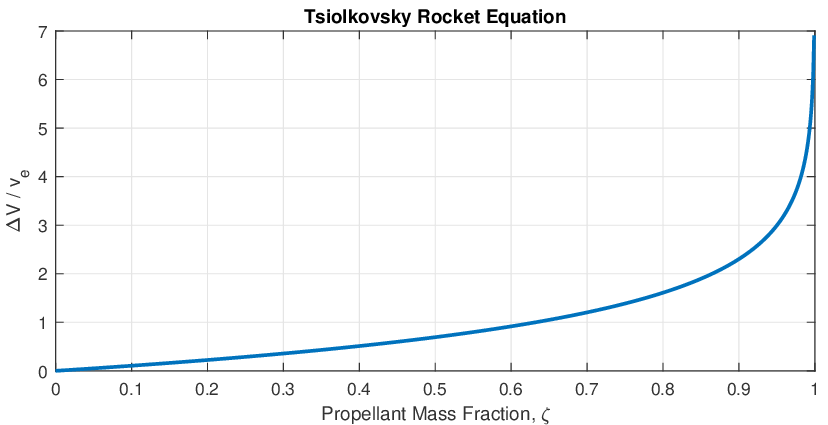
\includegraphics[width=0.7\textwidth]{Images/tsiolkovsky_graph.png}
    \caption{Rappresentazione grafica della "tirannia dell'equazione del razzo": la massa iniziale necessaria cresce in modo esponenziale all'aumentare della variazione di velocità richiesta ($\Delta v$).}
    \label{fig:tsiolkovsky_graph}
\end{figure}

%%%%%%%%%%%%%%%%%%%%%%%%%%%%%%%%%%%%%%%%%%%%%%%%%%%%%%%%%%%%%%%%%%%%%%%%%%%%%%%%%%%%%%%%%%%%%%%%%%%%%

\subsection{Il vincolo termodinamico insuperabile}
Di fronte alla crescita esponenziale della massa, l'unica soluzione matematica per ridurre il carico di propellente è aumentare l'impulso specifico $I_{sp}$, o la velocità di scarico $v_e$. Tuttavia, nei motori chimici questo parametro non può essere aumentato arbitrariamente. 

La velocità di espulsione dei gas è strettamente vincolata dal calore massimo che la reazione chimica riesce a sprigionare e dalla leggerezza dei prodotti che generano la spinta. Pur ricorrendo alla miscela propulsiva più efficiente a disposizione dell'ingegneria aerospaziale (idrogeno e ossigeno allo stato liquido, LOX/LH2), il limite termodinamico teorico dell'impulso specifico si scontra con una soglia invalicabile di circa 450-460 secondi. Semplicemente, nessuna reazione chimica conosciuta possiede un'intensità energetica sufficiente per superare questa barriera naturale.

Con dei limiti prestazionali così severi, l'esplorazione umana nello spazio profondo incontra una barriera fisica invalicabile \cite{mcconnell2023solarcruiser}. È in questo panorama di difficoltà termodinamiche che si inserisce la necessità di sviluppare propulsori di natura non-chimica. 
Se un veicolo potesse attingere la propria quantità di moto dall'esterno, eliminando del tutto la massa di propellente ($m_0 \approx m_f$), l'equazione di Tsiolkovsky decadrebbe, offrendo un impulso specifico potenzialmente infinito. Questa è l'esatta premessa teorica su cui si fonda la propulsione a vela solare.

%%%%%%%%%%%%%%%%%%%%%%%%%%%%%%%%%%%%%%%%%%%%%%%%%%%%%%%%%%%%%%%%%%%%%%%%%%%%%%%%%%%%%%%%%%%%%%%%%%%%%
%%%%%%%%%%%%%%%%%%%%%%%%%%%%%%%%%%%%%%%%%%%%%%%%%%%%%%%%%%%%%%%%%%%%%%%%%%%%%%%%%%%%%%%%%%%%%%%%%%%%%

\section{Fisica della radiazione elettromagnetica e pressione solare}
L'esplorazione sostenibile dello spazio profondo, quindi, richiede un cambio di strategia propulsiva che svincoli il veicolo dall'equazione di Tsiolkovsky. La propulsione a vela solare risponde a questa esigenza attingendo a una fonte di energia esterna e inesauribile: il Sole. Tuttavia, per comprendere matematicamente in che modo un raggio di luce possa generare una spinta meccanica tangibile su un oggetto macroscopico, è necessario esplorare la natura quantistica della radiazione elettromagnetica e definire le grandezze fisiche che governano l'ambiente interplanetario.

%%%%%%%%%%%%%%%%%%%%%%%%%%%%%%%%%%%%%%%%%%%%%%%%%%%%%%%%%%%%%%%%%%%%%%%%%%%%%%%%%%%%%%%%%%%%%%%%%%%%%

\subsection{Il dualismo onda-particella e la quantità di moto del fotone}
Dal punto di vista della fisica classica, la luce è descritta dalle equazioni dell'elettromagnetismo formulate da James Clerk Maxwell nel 1873. Secondo questo modello, la radiazione solare è un'onda elettromagnetica che si propaga nello spazio e che, incidendo su una superficie, esercita una pressione derivante dalla forza di Lorentz applicata alle cariche elettriche del materiale investito.

Sebbene il modello ondulatorio confermi l'esistenza della pressione di radiazione, la sua classificazione moderna si appoggia in modo più completo alla meccanica quantistica, in particolar modo riguardo alla propulsione. Nel 1905, Albert Einstein, spiegando l'effetto fotoelettrico, teorizzò che la luce non fosse unicamente un'onda continua, ma fosse quantizzata in pacchetti di energia, successivamente chiamati "fotoni".

Questa scoperta diede origine al concetto di \textit{dualismo onda-particella}, successivamente formalizzato e analizzato da Louis de Broglie. Un fotone è una particella elementare priva di massa ($m_0 = 0$). Tuttavia, secondo l'equazione dell'energia relativistica di Einstein:

\begin{equation}
    E^2 = (pc)^2 + (m_0 c^2)^2
\end{equation}

\begin{itemize}
    \item $E$ è l'energia totale della particella
    \item $p$ è la quantità di moto
    \item $c$ è la velocità della luce nel vuoto ($299\,792\,458 \, \text{m/s}$)
\end{itemize}

Ponendo la massa a riposo $m_0$ pari a zero, l'equazione si riduce a un'uguaglianza fondamentale per l'astrodinamica delle vele solari:

\begin{equation} \label{eq:quantita_moto_fotone}
    E = p \cdot c \implies p = \frac{E}{c}
\end{equation}

Questa relazione quantistica elementare è il cuore della propulsione fotonica \cite{mcinnes1999solar}. Essa dimostra che ogni singolo fotone che colpisce la membrana di una vela solare trasporta una quantità di moto infinitesimale. Quando il fotone viene assorbito o riflesso dalla superficie, la sua quantità di moto subisce una variazione ($\Delta p$). Per il principio di conservazione della quantità di moto, questa variazione deve essere trasferita alla vela sotto forma di impulso meccanico, generando una forza continua nel tempo.

%%%%%%%%%%%%%%%%%%%%%%%%%%%%%%%%%%%%%%%%%%%%%%%%%%%%%%%%%%%%%%%%%%%%%%%%%%%%%%%%%%%%%%%%%%%%%%%%%%%%%

\subsection{Costante solare e pressione in orbita terrestre}
Un singolo fotone possiede un'energia estremamente piccola. Affinché il trasferimento di quantità di moto diventi sufficiente per muovere un veicolo spaziale di svariati chilogrammi, è necessario calcolare l'effetto del flusso luminoso emesso da una stella.

Il Sole irradia energia in tutte le direzioni e la quantità di energia solare che attraversa perpendicolarmente una superficie unitaria in un secondo è definita come \textit{irradianza}. Alla distanza media tra la Terra e il Sole, definita come Unità Astronomica ($1 \, \text{AU} \approx 149.6 \times 10^6 \, \text{km}$), questo flusso prende il nome di \textbf{Costante Solare} ($W_E$). 

I dati moderni stabiliscono che il valore medio della costante solare all'esterno dell'atmosfera terrestre è:

\begin{equation}
    W_E \approx 1361 \, \text{W/m}^2 \quad \left( \text{oppure } \frac{\text{J}}{\text{s} \cdot \text{m}^2} \right)
\end{equation}

Sfruttando la relazione di Einstein ricavata in precedenza (Equazione \ref{eq:quantita_moto_fotone}), è possibile convertire questo flusso di energia in una pressione meccanica. Dividendo l'irradianza per la velocità della luce, si ottiene la pressione nominale della radiazione solare ($P_E$) misurata a un'Unità Astronomica di distanza su una superficie teorica perfettamente assorbente:

\begin{equation} \label{eq:pressione_terrestre}
    P_E = \frac{W_E}{c} = \frac{1361}{299\,792\,458} \approx 4.56 \times 10^{-6} \, \text{N/m}^2
\end{equation}

Questo valore estremamente piccolo (pari a circa 4.56 micronewton per metro quadrato) evidenzia il primo problema della propulsione a vela solare: la forza generata da un singolo metro quadrato di membrana è infinitesimale. Per ottenere una spinta significativa, è necessario dispiegare vele di dimensioni enormi (centinaia o migliaia di metri quadrati) e operare in un ambiente privo di attriti aerodinamici, come lo spazio interplanetario \cite{rodrigues2023review}.

%%%%%%%%%%%%%%%%%%%%%%%%%%%%%%%%%%%%%%%%%%%%%%%%%%%%%%%%%%%%%%%%%%%%%%%%%%%%%%%%%%%%%%%%%%%%%%%%%%%%%

\subsection{Decadimento spaziale e legge dell'inverso del quadrato}
La costante $P_E$ calcolata è valida esclusivamente nelle vicinanze dell'orbita terrestre (orbite LEO, MEO, GEO). Tuttavia, un simulatore astrodinamico progettato per missioni interplanetarie deve modellare dinamicamente la variazione della spinta in funzione della posizione del veicolo nel sistema solare.

L'energia emessa dal Sole si propaga radialmente e, poiché l'area di una sfera cresce proporzionalmente al quadrato del suo raggio ($A = 4\pi r^2$), la densità dei fotoni (e di conseguenza la pressione di radiazione) subisce una diminuzione quadratica.

Definendo $r_E$ come la distanza di riferimento (1 AU) e $r$ come l'effettiva distanza tra il Sole e la vela solare nell'istante di tempo considerato, l'intensità della pressione locale $P(r)$ è governata dalla legge dell'inverso del quadrato:

\begin{figure}[htbp!]
    \centering
    \includegraphics[width=0.75\textwidth]{Images/inverse_square_law.jpg}
    \caption{Propagazione sferica della radiazione elettromagnetica: la densità dei fotoni e la relativa pressione diminuiscono con il quadrato della distanza dalla sorgente solare.}
    \label{fig:inverse_square_law}
\end{figure}

\begin{equation} \label{eq:pressione_locale}
    P(r) = P_E \left( \frac{r_E}{r} \right)^2
\end{equation}

Questa equazione impone un vincolo molto preciso, che grazie al simulatore software sarà possibile verificare in tempo reale: la spinta di una vela solare non è costante, ma decresce rapidamente man mano che il veicolo si allontana dal Sole.
Avvicinandosi al Sole (ad esempio verso Venere o Mercurio, come avvenuto per la sonda IKAROS), il denominatore $r$ diminuisce, causando un incremento quadratico della spinta propulsiva e del carico termico. Al contrario, dirigendosi verso i pianeti esterni (Giove, Saturno), la pressione solare crolla drasticamente \cite{johnson2012status}. Ad esempio, a 5 AU (l'orbita di Giove), la spinta fotonica si riduce a solo 1/25 del valore misurato sulla Terra, rendendo le manovre a vela solare estremamente lente e complesse nello spazio profondo \cite{rodrigues2023review}.

%%%%%%%%%%%%%%%%%%%%%%%%%%%%%%%%%%%%%%%%%%%%%%%%%%%%%%%%%%%%%%%%%%%%%%%%%%%%%%%%%%%%%%%%%%%%%%%%%%%%%

\subsection{Luminosità solare}
Sebbene l'utilizzo della Costante Solare ($P_E$) sia comune per le missioni riferite unicamente all'orbita terrestre, lo sviluppo di un simulatore astrodinamico complesso richiede un approccio più generalizzato. 
Ecco perché un approccio più universale consiste nel calcolare la pressione di radiazione a partire dalla potenza totale emessa dal Sole, ovvero la sua luminosità ($L$), e adattare dinamicamente il calcolo in base alla posizione del veicolo.

Difatti il Sole si comporta come un'enorme lampada sferica che irradia energia in tutte le direzioni. La potenza totale emessa dal Sole è una costante fisica, espressa in $W$ che può essere calcolata a partire dalla Costante Solare e dall'area della sfera di raggio 1 AU:

\begin{equation}
    L \approx 3.828 \times 10^{26} \, \text{W}
\end{equation}

Poiché questa immensa energia si propaga nello spazio vuoto distribuendosi sulla superficie di una sfera in continua espansione (la cui area è $4\pi r^2$), il flusso energetico locale a una qualsiasi distanza $r$ dal centro del Sole è dato da:

\begin{equation}
    W(r) = \frac{L}{4 \pi r^2} \quad \left[ \frac{\text{W}}{\text{m}^2} \right]
\end{equation}

\begin{figure}[htbp!]
    \centering
    % 
\includegraphics[width=0.8\textwidth]{Images/inverse_square_luminosity.jpg}
    \caption{Rappresentazione geometrica della Legge dell'Inverso del Quadrato: la Potenza totale emessa dalla stella (Luminosità L) si diluisce sulla superficie di sfere concentriche in espansione, riducendo l'intensità del flusso locale in proporzione a $1/r^2$.}
    \label{fig:luminosity_inverse_square}
\end{figure}

Dividendo questo flusso per la velocità della luce $c$, si ottiene l'equazione universale della pressione fotonica locale con cui è possibile calcolare la forza istantanea che agisce su una vela solare in qualsiasi punto del sistema solare:

\begin{equation} \label{eq:pressione_luminosita}
    P(r) = \frac{L}{4 \pi r^2 c}
\end{equation}

Questa formulazione è più flessibile e adatta a un simulatore astrodinamico, poiché consente di modellare con precisione la spinta fotonica in qualsiasi punto del sistema solare, tenendo conto della posizione dinamica del veicolo rispetto al Sole. È proprio questa equazione che è stata implementata nel simulatore sviluppato in Unreal Engine, permettendo il calcolo istantaneo della pressione di radiazione locale e dell'accelerazione risultante durante l'intero arco della missione.

%%%%%%%%%%%%%%%%%%%%%%%%%%%%%%%%%%%%%%%%%%%%%%%%%%%%%%%%%%%%%%%%%%%%%%%%%%%%%%%%%%%%%%%%%%%%%%%%%%%%%
%%%%%%%%%%%%%%%%%%%%%%%%%%%%%%%%%%%%%%%%%%%%%%%%%%%%%%%%%%%%%%%%%%%%%%%%%%%%%%%%%%%%%%%%%%%%%%%%%%%%%

\section{Modellazione ottica vettoriale e interazione fotonica}
Avendo definito la pressione di radiazione solare locale $P(r)$, è possibile calcolare la forza totale che agisce su una vela solare. Tuttavia, questa forza non è semplicemente il prodotto scalare tra $P(r)$ e l'area geometrica della vela. La spinta risultante dipende da una complessa interazione tra i fotoni incidenti e la superficie della membrana, che coinvolge fenomeni di riflessione, assorbimento e diffusione.

%%%%%%%%%%%%%%%%%%%%%%%%%%%%%%%%%%%%%%%%%%%%%%%%%%%%%%%%%%%%%%%%%%%%%%%%%%%%%%%%%%%%%%%%%%%%%%%%%%%%%

\subsection{Area effettiva e angolo di incidenza}
Il primo parametro fondamentale per calcolare l'interazione fotonica è la determinazione della parte della vela effettivamente esposta al flusso di fotoni. La forza generata dalla pressione solare non dipende dall'area totale della vela, ma dall'area proiettata perpendicolarmente alla direzione dei raggi solari.

Per prima cosa è necessario definire un sistema di riferimento solidale alla vela solare in cui $\mathbf{n}$ rappresenta il versore normale (perpendicolare) alla superficie della vela. Inoltre, è utile dichiarare $\mathbf{u}$ come il versore direzione dell'illuminazione, ovvero il vettore che punta dal centro di massa del veicolo verso il Sole. 

L'angolo compreso tra il versore normale $\mathbf{n}$ e la direzione dei raggi solari $\mathbf{u}$ prende il nome di \textit{angolo di incidenza} ($\alpha$). 
La superficie della vela non sempre è completamente esposta al flusso solare. L'area effettiva che riceve i fotoni dipende dall'orientamento della vela rispetto al Sole ed è calcolata così:

\begin{equation}
    A_{\text{eff}} = A \cos(\alpha)
\end{equation}

\begin{figure}[htbp!]
    \centering
    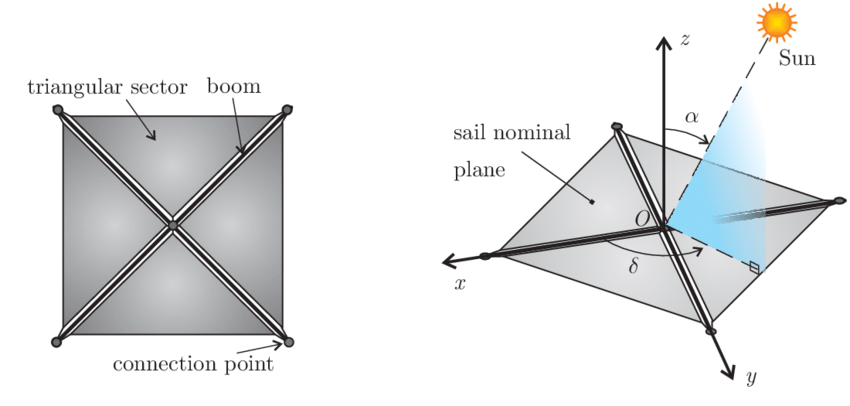
\includegraphics[width=0.6\textwidth]{Images/sail_geometry.png}
    \caption{Schema vettoriale dell'interazione fotonica: il versore normale $\mathbf{n}$, la direzione dei raggi solari $\mathbf{u}$ e l'angolo di incidenza $\alpha$ che determina l'area effettivamente esposta.}
    \label{fig:sail_geometry}
\end{figure}

Questa relazione geometrica implica che la vela cattura il massimo della quantità di moto quando è orientata frontalmente al Sole ($\alpha = 0^\circ$, dove $\cos(0) = 1$). Man mano che la vela viene inclinata, l'area esposta diminuisce, fino ad annullarsi completamente quando la vela è posta "di taglio" rispetto ai raggi solari ($\alpha = 90^\circ$, dove $\cos(90) = 0$).

%%%%%%%%%%%%%%%%%%%%%%%%%%%%%%%%%%%%%%%%%%%%%%%%%%%%%%%%%%%%%%%%%%%%%%%%%%%%%%%%%%%%%%%%%%%%%%%%%%%%%

\subsection{Fenomeni di ombreggiamento e auto-occlusione}
Il modello matematico finora descritto assume che la vela solare sia una superficie piana e perfettamente esposta ai raggi solari. Nella realtà operativa, tuttavia, la sonda è una struttura tridimensionale complessa. Elementi come il modulo centrale (\textit{bus}), i bracci telescopici per il dispiegamento (\textit{booms}) e la strumentazione di bordo sono posti tra il Sole e la vela riflettente, proiettando delle ombre.

Questo fenomeno, noto come \textbf{auto-occlusione}, azzera la spinta fotonica nelle zone oscurate. Le conseguenze sulla dinamica del veicolo sono due: 
\begin{itemize}
    \item Una riduzione netta della spinta propulsiva totale.
    \item Uno spostamento asimmetrico del centro di pressione; questo può generare un momento torcente che induce rotazioni non pianificate del veicolo, complicando le manovre di controllo d'assetto.
\end{itemize}

Oltre a ciò, la vela può presentare deformazioni strutturali, pieghe o irregolarità che causano ulteriori ombre.

Per calcolare con precisione l'area effettivamente illuminata, l'equazione algebrica $A_{\text{eff}} = A \cos(\alpha)$ non basta.
Il calcolo deve essere impostato come un integrale di superficie che includa una funzione di visibilità $v(x,y)$, la quale restituisce il valore $1$ se il punto è direttamente illuminato e il valore $0$ se è in ombra:

\begin{equation}
    A_{\text{eff}} = \int_{A} v(x,y) \cos(\alpha) \, dA
\end{equation}

\begin{figure}[htbp!]
    \centering
    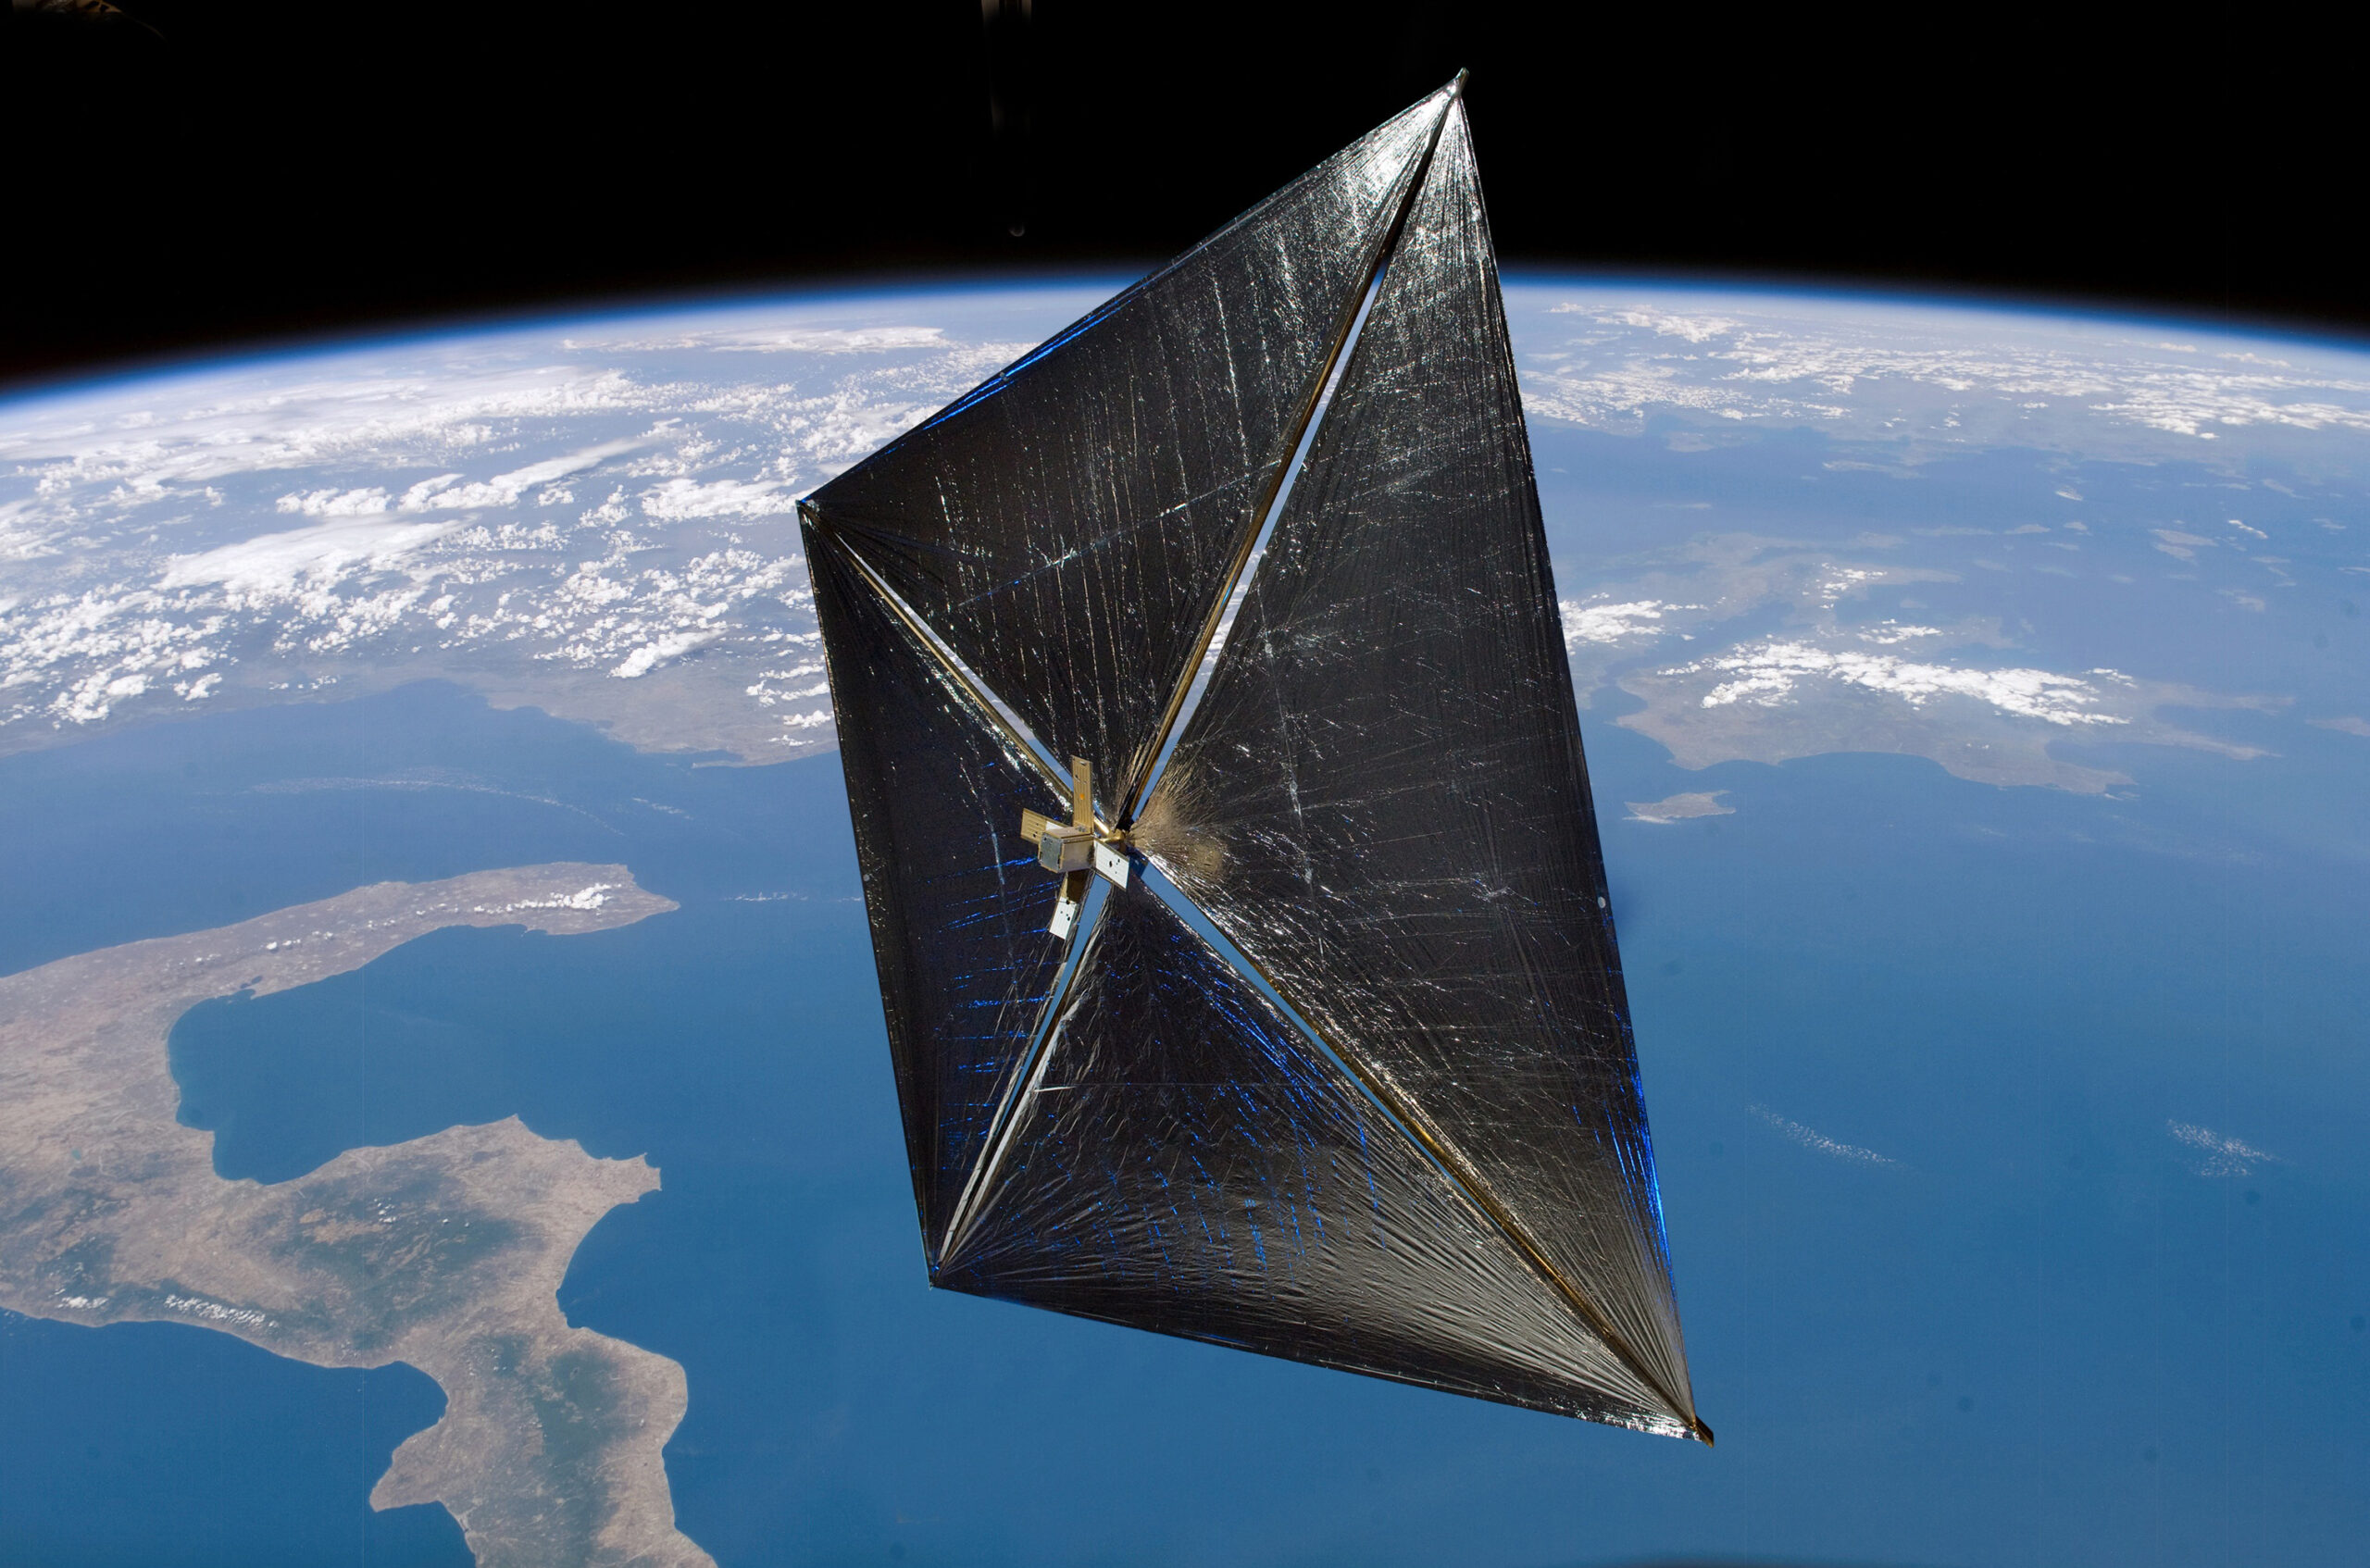
\includegraphics[width=0.7\textwidth]{Images/sail_shadowing.jpg}
    \caption{Rappresentazione concettuale dell'auto-occlusione: i componenti strutturali del veicolo proiettano ombre sulla membrana riflessiva, rendendo necessario il calcolo locale dell'area effettivamente illuminata.}
    \label{fig:sail_shadowing}
\end{figure}

Purtroppo questo calcolo risulta essere impossibile da risolvere analiticamente, poiché la funzione di visibilità $v(x,y)$ dipende dalla geometria complessa del veicolo e dalla posizione relativa del Sole.
Questo ostacolo giustifica la necessità di utilizzare un motore grafico: algoritmi di calcolo spaziale discretizzato, come il \textit{Ray Casting}, permettono di campionare dinamicamente la funzione di visibilità $v(x,y)$ sulla geometria della vela, risolvendo il problema delle ombre in tempo reale.

%%%%%%%%%%%%%%%%%%%%%%%%%%%%%%%%%%%%%%%%%%%%%%%%%%%%%%%%%%%%%%%%%%%%%%%%%%%%%%%%%%%%%%%%%%%%%%%%%%%%%

\subsection{Occlusione ambientale e asimmetria di spinta}
Oltre all'auto-occlusione causata dai componenti specifici della vela solare, un simulatore astrodinamico ad alta fedeltà deve modellare accuratamente l'\textbf{occlusione ambientale}. Questo fenomeno si verifica quando un corpo celeste (ad esempio un pianeta, una luna o un asteroide) si interpone tra il Sole e la vela, causando un'occlusione totale o parziale.

Se un'eclissi totale comporta semplicemente l'azzeramento globale della spinta fotonica, le fasi di transizione o di occlusione parziale introducono problemi molto più complessi. Quando un corpo oscura solo una porzione della vela solare, si instaura una forte asimmetria nella distribuzione delle forze. 

Dal punto di vista della meccanica dei corpi rigidi, la differenza di pressione causata dalla radiazione solare, tra la zona in ombra e la superficie illuminata, dà luogo ad una discordanza tra i due centri di pressione fotonica e di massa del veicolo, generando un momento torcente che provoca la rotazione del veicolo.

Il simulatore sviluppato in questo elaborato è capace di analizzare questa complessa casistica.
In particolar modo, grazie alla modellazione tridimensionale della vela solare e alla simulazione dinamica del sistema solare, è possibile calcolare in tempo reale l'effetto di un'eclissi parziale, prevedendo con precisione la forza risultante e il momento torcente che agisce sul veicolo durante le fasi di transizione.


\begin{figure}[htbp!]
    \centering
    % 
\includegraphics[width=0.7\textwidth]{Images/partial_eclipse_torque.jpg}
    \caption{Effetto dell'occlusione ambientale parziale: l'asimmetria di illuminazione sposta il centro di pressione rispetto al centro di massa, generando un momento torcente (\textit{torque}) che induce il rotolamento del veicolo.}
    \label{fig:eclipse_torque}
\end{figure}

L'effetto di questo momento torcente è di fondamentale importanza per la dinamica del veicolo, poiché può indurre un "rotolamento" incontrollato che a sua volta può compromettere l'orientamento dei pannelli solari e interrompere i collegamenti telemetrici con la Terra. Inoltre costringe il sistema di controllo d'assetto a consumare preziose risorse propulsive per contrastare queste rotazioni, riducendo ulteriormente l'efficienza complessiva della missione \cite{rodrigues2023review}.

%%%%%%%%%%%%%%%%%%%%%%%%%%%%%%%%%%%%%%%%%%%%%%%%%%%%%%%%%%%%%%%%%%%%%%%%%%%%%%%%%%%%%%%%%%%%%%%%%%%%%

\subsection{Il modello ottico ideale (Riflessione speculare perfetta)}
Per comprendere l'origine delle componenti di forza, è utile partire da un modello ideale in cui la superficie della vela solare è perfettamente liscia e riflettente, senza alcuna perdita di energia.
In questo scenario ideale, si assume che il 100\% dei fotoni incidenti venga riflesso in modo perfettamente elastico (riflessione speculare), senza alcuna perdita di energia per assorbimento o diffusione. 

Quando un fotone con quantità di moto $p$ colpisce la superficie con un angolo $\alpha$, esso viene riflesso con il medesimo angolo rispetto alla normale. La variazione della quantità di moto del fotone lungo l'asse tangenziale alla vela è nulla, mentre lungo l'asse normale alla vela è pari a $2p \cos(\alpha)$. 

Integrando questo scambio di quantità di moto sull'intera area esposta $A \cos(\alpha)$ e moltiplicandolo per il flusso di fotoni, si ottiene la forza della Pressione di Radiazione Solare nel caso ideale ($\mathbf{F}_{\text{ideale}}$). Poiché in un urto elastico la componente trasversale si annulla, l'intero vettore forza è diretto lungo la normale $\mathbf{n}$ della vela:

\begin{equation} \label{eq:srp_ideale}
    \mathbf{F}_{\text{ideale}} = 2 P(r) A \cos^2(\alpha) \mathbf{n}
\end{equation}
Per comprendere l'origine del termine $\cos^2(\alpha)$, è necessario analizzare in dettaglio l'interazione fotonica per ogni singolo fotone incidente.
Considerando un fotone incidente che trasporta quantità di moto $p = E/c$. 

Quando il fotone colpisce la superficie della vela con angolo di incidenza $\alpha$ (misurato rispetto alla normale $\mathbf{n}$), la sua quantità di moto può essere ripartita in due componenti perpendicolari tra loro:
\begin{itemize}
    \item Componente normale: $p_n = p \cos(\alpha)$
    \item Componente tangenziale: $p_t = p \sin(\alpha)$
\end{itemize}

Nel caso di riflessione speculare perfetta, il fotone rimbalza elasticamente mantenendo l'angolo di incidenza. La componente tangenziale rimane invariata ($p_t' = p_t$), mentre la componente normale si inverte ($p_n' = -p_n$). La variazione totale di quantità di moto del fotone lungo la direzione normale è:

\begin{equation}
    \Delta p_n = p_n' - p_n = -p\cos(\alpha) - p\cos(\alpha) = -2p\cos(\alpha)
\end{equation}

Per il principio di conservazione della quantità di moto, la vela riceve un impulso diretto lungo la propria normale pari a:

\begin{equation}
    \Delta p_{\text{vela}} = 2p\cos(\alpha) = 2\frac{E}{c}\cos(\alpha)
\end{equation}

Tuttavia, il flusso luminoso non interagisce con l'intera area geometrica $A$ della membrana, bensì soltanto con la porzione effettivamente esposta alla radiazione, la quale si riduce all'aumentare dell'inclinazione del veicolo:

\begin{equation}
    A_{\text{eff}} = A\cos(\alpha)
\end{equation}

La forza totale esercitata sulla vela si ricava integrando la pressione locale $P(r)$ sull'area effettiva, tenendo conto del fattore di riflessione elastica lungo la normale. Moltiplicando questi termini si ottiene:

\begin{equation}
    F = P(r) \cdot A_{\text{eff}} \cdot (2\cos\alpha) = 2P(r)A\cos^2(\alpha)
\end{equation}

Il termine quadratico $\cos^2(\alpha)$ è di fondamentale importanza nell'astrodinamica fotonica e ha una duplice origine fisica: un primo fattore $\cos(\alpha)$ deriva dalla riduzione puramente geometrica dell'area intercettata ($A_{\text{eff}}$), mentre il secondo $\cos(\alpha)$ deriva dalla proiezione dell'impulso trasferito lungo l'asse normale alla superficie.

Questa dipendenza quadratica dimostra che la spinta di una vela solare diminuisce molto rapidamente rispetto alla semplice inclinazione della vela: a $30^\circ$ di incidenza, la forza propulsiva si riduce al $75\%$ del suo valore ($\cos^2(30^\circ) \approx 0.75$), a $45^\circ$ di inclinazione invece la forza scende al $50\%$ \cite{mcinnes1999solar}.

%%%%%%%%%%%%%%%%%%%%%%%%%%%%%%%%%%%%%%%%%%%%%%%%%%%%%%%%%%%%%%%%%%%%%%%%%%%%%%%%%%%%%%%%%%%%%%%%%%%%%

\subsection{Il modello ottico realistico (Superfici non ideali)}
Il modello ideale descritto dall'Equazione \ref{eq:srp_ideale} è un'ottima approssimazione per i calcoli preliminari, ma risulta inadeguato per un simulatore informatico \textit{High-Fidelity}. Nella realtà, nessun materiale polimerico metallizzato (come il Kapton alluminato) possiede una riflettività del 100\%. 

L'interazione della luce con un materiale reale è un fenomeno complesso in cui i fotoni incidenti subiscono rimbalzi differenti. Per modellare matematicamente questo comportamento, la letteratura aerospaziale definisce tre coefficienti ottici, la cui somma conserva l'energia totale (deve essere pari a 1):

\begin{equation}
    \rho_s + \rho_d + \alpha_a = 1
\end{equation}

Questi parametri descrivono le tre reazioni ottiche della superficie:
\begin{itemize}
    \item \textbf{Riflessione speculare ($\rho_s$):} La parte di fotoni che rimbalza elasticamente mantenendo l'angolo di incidenza. Genera una forza diretta unicamente lungo la normale $\mathbf{n}$.
    \item \textbf{Riflessione diffusa ($\rho_d$):} La parte di fotoni che, a causa delle irregolarità del materiale, viene riflessa in direzioni casuali. Questa componente introduce una forza di taglio parallela alla superficie della vela, deviando la forza totale rispetto alla normale $\mathbf{n}$.
    \item \textbf{Assorbimento ($\alpha_a$):} La frazione di fotoni che non viene riflessa, ma assorbita dal materiale. Questa componente non genera "rimbalzo", trasferendo la propria quantità di moto esclusivamente nella direzione di incidenza originale dei raggi solari ($\mathbf{u}$). L'energia assorbita si trasforma poi in calore termico.
\end{itemize}

\begin{figure}[htbp!]
    \centering
    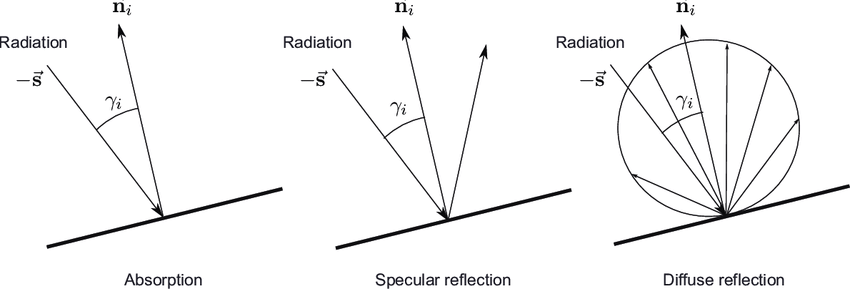
\includegraphics[width=0.8\textwidth]{Images/optical_reflection_model.png}
    \caption{Confronto visivo tra i fenomeni ottici su una superficie non ideale: riflessione speculare ($\rho_s$), riflessione diffusa ($\rho_d$) e assorbimento ($\alpha_a$).}
    \label{fig:optical_model}
\end{figure}

La coesistenza di questi tre fenomeni fa sì che la forza risultante su una vela reale non sia mai perfettamente allineata al versore normale $\mathbf{n}$ (tranne quando $\alpha = 0^\circ$). L'assorbimento e la diffusione introducono un'asimmetria che genera una forza di taglio (\textit{shear force}) parallela alla superficie della vela, un elemento critico che può deviare la traiettoria orbitale.

%%%%%%%%%%%%%%%%%%%%%%%%%%%%%%%%%%%%%%%%%%%%%%%%%%%%%%%%%%%%%%%%%%%%%%%%%%%%%%%%%%%%%%%%%%%%%%%%%%%%%

\subsection{L'equazione vettoriale dell'accelerazione SRP}
Volendo quindi determinare l'effettiva spinta generata sul veicolo, i valori derivanti dai diversi fenomeni ottici descritti devono essere raggruppati in un'unica formula. Per la buona riuscita di questa operazione, si introduce il versore trasversale $\mathbf{t}$, definito come parallelo al piano della vela solare e complanare al piano formato dalla normale $\mathbf{n}$ e dalla direzione di incidenza dei raggi solari $\mathbf{u}$.

L'accelerazione totale generata dalla Pressione di Radiazione Solare ($\mathbf{a}_{\text{SRP}}$) su un veicolo di massa $m$ e area $A$, inclinato di un angolo $\alpha$ lungo la direzione del versore $\mathbf{t}$, è espressa dalla seguente equazione vettoriale \cite{simo2016realistic}:

\begin{equation} \label{eq:srp_force_vector}
    \mathbf{a}_{\text{SRP}} = \frac{P(r) A}{m} \cos(\alpha) \left[ \left(1 + \rho_s \cos(2\alpha) + \frac{2}{3}\rho_d \cos(\alpha) \right)\mathbf{n} + \left(\rho_s \sin(2\alpha) + \rho_d \sin(\alpha) \right)\mathbf{t} \right]
\end{equation}

Questa formulazione mostra l'intera fisica propulsiva del modello non-ideale. Al suo interno è possibile distinguere chiaramente due valori ortogonali: 
\begin{itemize}
    \item La componente associata al versore $\mathbf{n}$ rappresenta la \textbf{spinta normale}, ovvero l'accelerazione generata lungo la direzione normale alla superficie della vela.
    \item La componente associata al versore $\mathbf{t}$ rappresenta la \textbf{forza di taglio} (\textit{shear force}), elemento critico per la navigazione solare poiché in grado di generare spostamenti laterali della traiettoria orbitale.
\end{itemize}

Calcolare questa espressione vettoriale istante per istante, ricavando ogni volta le normali geometriche $\mathbf{n}$ e osservando come i raggi incidono sulla vela, rappresenta la prima sfida che il simulatore software in C++, sviluppata in Unreal Engine e presentata nel capitolo successivo, deve svolgere.

%%%%%%%%%%%%%%%%%%%%%%%%%%%%%%%%%%%%%%%%%%%%%%%%%%%%%%%%%%%%%%%%%%%%%%%%%%%%%%%%%%%%%%%%%%%%%%%%%%%%%
%%%%%%%%%%%%%%%%%%%%%%%%%%%%%%%%%%%%%%%%%%%%%%%%%%%%%%%%%%%%%%%%%%%%%%%%%%%%%%%%%%%%%%%%%%%%%%%%%%%%%

\section{Parametri di design e sintesi della dinamica orbitale}
Attraverso le equazioni esposte nei paragrafi precedenti, è possibile calcolare con precisione la forza di pressione solare che agisce su una vela in qualsiasi punto del sistema solare, tenendo conto dell'orientamento della vela e delle proprietà ottiche del materiale.
Tuttavia, il reale comportamento cinematico del veicolo spaziale sottoposto alla perturbazione solare non dipende esclusivamente dall'efficienza ottica del materiale o dalla distanza dal Sole, ma è rigidamente vincolata dalla geometria strutturale e dalla distribuzione delle masse del veicolo. Ecco perché diventa utile definire alcuni parametri di design che sintetizzano le caratteristiche macroscopiche del veicolo e che permettono di valutare le prestazioni propulsive in modo più immediato, indipendentemente dall'orbita specifica o dalle condizioni operative.

%%%%%%%%%%%%%%%%%%%%%%%%%%%%%%%%%%%%%%%%%%%%%%%%%%%%%%%%%%%%%%%%%%%%%%%%%%%%%%%%%%%%%%%%%%%%%%%%%%%%%

\subsection{Il Carico Alare (Sail Loading)}
Il parametro di design più critico nella progettazione di un veicolo a propulsione fotonica è il Carico Alare (\textit{Sail Loading}), solitamente indicato con la lettera greca $\sigma$. Questo è definito come il rapporto tra la massa totale del veicolo spaziale e l'area totale della membrana dispiegata per la "cattura" dei fotoni:

\begin{equation} \label{eq:sail_loading}
    \sigma = \frac{m}{A} \quad \left[ \frac{\text{kg}}{\text{m}^2} \right]
\end{equation}

La massa $m$ al numeratore comprende tutti i componenti del veicolo: la massa del carico utile (\textit{payload} scientifico), la massa riguardante i sistemi satellitari (sistemi di comunicazione, computer di bordo, pannelli solari, giroscopi per la rotazione della vela), la massa dei bracci telescopici di dispiegamento (\textit{booms}) e, infine, la massa della membrana stessa.

L'obiettivo primario durante il dimensionamento di una missione è minimizzare $\sigma$. Un valore di \textit{Sail Loading} basso indica infatti che il veicolo è molto leggero rispetto alla superficie che espone alla radiazione solare, massimizzando così l'accelerazione generata dalla pressione di radiazione.
Le vele solari di prima generazione (come IKAROS) presentavano valori di $\sigma$ relativamente alti a causa dell'utilizzo di membrane più spesse e meccanismi di dispiegamento delle stesse più pesanti. Attraverso gli sviluppi moderni e futuri si può mirare a spingere questo valore al di sotto dei $10 \, \text{g/m}^2$, impiegando pellicole di spessore sub-micrometrico e strutture in fibra di carbonio, che sono in grado di resistere alle sollecitazioni meccaniche e termiche dello spazio profondo pur mantenendo una massa estremamente ridotta \cite{rodrigues2023review} \cite{johnson2012status}.

%%%%%%%%%%%%%%%%%%%%%%%%%%%%%%%%%%%%%%%%%%%%%%%%%%%%%%%%%%%%%%%%%%%%%%%%%%%%%%%%%%%%%%%%%%%%%%%%%%%%%

\subsection{Accelerazione Caratteristica}
Un altro parametro di design fondamentale è l'Accelerazione Caratteristica ($a_c$). Esso rappresenta il valore massimo di accelerazione che una vela solare può generare quando è esposta alla luce solare nelle condizioni più favorevoli: posizionata a 1 Unità Astronomica dal Sole e orientata perpendicolarmente rispetto ai raggi solari ($\alpha = 0^\circ$).

Sostituendo l'equazione del \textit{Sail Loading} ($\sigma$) all'interno del modello ottico realistico discusso in precedenza (Equazione \ref{eq:srp_force_vector}), e considerando che per $\alpha = 0^\circ$ la componente trasversale si annulla, si ricava la formula analitica dell'Accelerazione Caratteristica:

\begin{equation} \label{eq:accelerazione_caratteristica}
    a_c = \frac{P_E}{\sigma} \left( 1 + \rho_s + \frac{2}{3}\rho_d \right) \quad \left[ \frac{\text{m}}{\text{s}^2} \right]
\end{equation}

Questo valore rappresenta un fondamentale parametro di riferimento per la validazione dell'ambiente virtuale. Al fine di certificare l'accuratezza del simulatore, durante le fasi di collaudo i vettori tridimensionali restituiti in tempo reale da Unreal Engine dovranno essere confrontati con il valore $a_c$ teorico, a patto che la vela simulata venga esposta alle condizioni operative ideali.

%%%%%%%%%%%%%%%%%%%%%%%%%%%%%%%%%%%%%%%%%%%%%%%%%%%%%%%%%%%%%%%%%%%%%%%%%%%%%%%%%%%%%%%%%%%%%%%%%%%%%

\subsection{Numero di Leggerezza}
Un ulteriore parametro di design di grande interesse astrodinamico è il Numero di Leggerezza (\textit{Lightness Number}, $\beta$). Esso esprime il rapporto tra la massima accelerazione repulsiva della pressione solare $a_c$ e l'attrazione gravitazionale del Sole $g_{\text{sole}}$ alla stessa distanza:

\begin{equation}
    \beta = \frac{a_c}{g_{\text{sole}}}
\end{equation}

Il Numero di Leggerezza è un valore che mostra rapidamente la capacità propulsiva di una vela solare rispetto alla forza gravitazionale che agisce su di essa. Un valore di $\beta < 1$ indica che la forza gravitazionale del Sole vince su quella fotonica, di conseguenza la vela non potrà mai "sfuggire" dal sistema solare e per acquisire velocità dovrà rimanere in orbita per molto. Al contrario, un valore di $\beta > 1$ indica che la spinta fotonica supera la gravità solare, permettendo al veicolo di "sfuggire" direttamente dal sistema solare seguendo una traiettoria iperbolica, senza necessità di lunghi periodi di accelerazione orbitale \cite{mcinnes1999solar}.

%%%%%%%%%%%%%%%%%%%%%%%%%%%%%%%%%%%%%%%%%%%%%%%%%%%%%%%%%%%%%%%%%%%%%%%%%%%%%%%%%%%%%%%%%%%%%%%%%%%%%

\subsection{Il campo gravitazionale primario e la meccanica orbitale}
Seppur fino ad ora si sia parlato esclusivamente delle forze riguardanti la dinamica fotonica, è importante evidenziare che la vela solare è comunque sempre soggetta alla forza gravitazionale di uno o più corpi celesti.

Il veicolo fotonico è infatti governato dalle leggi della meccanica orbitale, ed in particolar modo dalla legge di gravitazione universale formulata da Isaac Newton.
Questa afferma che ogni corpo dotato di massa esercita un'attrazione gravitazionale su ogni altro corpo, con una forza $\mathbf{F}_g$ che è direttamente proporzionale al prodotto delle loro masse e inversamente proporzionale al quadrato della distanza che unisce i due centri di massa:

\begin{equation}
    \mathbf{F}_g = - G \frac{M \cdot m}{r^2} \mathbf{\hat{r}}
\end{equation}

dove:
\begin{itemize}
    \item $G$ è la Costante di Gravitazione Universale ($6.674 \times 10^{-11} \, \text{m}^3 \text{kg}^{-1} \text{s}^{-2}$), fondamentale che quantifica l'intensità gravitazionale;
    \item $M$ è la massa del corpo centrale, espressa in $\text{kg}$, che genera il campo gravitazionale;
    \item $m$ è la massa del veicolo spaziale, che subisce l'attrazione gravitazionale generata dal corpo centrale;
    \item $r$ è la distanza tra i centri di massa del corpo centrale e del veicolo spaziale, misurata in metri;
    \item $\mathbf{\hat{r}}$ è il versore che indica la direzione dal centro del pianeta verso il veicolo spaziale, con il segno negativo che indica che la forza è attrattiva (verso il corpo centrale).
\end{itemize}


Affinché il veicolo spaziale non venga attratto verso il corpo centrale, è necessario che la forza di gravità sia controbilanciata da una forza centrifuga generata dal moto orbitale del veicolo.
Questa velocità orbitale, che dipende dalla distanza $r$ e dalla massa del corpo centrale $M$, è quella necessaria per mantenere un'orbita stabile.

Tale velocità si ricava uguagliando la forza gravitazionale alla forza centrifuga ($m v^2 / r$) e risolvendo per $v$, ottenendo così la formula della velocità orbitale circolare:

\begin{equation}
    v = \sqrt{\frac{G \cdot M}{r}}
\end{equation}

La moltiplicazione tra $G$ e $M$ è un prodotto così ricorrente nella meccanica orbitale che viene spesso accorpato in un unico parametro, noto come \textit{parametro gravitazionale standard} ($\mu$) definito come:

\begin{equation}
    \mu = G \cdot M
\end{equation}

È dunque possibile esprimere anche la forza gravitazionale in termini di accelerazione, dividendo $\mathbf{F}_g$ per la massa del veicolo $m$:

\begin{equation}
    \mathbf{a}_g = \frac{\mathbf{F}_g}{m} = - G \frac{M}{r^2} \mathbf{\hat{r}} = - \frac{\mu}{r^2} \mathbf{\hat{r}}
\end{equation}
 
Inoltre, tenendo conto che il versore $\mathbf{\hat{r}}$ è definito come $\mathbf{r}/r$, dove $\mathbf{r}$ è il vettore posizione del veicolo spaziale rispetto al corpo centrale è possibile esprimere tale accelerazione in forma vettoriale.
Infine quindi, l'equazione vettoriale dell'accelerazione gravitazionale centrale che agisce su un veicolo spaziale in orbita attorno a un corpo centrale è:

\begin{equation}
    \mathbf{a}_g(\mathbf{r}) = - \frac{\mu}{r^3} \mathbf{r}
\end{equation}

\begin{figure}[htbp!]
    \centering
    % \includegraphics[width=0.6\textwidth]{Images/gravity_vector_diagram.jpg}
    \caption{Diagramma vettoriale dell'accelerazione gravitazionale centrale. Il vettore posizione $\mathbf{r}$ è diretto dal fuoco all'oggetto; il vettore accelerazione $\mathbf{a}_g$ è sempre diretto in verso opposto (verso il corpo attrattore), giustificando il segno negativo nell'equazione vettoriale.}
    \label{fig:gravity_vector}
\end{figure}

%%%%%%%%%%%%%%%%%%%%%%%%%%%%%%%%%%%%%%%%%%%%%%%%%%%%%%%%%%%%%%%%%%%%%%%%%%%%%%%%%%%%%%%%%%%%%%%%%%%%%

\subsection{Sintesi finale: l'Equazione del Moto}
Ora che sono state definite sia gravità ($\mathbf{a}_g$) che spinta fotonica ($\mathbf{a}_{\text{SRP}}$), è possibile unirle per ottenere l'equazione finale che descrive il movimento della vela solare.

Per mantenere il calcolo gestibile, si ricorre solitamente a un'approssimazione pratica: vengono ignorate le forze secondarie marginali, come l'attrito dell'alta atmosfera, l'attrazione della Luna o la forma non perfettamente sferica della Terra. Fatto ciò, l'accelerazione totale della navicella è semplicemente la somma di chi la tira verso il basso (il pianeta) e di chi la spinge via (il Sole):

\begin{equation} \label{eq:equazione_moto_finale}
    \ddot{\mathbf{r}} = \mathbf{a}_g(\mathbf{r}) + \mathbf{a}_{\text{SRP}}(\mathbf{r}, \alpha, \rho_s, \rho_d)
\end{equation}

Espandendo questa formula e inserendo tutte le equazioni che sono state dimostrate fino ad ora, compreso l'uso della Luminosità solare ($L$) per calcolare la pressione, è possibile ottenere l'equazione completa del sistema:

\begin{equation}
    \frac{d^2\mathbf{r}}{dt^2} = - \frac{\mu}{r^3} \mathbf{r} + \frac{L \cdot A}{4 \pi r^2 c \cdot m} \cos(\alpha) \left[ \left(1 + \rho_s \cos(2\alpha) + \frac{2}{3}\rho_d \cos(\alpha) \right)\mathbf{n} + \left(\rho_s \sin(2\alpha) + \rho_d \sin(\alpha) \right)\mathbf{t} \right]
\end{equation}

\begin{figure}[htbp!]
    \centering
    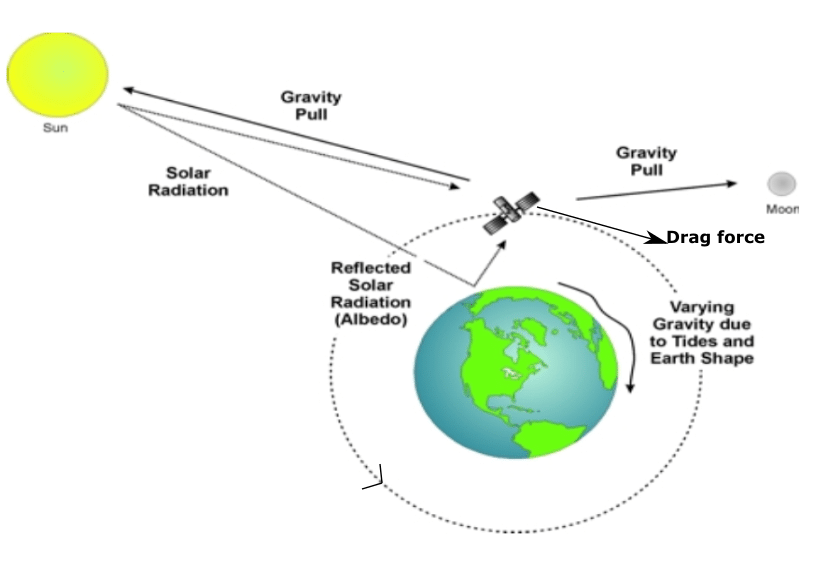
\includegraphics[width=0.7\textwidth]{Images/orbital_forces.png}
    \caption{Diagramma delle forze in gioco: l'accelerazione totale della vela solare è data dalla somma vettoriale tra la gravità ($\mathbf{a}_g$) e la perturbazione fotonica ($\mathbf{a}_{\text{SRP}}$).}
    \label{fig:orbital_forces}
\end{figure}

Come è facile intuire, questa equazione è estremamente complessa. Tale complessità rende notevolmente difficile la possibilità di prevedere con precisione la traiettoria del veicolo spaziale, poiché ogni variabile è in continua evoluzione durante il viaggio. Man mano che il veicolo viaggia, la distanza ($r$) varia, modificando contemporaneamente sia l'attrazione gravitazionale che l'intensità della luce. Inoltre, ogni minima rotazione della vela cambia gli angoli di incidenza e i vettori di direzione ($\mathbf{n}$ e $\mathbf{t}$).

A causa di queste continue variazioni, è matematicamente impossibile risolvere questa equazione "a mano" con carta e penna per prevedere dove si troverà la vela tra un mese. L'unico modo per tracciare la rotta è usare un approccio virtuale: far calcolare al computer questa enorme formula ogni istante. Il prossimo capitolo spiegherà proprio come la programmazione a oggetti e il motore grafico Unreal Engine 5 siano stati impiegati per compiere questo complesso lavoro.

%%%%%%%%%%%%%%%%%%%%%%%%%%%%%%%%%%%%%%%%%%%%%%%%%%%%%%%%%%%%%%%%%%%%%%%%%%%%%%%%%%%%%%%%%%%%%%%%%%%%%
%%%%%%%%%%%%%%%%%%%%%%%%%%%%%%%%%%%%%%%%%%%%%%%%%%%%%%%%%%%%%%%%%%%%%%%%%%%%%%%%%%%%%%%%%%%%%%%%%%%%%
\chapter{Architettura Software}
\label{chap:architettura_software}

La traduzione del rigoroso ecosistema matematico descritto nel capitolo precedente in un ambiente virtuale interattivo richiede una solida base informatica. Questo capitolo analizza l'architettura Object-Oriented (OOP) sviluppata all'interno del motore grafico Unreal Engine 5, illustrando come le entità fisiche della simulazione siano state modellate attraverso classi C++ specializzate, garantendo sia prestazioni in tempo reale sia fedeltà numerica nell'integrazione astrodinamica.

%%%%%%%%%%%%%%%%%%%%%%%%%%%%%%%%%%%%%%%%%%%%%%%%%%%%%%%%%%%%%%%%%%%%%%%%%%%%%%%%%%%%%%%%%%%%%%%%%%%%%
%%%%%%%%%%%%%%%%%%%%%%%%%%%%%%%%%%%%%%%%%%%%%%%%%%%%%%%%%%%%%%%%%%%%%%%%%%%%%%%%%%%%%%%%%%%%%%%%%%%%%

\section{Unreal Engine come framework di calcolo scientifico}
L'utilizzo di un motore grafico commerciale per scopi di ricerca astrodinamica richiede un parziale cambio di paradigma rispetto all'uso tradizionale orientato all'intrattenimento. In questo elaborato, Unreal Engine non viene impiegato per le sue capacità puramente estetiche, ma viene trattato come un vero e proprio \textit{framework} di calcolo scientifico \cite{ericson2004real}. 

Sfruttando il suo nucleo nativo in C++ ad alte prestazioni, il motore fornisce un'infrastruttura robusta per l'esecuzione di calcoli vettoriali complessi, la gestione spaziale tridimensionale e l'aggiornamento temporale continuo delle variabili cinematiche. Per comprendere come il modello matematico della vela solare sia stato tradotto in codice eseguibile, è imperativo analizzare i due pilastri architetturali su cui si fonda Unreal Engine: il modello compositivo e la gestione discreta del tempo.

%%%%%%%%%%%%%%%%%%%%%%%%%%%%%%%%%%%%%%%%%%%%%%%%%%%%%%%%%%%%%%%%%%%%%%%%%%%%%%%%%%%%%%%%%%%%%%%%%%%%%

\subsection{Il paradigma Actor-Component}
A differenza della classica programmazione orientata agli oggetti basata su un'ereditarietà profonda e monolitica, l'architettura di Unreal Engine predilige fortemente la composizione rispetto all'ereditarietà. Questo approccio altamente modulare si concretizza nel paradigma \textit{Actor-Component}.

All'interno del motore, l'entità fondamentale in grado di esistere nello spazio tridimensionale è definita dalla classe base \lstinline|AActor|. Un Attore, di per sé, è un contenitore astratto provvisto di una trasformazione spaziale globale (posizione, rotazione e scala vettoriale), ma intrinsecamente privo di logica fisica o rappresentazione visiva. Per dotare un Attore di comportamenti tangibili, l'ingegnere del software deve "assemblare" al suo interno diverse istanze derivate dalla classe \lstinline|UActorComponent|. 



Nel contesto del simulatore sviluppato, il veicolo spaziale principale (\lstinline|ASolarSail|) è stato progettato istanziando e combinando strategicamente componenti specifici:
\begin{itemize}
    \item \textbf{Componenti strutturali:} Un \lstinline|UStaticMeshComponent| viene utilizzato per definire la geometria esatta della membrana della vela. Oltre a fornire la rappresentazione visiva, questo componente genera il \textit{collider} matematico necessario agli algoritmi di \textit{ray casting} per determinare dinamicamente l'area esposta al flusso fotonico.
    \item \textbf{Componenti logici e direzionali:} Componenti specializzati, come l'\lstinline|UArrowComponent|, vengono ancorati all'Attore per rappresentare visivamente e computazionalmente i sistemi di riferimento locali (come il versore normale $\mathbf{n}$ alla superficie della vela), fondamentali per il continuo ricalcolo dell'angolo di incidenza solare ($\alpha$).
\end{itemize}

Tale rigida separazione delle responsabilità (\textit{Separation of Concerns}) rende l'architettura del simulatore estremamente flessibile. La complessa logica di integrazione orbitale risiede all'interno della classe principale dell'Attore, mentre l'onere del calcolo delle intersezioni spaziali viene delegato ai componenti geometrici sottostanti, massimizzando l'efficienza computazionale del processore.

\begin{figure}[htbp!]
    \centering
    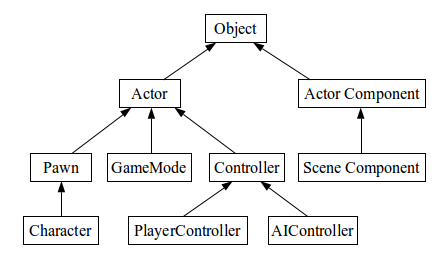
\includegraphics[width=0.75\textwidth]{Images/actor_component_diagram.png}
    \caption{Schema concettuale del paradigma Actor-Component in Unreal Engine: un singolo Attore funge da contenitore per logica, geometria e collisioni.}
    \label{fig:actor_component}
\end{figure}

%%%%%%%%%%%%%%%%%%%%%%%%%%%%%%%%%%%%%%%%%%%%%%%%%%%%%%%%%%%%%%%%%%%%%%%%%%%%%%%%%%%%%%%%%%%%%%%%%%%%%

\subsection{Il ciclo di vita degli oggetti e il sistema di Tick}
Il secondo elemento cruciale per la simulazione di sistemi dinamici è la discretizzazione e la gestione del tempo informatico. All'interno di Unreal Engine, il ciclo di vita di ogni Attore è scandito da metodi virtuali specifici che il programmatore può sovrascrivere (\textit{override}) in C++ per iniettare la logica matematica desiderata. I due metodi cardine su cui si basa l'integrazione numerica dell'intero simulatore sono \lstinline|BeginPlay()| e \lstinline|Tick()|.

L'inizializzazione del modello fisico avviene all'interno della funzione \lstinline|BeginPlay()|. Invocata una singola volta nell'esatto momento in cui l'Attore viene generato nello spazio (o al lancio della simulazione), questa funzione è deputata all'allocazione delle risorse di memoria, alla definizione delle masse strutturali a secco e, nel caso della vela solare, al calcolo istantaneo della velocità orbitale circolare necessaria a garantire la stabilità kepleriana di partenza, calcolando visivamente l'orbita di parcheggio.

Terminata la delicata fase di inizializzazione, il controllo passa alla funzione \lstinline|Tick(float DeltaTime)|, che rappresenta il vero cuore pulsante del \textit{solver} astrodinamico. A differenza dei solutori matematici statici che calcolano traiettorie predeterminate, il motore grafico opera tramite un ciclo continuo (il \textit{game loop}). Ad ogni fotogramma (\textit{frame}) renderizzato dalla scheda video, il motore invoca la funzione \lstinline|Tick| su tutti gli Attori attivi, fornendo come parametro di ingresso il \lstinline|DeltaTime| ($\Delta t$). Tale parametro rappresenta in modo rigoroso l'intervallo temporale, espresso in frazioni di secondo, trascorso dalla precedente esecuzione.

In ottica astrodinamica, il \lstinline|DeltaTime| assume il ruolo di passo di integrazione (il $dt$ delle equazioni differenziali ordinarie). Ad ogni singola esecuzione del \lstinline|Tick|, l'Attore \lstinline|ASolarSail| esegue sequenzialmente i seguenti calcoli computazionali:
\begin{enumerate}
    \item Interroga i propri componenti geometrici per ricalcolare l'area effettiva esposta al Sole ($A_{\text{eff}}$) basandosi sull'assetto istantaneo.
    \item Calcola la risultante vettoriale delle forze in gioco, sommando l'attrazione gravitazionale ($\mathbf{a}_g$) e la pressione di radiazione solare ($\mathbf{a}_{\text{SRP}}$).
    \item Integra le forze ricavando la nuova accelerazione netta, la quale viene moltiplicata per il \lstinline|DeltaTime| per ottenere la variazione di velocità vettoriale ($d\mathbf{v}$).
    \item Aggiorna la trasformazione spaziale 3D del veicolo in base alla nuova cinematica locale.
\end{enumerate}

\begin{figure}[htbp!]
    \centering
    % 
\includegraphics[width=0.8\textwidth]{Images/tick_physics_loop.png}
    \caption{Diagramma di flusso dell'integrazione numerica eseguita a ogni ciclo di \textit{Tick}: il motore grafico funge da solutore iterativo per le equazioni differenziali del moto.}
    \label{fig:tick_physics_loop}
\end{figure}

Questo approccio a ciclo continuo garantisce che la simulazione avvenga in modo fluido e interattivo, permettendo all'ingegnere di variare a \textit{runtime} l'inclinazione della vela solare e osservare istantaneamente come tali variazioni modifichino l'accelerazione netta e la conseguente traiettoria del veicolo fotonico.

%%%%%%%%%%%%%%%%%%%%%%%%%%%%%%%%%%%%%%%%%%%%%%%%%%%%%%%%%%%%%%%%%%%%%%%%%%%%%%%%%%%%%%%%%%%%%%%%%%%%%
%%%%%%%%%%%%%%%%%%%%%%%%%%%%%%%%%%%%%%%%%%%%%%%%%%%%%%%%%%%%%%%%%%%%%%%%%%%%%%%%%%%%%%%%%%%%%%%%%%%%%

\section{Progettazione Object-Oriented (OOP) del sistema}
La validità di un simulatore scientifico non risiede unicamente nell'accuratezza matematica delle sue equazioni, ma anche nella robustezza dell'infrastruttura software che le elabora e le espone all'utente. Per gestire l'intrinseca complessità dello scambio vettoriale di quantità di moto, dell'integrazione orbitale in doppia precisione e dell'avanzamento temporale, il codice C++ alla base dell'applicativo è stato strutturato seguendo rigorosamente i principi della Programmazione Orientata agli Oggetti (OOP). 

Questo approccio formale garantisce un'elevata coesione interna ai singoli moduli informatici e un basso accoppiamento (\textit{loose coupling}) tra le classi, favorendo la stabilità del simulatore, la sua facile manutenibilità e la futura espansione del progetto verso scenari interplanetari.

%%%%%%%%%%%%%%%%%%%%%%%%%%%%%%%%%%%%%%%%%%%%%%%%%%%%%%%%%%%%%%%%%%%%%%%%%%%%%%%%%%%%%%%%%%%%%%%%%%%%%

\subsection{Gerarchia delle classi e diagramma UML}
La progettazione della gerarchia delle classi parte dall'estensione delle entità base fornite dal framework di Unreal Engine, sfruttando pesantemente il sistema di riflessione nativo (\textit{Reflection System}) del motore tramite le macro C++ \lstinline|UCLASS()| e \lstinline|GENERATED_BODY()|. La struttura architetturale è riassumibile in due rami principali di esecuzione, che comunicano tra loro esclusivamente tramite riferimenti deboli (\textit{pointers}) e interfacce ben definite.



Come illustrato nel diagramma UML del sistema, le entità fondanti del simulatore derivano direttamente dalla superclasse \lstinline|AActor|:
\begin{itemize}
    \item \lstinline|ASimulationManager|: Progettato seguendo una logica operativa affine al \textit{Singleton pattern} (in quanto deve rigorosamente esisterne una sola istanza attiva nel livello simulato), questo Attore funge da orchestratore globale. Esso detiene il controllo centralizzato del tempo di simulazione (\lstinline|TimeScale|), calcola il vettore direzionale globale dell'illuminazione solare e gestisce l'inizializzazione del \textit{Data Logging} persistente. La sua esistenza solleva i singoli veicoli spaziali dal gravoso compito di dover recuperare autonomamente informazioni ambientali condivise.
    \item \textbf{Gerarchia del Veicolo:} La complessa rappresentazione della vela solare è interamente incapsulata nella classe \lstinline|ASolarSail|. A sua volta, per garantire un'alta specializzazione logica, la classe delega calcoli specifici a componenti software dedicati (derivati da \lstinline|UActorComponent|). Ad esempio, la geometria di impatto e i materiali ottici sono gestiti da componenti strutturali, mentre le vitali variabili di stato orbitale (vettore posizione, vettore velocità, massa a secco) sono mantenute e protette all'interno dell'Attore principale.
\end{itemize}

Questa divisione netta e gerarchica permette di istanziare molteplici oggetti \lstinline|ASolarSail| simultaneamente all'interno dello stesso scenario (ad esempio, per testare vele competitive con aree geometriche o coefficienti di riflettività diversi) sotto la rigorosa supervisione centralizzata di un unico \lstinline|ASimulationManager|, garantendo la perfetta coerenza temporale dell'intero \textit{framework}.

\begin{figure}[htbp!]
    \centering
    % \includegraphics[width=0.8\textwidth]{Images/uml_class_diagram.jpg}
    \caption{Diagramma UML semplificato dell'architettura software: il Simulation Manager orchestra il tempo globale, mentre le istanze Solar Sail gestiscono la cinematica locale.}
    \label{fig:uml_diagram}
\end{figure}

%%%%%%%%%%%%%%%%%%%%%%%%%%%%%%%%%%%%%%%%%%%%%%%%%%%%%%%%%%%%%%%%%%%%%%%%%%%%%%%%%%%%%%%%%%%%%%%%%%%%%

\subsection{Incapsulamento dei moduli fisici e disaccoppiamento}
Il principio informatico dell'incapsulamento è stato applicato in modo stringente durante tutto lo sviluppo per proteggere l'integrità dei dati fisici e prevenire l'insorgere di stati del sistema matematicamente incoerenti (come masse strutturali negative o coefficienti ottici sommati superiori a 1, che violerebbero la conservazione dell'energia). 

Le variabili di stato cruciali per l'integrazione differenziale sono esplicitamente dichiarate con modificatori di accesso \lstinline|private| o \lstinline|protected| all'interno degli \textit{header file} (\lstinline|.h|). L'accesso e la mutazione di tali variabili dall'esterno avvengono esclusivamente tramite metodi \textit{getter} e \textit{setter} specifici. Ad esempio, la richiesta utente di modifica dell'assetto o dell'area della vela durante l'esecuzione invoca automaticamente una routine di validazione interna che ricalcola istantaneamente l'area effettiva esposta ($A_{\text{eff}}$), garantendo che la fisica vettoriale del \lstinline|Tick| non operi mai su dati obsoleti o asincroni.

Un aspetto peculiare dell'incapsulamento in ambiente Unreal Engine è l'uso strategico della macro di serializzazione \lstinline|UPROPERTY|. Per permettere all'utente finale (l'ingegnere aerospaziale o l'operatore di missione) di configurare i parametri iniziali senza dover ricompilare il codice sorgente C++, le variabili chiave sono state esposte all'editor visivo tramite specificatori mirati:

\begin{lstlisting}[language=C++, caption={Esempio di incapsulamento ed esposizione sicura dei parametri fisici in C++}]
UPROPERTY(EditAnywhere, BlueprintReadWrite, Category="Solar Sail|Physics", 
          meta=(ClampMin="0.01", UIMin="0.01"))
double DryMass;

UPROPERTY(EditAnywhere, BlueprintReadWrite, Category="Solar Sail|Optical", 
          meta=(ClampMin="0.0", ClampMax="1.0"))
double SpecularReflectance;
\end{lstlisting}

\begin{figure}[htbp!]
    \centering
    % 
\includegraphics[width=0.6\textwidth]{Images/uproperty_editor.png}
    \caption{L'esposizione sicura delle variabili di stato tramite \lstinline|UPROPERTY|. L'interfaccia generata automaticamente dall'editor rispetta i vincoli matematici imposti dai metadati C++, impedendo l'inserimento di valori fisicamente invalidi.}
    \label{fig:uproperty_editor}
\end{figure}

L'utilizzo dei metadati di restrizione (\lstinline|ClampMin|, \lstinline|ClampMax|) direttamente all'interno della macro rappresenta una trasposizione informatica diretta dei vincoli fisici naturali: impone a livello di editor che la massa non sia mai pari a zero (evitando disastrose divisioni per zero nel calcolo dell'accelerazione $\mathbf{a} = \mathbf{F}/m$) e costringe i coefficienti ottici nel ristretto dominio logico $[0, 1]$.

Dal punto di vista della logica di esecuzione, il modulo di calcolo orbitale puro (gravitazione universale di Newton) è stato tenuto logicamente disaccoppiato dal modulo ottico perturbativo (\textit{ray casting} e pressione di radiazione fotonica). La funzione \lstinline|Tick()| invoca questi sottomoduli in stretta sequenza, accumulando le singole forze in un vettore \lstinline|NetForce| tridimensionale globale. Questo approccio altamente modulare assicura che in futuro sia possibile implementare nuove perturbazioni astrodinamiche (ad esempio, l'effetto dell'albedo terrestre, l'attrazione gravitazionale di un terzo corpo come la Luna o l'attrito atmosferico residuo per orbite LEO bassissime) semplicemente aggiungendo una nuova funzione matematica alla \textit{pipeline} di sommatoria delle forze, senza dover in alcun modo alterare o riscrivere il delicato nucleo del risolutore cinematico principale.

%%%%%%%%%%%%%%%%%%%%%%%%%%%%%%%%%%%%%%%%%%%%%%%%%%%%%%%%%%%%%%%%%%%%%%%%%%%%%%%%%%%%%%%%%%%%%%%%%%%%%
%%%%%%%%%%%%%%%%%%%%%%%%%%%%%%%%%%%%%%%%%%%%%%%%%%%%%%%%%%%%%%%%%%%%%%%%%%%%%%%%%%%%%%%%%%%%%%%%%%%%%

\section{Il gestore della simulazione (Simulation Manager)}
Il corretto e coerente svolgimento di una simulazione astrodinamica interattiva richiede un'entità di supervisione astratta che svincoli i singoli veicoli spaziali dalla complessa gestione dell'ambiente condiviso. In ottemperanza ai rigorosi principi di progettazione modulare precedentemente descritti, questo ruolo apicale è ricoperto dalla classe \lstinline|ASimulationManager|. 

Derivata direttamente da \lstinline|AActor| per poter esistere fisicamente all'interno del mondo virtuale, questa classe agisce come \textit{hub} centrale dell'applicativo, garantendo che tutti gli elementi vettoriali dello scenario siano perfettamente sincronizzati rispetto a un unico orologio globale e a un unico sistema di riferimento ambientale condiviso.

%%%%%%%%%%%%%%%%%%%%%%%%%%%%%%%%%%%%%%%%%%%%%%%%%%%%%%%%%%%%%%%%%%%%%%%%%%%%%%%%%%%%%%%%%%%%%%%%%%%%%

\subsection{Inizializzazione e controllo dello stato globale}
Il primo e più critico compito del gestore si esplica nella primissima fase di avvio (\lstinline|BeginPlay()|). Il \lstinline|ASimulationManager| è unico responsabile della validazione dello stato iniziale del mondo tridimensionale. Attraverso le potenti librerie di sistema fornite dal motore (come la funzione \lstinline|UGameplayStatics::GetAllActorsOfClass|), il gestore acquisisce automaticamente all'avvio i puntatori di memoria a tutte le istanze di tipo \lstinline|ASolarSail| correntemente presenti nel livello, costruendo un registro dinamico e aggiornato dei veicoli attivi. 

Questa rigida centralizzazione informativa è fondamentale per due aspetti cardine della simulazione fisica:
\begin{itemize}
    \item \textbf{Gestione univoca del vettore solare:} Invece di costringere ogni singola vela a ricalcolare pesantemente la posizione spaziale della sorgente luminosa a ogni \textit{Tick}, il \textit{Manager} interroga una singola volta la luce direzionale del livello (che agisce come \textit{proxy} del Sole) ed estrae il versore di propagazione vettoriale della luce ($\mathbf{u}$). Questo singolo vettore viene poi trasmesso a cascata, in modo estremamente efficiente, a tutte le vele solari registrate, garantendo un'assoluta coerenza ottica e geometrica in tutto lo spazio simulato.
    \item \textbf{Controllo autoritativo del TimeScale:} Il gestore detiene in esclusiva la variabile globale \lstinline|TimeScale|, che rappresenta il fattore numerico di dilatazione temporale. Nelle simulazioni di meccanica orbitale a spinta continua, dove una singola manovra di innalzamento orbitale può durare mesi effettivi, eseguire il programma in rapporto 1:1 rispetto alla realtà è ingegneristicamente inefficace. Il \textit{Manager} funge da \textit{time-keeper} assoluto, inoltrando costantemente il valore di \lstinline|TimeScale| ai sottomoduli fisici per scalare matematicamente il parametro \lstinline|DeltaTime| ($\Delta t$). Ciò permette l'esecuzione fluida della modalità accelerata (\textit{Accelerated Time Mode}) a livello logico, mantenendo però rigorosamente stabile il \textit{framerate} di rendering visivo per l'utente.
\end{itemize}

Inoltre, lo stato globale gestito centralmente include l'inizializzazione dei complessi flussi di I/O (Input/Output). Il \lstinline|ASimulationManager| apre all'avvio i canali di comunicazione per il \textit{Data Logging}, preparando e formattando i file CSV necessari per la registrazione periodica e persistente della telemetria orbitale, sollevando così la singola classe \lstinline|ASolarSail| dal gravoso onere informatico della gestione del \textit{file system} del sistema operativo ospite.

%%%%%%%%%%%%%%%%%%%%%%%%%%%%%%%%%%%%%%%%%%%%%%%%%%%%%%%%%%%%%%%%%%%%%%%%%%%%%%%%%%%%%%%%%%%%%%%%%%%%%

\subsection{Gestione della telecamera e degli input utente}
Affinché il simulatore sviluppato in Unreal Engine funga da strumento di indagine e validazione utile, l'ingegnere deve poter ispezionare visivamente il veicolo spaziale in ogni istante e alterare i parametri critici della missione a \textit{runtime}. Poiché la vela solare (\lstinline|ASolarSail|) è concettualmente un oggetto passivo, sottoposto unicamente a rigide leggi fisiche esterne, dotarla direttamente di logiche informatiche per la lettura periferica della tastiera o del mouse violerebbe il fondamentale principio architetturale di singola responsabilità (\textit{Single Responsibility Principle}).

Il \lstinline|ASimulationManager| (operando talvolta in concerto con un \lstinline|APawn| specializzato ad esso collegato, configurato come \textit{Player Controller}) si interfaccia quindi in modo esclusivo con il moderno sistema di input del motore (\textit{Enhanced Input System}), traducendo le azioni fisiche dell'utente in precisi comandi vettoriali per la simulazione:
\begin{itemize}
    \item \textbf{Interazione visiva orbitale:} La telecamera di osservazione non è rozzamente ancorata alla geometria della vela, ma è sofisticatamente vincolata tramite un \lstinline|USpringArmComponent|. Questo braccio virtuale flessibile agisce da perfetto giunto sferico matematico, permettendo all'utente di orbitare visivamente attorno al veicolo (tramite complessi movimenti di \textit{pan}, \textit{tilt} e \textit{zoom}) mantenendo il centro di massa dinamico della vela esattamente al centro dello schermo (\textit{focus point}), il tutto in modo totalmente indipendente dall'enorme velocità orbitale del mezzo spaziale simulato.
    
    \item \textbf{Alterazione dinamica dell'assetto e del tempo:} Attraverso specifiche mappature dei tasti configurate nel motore, l'utente può incrementare o decrementare istantaneamente il \lstinline|TimeScale| globale per navigare rapidamente e fluidamente nel tempo di missione. Parallelamente, gli input direzionali continui vengono catturati, filtrati e applicati per variare in tempo reale gli angoli di Eulero di beccheggio (\textit{pitch}) e imbardata (\textit{yaw}) della vela solare. 
\end{itemize}



Quando l'utente richiede una variazione di assetto spaziale, il \textit{Manager} invia il comando vettoriale alla vela, la quale, al primissimo ciclo di \lstinline|Tick| utile, ricalcolerà immediatamente il nuovo vettore normale $\mathbf{n}$ locale, la nuova e ridotta area effettiva esposta $A_{\text{eff}}$ e la conseguente variazione dell'accelerazione perturbativa fotonica. Questa catena di eventi informatici garantisce una responsività immediata dell'interfaccia visiva del simulatore, senza mai compromettere la stabilità o la precisione numerica dell'integrazione differenziale in corso in background.

\begin{figure}[htbp!]
    \centering
    % \includegraphics[width=0.85\textwidth]{Images/editor_input_camera.jpg}
    \caption{Visuale dall'editor del simulatore: il sistema di telecamera basato su \textit{SpringArm} permette di ispezionare il veicolo senza interferire con la cinematica orbitale locale.}
    \label{fig:editor_camera}
\end{figure}

%%%%%%%%%%%%%%%%%%%%%%%%%%%%%%%%%%%%%%%%%%%%%%%%%%%%%%%%%%%%%%%%%%%%%%%%%%%%%%%%%%%%%%%%%%%%%%%%%%%%%
%%%%%%%%%%%%%%%%%%%%%%%%%%%%%%%%%%%%%%%%%%%%%%%%%%%%%%%%%%%%%%%%%%%%%%%%%%%%%%%%%%%%%%%%%%%%%%%%%%%%%

\section{Modellazione del veicolo spaziale (Solar Sail)}
Se il \lstinline|ASimulationManager| rappresenta indubbiamente il "cervello" ambientale e temporale del simulatore, la complessa classe \lstinline|ASolarSail| ne costituisce il vero e proprio fulcro fisico e cinematico. Progettata ingegneristicamente come una specializzazione avanzata della classe base \lstinline|AActor|, questa entità informatica funge da "gemello digitale" (\textit{digital twin}) della sonda spaziale fisica. Il suo scopo informatico è intrinsecamente duplice: fornire una rappresentazione spaziale estremamente accurata per il calcolo delle delicate intersezioni ottiche fotoniche e incapsulare lo stato dinamico vettoriale del veicolo, evolvendolo coerentemente istante per istante.

%%%%%%%%%%%%%%%%%%%%%%%%%%%%%%%%%%%%%%%%%%%%%%%%%%%%%%%%%%%%%%%%%%%%%%%%%%%%%%%%%%%%%%%%%%%%%%%%%%%%%

\subsection{Rappresentazione geometrica e mesh poligonale}
La membrana riflettente della vela solare simulata non è trattata informaticamente come una semplice astrazione matematica puntiforme o monodimensionale, bensì come un corpo fisico esteso nello spazio tridimensionale interplanetario. Per modellare con fedeltà questa vasta estensione planare, la classe \lstinline|ASolarSail| impiega al suo interno un \lstinline|UStaticMeshComponent|, il quale ospita e renderizza la geometria tridimensionale del velivolo progettata tramite software CAD.

La scelta progettuale di utilizzare una complessa mesh poligonale invece di forme primitive analitiche è strettamente legata alle stringenti necessità degli algoritmi di calcolo della Pressione di Radiazione Solare (SRP). Dal punto di vista informatico e del \textit{rendering}, l'immensa superficie riflettente è discretizzata e composta da un vasto insieme di triangoli complanari. Questa discretizzazione geometrica avanzata offre vantaggi ingegneristici fondamentali:
\begin{itemize}
    \item \textbf{Estrazione immediata del Vettore Normale ($\mathbf{n}$):} Il motore grafico, essendo nativamente ottimizzato per il calcolo delle normali alle superfici, è in grado di calcolare istantaneamente il vettore matematico perpendicolare alla faccia dei soli poligoni correntemente illuminati. Questo versore dinamico è il parametro cardine indispensabile per l'applicazione della legge del coseno ottica ($A_{\text{eff}} = A \cos\alpha$) e per determinare la precisa direzione tridimensionale della forza risultante riflessa.
    \item \textbf{Collider avanzato per il Ray Casting:} La mesh poligonale non possiede una valenza unicamente estetica per l'operatore, ma agisce attivamente come un \textit{collider} matematico di precisione. Quando gli infiniti raggi (vettori direzionali continui) generati idealmente dal \textit{Simulation Manager} in direzione della vela intersecano fisicamente i poligoni virtuali, l'efficiente sistema di collisione interno di Unreal Engine restituisce una complessa struttura dati definita \lstinline|FHitResult|. Questa struttura software contiene informazioni numeriche esatte sul punto tridimensionale d'impatto e sull'orientamento spaziale esatto della micro-superficie colpita, permettendo all'algoritmo del simulatore di distinguere con precisione millimetrica tra un'illuminazione frontale pura, un'illuminazione radente inefficace o una condizione totale di ombra auto-indotta.
\end{itemize}

\begin{figure}[htbp!]
    \centering
    % 
\includegraphics[width=0.75\textwidth]{Images/sail_wireframe.png}
    \caption{Visualizzazione \textit{wireframe} (a fil di ferro) della membrana solare simulata in Unreal Engine. L'alta densità poligonale garantisce una discretizzazione spaziale eccellente per l'accuratezza degli algoritmi di \textit{Ray Casting}.}
    \label{fig:sail_wireframe}
\end{figure}

Infine, per garantire il massimo rigore sia visivo che prestazionale durante la simulazione in tempo reale, al componente geometrico principale viene applicato uno specifico \textit{Material Instance} dinamico programmato nel \textit{Material Graph} del motore. Questo \textit{material shader} fotorealistico è configurato rigorosamente in modalità \textit{Two-Sided} (doppia faccia fisica): un lato simula visivamente e computazionalmente il sottile film di alluminio altamente riflettente (su cui l'algoritmo calcola l'effettiva spinta propulsiva), mentre il lato opposto rappresenta il nudo polimero di supporto (es. Kapton o Mylar), caratterizzato da un'alta emissività termica e nullo potere propulsivo fotonico.

%%%%%%%%%%%%%%%%%%%%%%%%%%%%%%%%%%%%%%%%%%%%%%%%%%%%%%%%%%%%%%%%%%%%%%%%%%%%%%%%%%%%%%%%%%%%%%%%%%%%%

\subsection{L'abbandono della fisica nativa e l'integrazione numerica}
Affinché il modello geometrico tridimensionale precedentemente descritto si comporti coerentemente come un corpo fisico reale soggetto unicamente alle immani leggi della dinamica orbitale kepleriana, la classe \lstinline|ASolarSail| deve necessariamente essere arricchita con un esteso set di variabili di stato vettoriali e costanti strutturali, tutte opportunamente incapsulate e protette.

Il punto di svolta architetturale più critico di tutto il simulatore risiede nella deliberata scelta ingegneristica di **disattivare completamente** il motore fisico predefinito nativo di Unreal Engine (conosciuto come PhysX nelle vecchie versioni, o Chaos Physics nelle attuali). Tali motori commerciali di \textit{rigid body dynamics}, pur essendo eccellenti per simulare la gravità terrestre costante a livello del suolo o le collisioni tra automobili in un videogioco, sono informaticamente basati su approssimazioni a singola precisione (\lstinline|float|) e su solutori Euleriani elementari. Essi risultano totalmente inadeguati e imprecisi se scalati sulle enormi distanze interplanetarie, collassando vittima di devastanti errori di arrotondamento (\textit{floating-point underflow}) se applicati all'integrazione di orbite geocentriche.

Per bypassare questo limite commerciale, la classe \lstinline|ASolarSail| implementa da zero una propria rigorosa struttura dati cinematica personalizzata basata esclusivamente su primitive a **doppia precisione matematica** (a 64-bit). All'interno dell'Attore sono definiti i seguenti raggruppamenti logici di proprietà fisiche:
\begin{itemize}
    \item \textbf{Parametri Strutturali Nominali:} Includono la massa a secco in kg del \textit{payload} scientifico e dei pesanti bracci telescopici in fibra di carbonio, la massa specifica infinitesimale del film polimerico riflettente e l'area fisica totale nominale della vela ($A$). Questi rigidi valori vengono utilizzati unicamente durante la fase di \lstinline|BeginPlay| per calcolare e allocare in memoria la massa totale inerziale costante ($m$) del veicolo.
    \item \textbf{Coefficienti Ottici Realistici:} Variabili a virgola mobile a doppia precisione (rigorosamente vincolate tra i valori logici 0.0 e 1.0) che definiscono le precise percentuali di riflettività speculare pura ($\rho_s$), riflettività diffusa (\textit{scattering} lambertiano, $\rho_d$) e totale assorbimento termico ($\alpha_a$). Questo set di coefficienti permette all'operatore informatico di passare quasi istantaneamente da un modello di simulazione ideale teorico a uno altamente degradato o fotorealisticamente accurato.
    \item \textbf{Vettori Cinematici di Stato:} Per la corretta esecuzione dell'integrazione numerica discreta delle equazioni del moto di Newton, la classe mantiene costantemente instanziati in memoria RAM tre fondamentali vettori a doppia precisione (\lstinline|FVector3d| o \lstinline|FVector64| a seconda della build): l'assoluto vettore Posizione Globale $\mathbf{r}$ (rispetto al centro di massa del corpo attrattore planetario), l'istantaneo vettore Velocità orbitale $\mathbf{v}$ e la risultante vettoriale dell'accelerazione $\mathbf{a}$.
\end{itemize}

Durante l'esecuzione di ogni singolo e ravvicinato ciclo di \lstinline|Tick|, questi tre massicci gruppi di proprietà convergono in un'unica complessa operazione differenziale: l'area geometrica e i coefficienti ottici determinano il vettore della forza fotonica incidente; la massa strutturale permette di convertire immediatamente tale forza repulsiva in accelerazione vettoriale locale ($\mathbf{a} = \mathbf{F}/m$) sommandola al massiccio contributo gravitazionale dipendente dalla stringente posizione $\mathbf{r}$; infine, l'algoritmo di integrazione numerica personalizzato (che sarà approfonditamente discusso nel Capitolo 4) aggiorna matematicamente la nuova velocità $\mathbf{v}$ e la conseguente posizione spaziale orbitale.

Questa fusione profonda e inestricabile tra geometria pura (la mesh poligonale) e matematica avanzata (vettori a 64-bit e complessi coefficienti ottici) all'interno di un'unica classe C++ estremamente coesa, dimostra inequivocabilmente l'efficacia e l'assoluta necessità del paradigma \textit{Object-Oriented} nella moderna progettazione aerospaziale: il veicolo simulato è un'entità informatica autonoma, autosufficiente, che incapsula al proprio interno tutto l'hardware e il software di cui ha vitale bisogno per "subire" coerentemente le immani leggi dell'universo virtuale orchestrato dal Simulation Manager.

%%%%%%%%%%%%%%%%%%%%%%%%%%%%%%%%%%%%%%%%%%%%%%%%%%%%%%%%%%%%%%%%%%%%%%%%%%%%%%%%%%%%%%%%%%%%%%%%%%%%%
%%%%%%%%%%%%%%%%%%%%%%%%%%%%%%%%%%%%%%%%%%%%%%%%%%%%%%%%%%%%%%%%%%%%%%%%%%%%%%%%%%%%%%%%%%%%%%%%%%%%%
\chapter{Implementazione Fisica}
\label{chap:implementazione_fisica}

Dopo aver descritto nel capitolo precedente l'architettura del software, in questa sezione viene analizzata la logica fisica che permette al simulatore di funzionare. Se il capitolo precedente si è occupato della "struttura" del programma, questo si concentra su come le leggi fisiche vengano tradotte in algoritmi veri e propri. L’obiettivo principale è trasformare i modelli teorici presentati nel Capitolo 2 in istruzioni che il computer possa eseguire in tempo reale.

In questo contesto, Unreal Engine non viene utilizzato solo come motore grafico, ma come un vero e proprio solutore numerico. Il sistema deve infatti calcolare ogni forza agente sulla vela solare, dalla gravità terrestre alla spinta dei fotoni solari, per ottenere la forza totale che ne determina il movimento. Nelle sezioni che seguono verrà descritto l'intero schema di calcolo: dalla gestione delle unità di misura e delle condizioni iniziali, fino all'uso del \textit{ray casting} per simulare l'impatto della luce sulla superficie della vela.

%%%%%%%%%%%%%%%%%%%%%%%%%%%%%%%%%%%%%%%%%%%%%%%%%%%%%%%%%%%%%%%%%%%%%%%%%%%%%%%%%%%%%%%%%%%%%%%%
%%%%%%%%%%%%%%%%%%%%%%%%%%%%%%%%%%%%%%%%%%%%%%%%%%%%%%%%%%%%%%%%%%%%%%%%%%%%%%%%%%%%%%%%%%%%%%%%

\section{Dimensioni di riferimento}

Sviluppare un simulatore spaziale all'interno di Unreal Engine 5 richiede di superare un ostacolo tecnico importante: adattare un motore nato per i videogiochi a calcoli scientifici di alta precisione. Nativamente, infatti, la struttura di Unreal è pensata per gestire distanze e movimenti su scala "umana", dove tutto si misura in metri e centimetri.

Nello spazio profondo, al contrario, le distanze sono enormi. Il movimento di una sonda spaziale non può essere calcolato come quello di un normale personaggio 3D: a distanze astronomiche, gli errori di arrotondamento del computer si accumulerebbero a ogni singolo fotogramma (\textit{Tick}), compromettendo l'orbita in pochissimo tempo e portando all'alterazione della simulazione o al suo diretto fallimento. Per risolvere questo problema, il simulatore esegue i calcoli fisici "dietro le quinte", in cui le unità di misura vengono ricalibrate appositamente per le distanze interplanetarie.

\subsection{Il sistema di riferimento del simulatore}

In astrodinamica, le traiettorie vengono sempre calcolate prendendo come ancoraggio il corpo celeste principale attorno a cui si orbita. Poiché il simulatore è progettato per ancorare le vele solari alla Terra, l'architettura software adotta nativamente un sistema di riferimento geocentrico. Per tradurre questo concetto all'interno di Unreal Engine, il centro di massa della Terra viene fatto coincidere con l'origine tridimensionale del livello virtuale. Come definito all'interno della classe \lstinline|ASimulationManager|, la variabile \lstinline|EARTH_POSITION| è impostata alle coordinate $(0.0, 0.0, 0.0)$:

\begin{lstlisting}[language=C++, caption={Definizione delle coordinate centrali in \lstinline|SimulationManager.h|.}]
UPROPERTY(VisibleAnywhere, 
        Category = "Simulation Parameters | Bodies | Earth")
FVector3d EARTH_POSITION = FVector3d(0.0, 0.0, 0.0);

UPROPERTY(VisibleAnywhere,
        Category = "Simulation Parameters | Bodies | Sun")
FVector3d SUN_POSITION = FVector3d(149597870.7, 0.0, 0.0);
\end{lstlisting}

Questa configurazione crea un sistema di riferimento inerziale geocentrico. Il Sole viene invece posizionato lungo l'asse X alla sua distanza astronomica reale (circa 149 milioni di chilometri).

È importante precisare che posizionare la Terra esattamente al centro dell'universo virtuale è una scelta dettata da pura comodità logica e visiva. Il codice non è affatto vincolato in modo rigido all'origine del mondo: poiché l'intera architettura matematica è basata sul calcolo di vettori relativi (come la distanza tra la vela e \lstinline|EARTH_POSITION|), se al variare delle necessità di progetto si decidesse di spostare la Terra in un altro punto dello spazio, basterebbe aggiornarne le coordinate. Di conseguenza, tutti gli altri corpi coinvolti slitterebbero in modo coerente, mantenendo intatte le proporzioni e le leggi fisiche della simulazione.

\subsection{Scale astronomiche e necessità della doppia precisione}

Un motore grafico ragiona nativamente tramite unità di misura generiche definite "Unreal Units" (UU). Mantenere questa metrica anche per lo spazio profondo significherebbe costringere il calcolatore a gestire valori estremamente grandi, portando in breve tempo a errori di arrotondamento e alla perdita di stabilità dell'ambiente virtuale.

Per ovviare a questo ostacolo, all'interno del \lstinline|SimulationManager| è stata adottata una specifica convenzione di scala spaziale. Il sistema ricalibra le grandezze stabilendo che un chilometro di distanza nello spazio simulato corrisponda esattamente a 1000 unità del motore grafico:

\begin{lstlisting}[language=C++, caption={Fattori di scala per le distanze astronomiche in \lstinline|SimulationManager.h|.}]
UPROPERTY(VisibleAnywhere,
            Category = "Simulation Parameters | Unit Conversions")
float KM_TO_UU = 1000.0f;

UPROPERTY(VisibleAnywhere,
            Category = "Simulation Parameters | Unit Conversions")
float UU_TO_KM = 0.001f;
\end{lstlisting}

Attraverso questa proporzione, posizionare un satellite in orbita LEO a 400 km di quota si traduce in uno spostamento di 400.000 UU dal centro della terra, un valore numerico che il sistema è in grado di gestire in modo ottimale. 

Tuttavia, la sola gestione della scala spaziale non è sufficiente a garantire la stabilità orbitale. I vettori a singola precisione (\lstinline|float| a 32 bit) nativi del motore non sono in grado di identificare accuratamente variazioni millimetriche quando un corpo si trova a distanze di scala astronomica. Per far in modo di evitare eventuali deviazioni di traiettoria o errori di arrotondamento, l'intero sistema matematico del simulatore è basato su \lstinline|FVector3d|. L'implementazione della doppia precisione (\lstinline|double| a 64 bit) per le variabili di posizione rappresenta il requisito fondamentale e obbligatorio per operare in modo affidabile su distanze così grandi.

%%%%%%%%%%%%%%%%%%%%%%%%%%%%%%%%%%%%%%%%%%%%%%%%%%%%%%%%%%%%%%%%%%%%%%%%%%%%%%%%%%%%%%%%%%%%%%%%
%%%%%%%%%%%%%%%%%%%%%%%%%%%%%%%%%%%%%%%%%%%%%%%%%%%%%%%%%%%%%%%%%%%%%%%%%%%%%%%%%%%%%%%%%%%%%%%%

\section{Inizializzazione delle condizioni di partenza}

Affinché il solutore numerico possa calcolare correttamente l'evoluzione della traiettoria, è necessario definire con precisione lo stato fisico iniziale del veicolo al tempo zero ($t=0$). Questa fase preparatoria viene gestita dalla classe \lstinline|ASolarSail| attraverso una sequenza di funzioni di inizializzazione che si avviano automaticamente all'avvio della simulazione, all'interno dell'evento \lstinline|BeginPlay()|.

%%%%%%%%%%%%%%%%%%%%%%%%%%%%%%%%%%%%%%%%%%%%%%%%%%%%%%%%%%%%%%%%%%%%%%%%%%%%%%%%%%%%%%%%%%%%%%%%

\subsection{Collegamento al gestore globale}

La prima operazione è la funzione \lstinline|InitializeManager()|. Prima ancora di leggere la propria massa o posizione, la vela deve necessariamente agganciarsi all'istanza \textit{Singleton} del \lstinline|SimulationManager|; senza questo collegamento, la vela non avrebbe accesso alle costanti universali (come la massa della Terra o il fattore di scala \lstinline|KM_TO_UU|) e qualsiasi calcolo successivo genererebbe un errore. Una volta stabilito questo ponte comunicativo, è possibile procedere con il caricamento dei parametri fisici.

%%%%%%%%%%%%%%%%%%%%%%%%%%%%%%%%%%%%%%%%%%%%%%%%%%%%%%%%%%%%%%%%%%%%%%%%%%%%%%%%%%%%%%%%%%%%%%%%

\subsection{Parametrizzazione strutturale del veicolo}

Prima di poter elaborare qualsiasi forza attiva, il sistema deve caricare in memoria le proprietà fisiche e geometriche della vela. Questa operazione è delegata alla funzione \lstinline|InitializePhysicsProperties()|. I parametri fondamentali estratti dal pannello di controllo dell'utente sono due:

\begin{itemize}
    \item \textbf{Massa del veicolo ($m$):} Valore espresso in chilogrammi, essenziale per derivare l'accelerazione a partire dalla forza totale applicata, secondo il secondo principio della dinamica ($a = F/m$).
    \item \textbf{Area della vela ($A$):} Valore espresso in metri quadrati, che determina l'ampiezza della superficie esposta al flusso di fotoni. Maggiore è l'area, superiore sarà la spinta fotonica raccolta dal sistema.
\end{itemize}

Questi parametri, prelevati dall'interfaccia utente, vengono applicati direttamente al componente \lstinline|UStaticMeshComponent| (\lstinline|SAIL_MESH|), il quale rappresenta fisicamente la vela. In questo modo, l'algoritmo sovrascrive le impostazioni di default del motore per imporre i valori esatti richiesti dal modello matematico desiderato.

%%%%%%%%%%%%%%%%%%%%%%%%%%%%%%%%%%%%%%%%%%%%%%%%%%%%%%%%%%%%%%%%%%%%%%%%%%%%%%%%%%%%%%%%%%%%%%%%

\subsection{Collocamento geometrico e configurazione dell'orbita}

Una volta definita la struttura della vela, l'algoritmo deve posizionarla nello spazio. Questa operazione non si limita ad assegnare un semplice raggio orbitale predefinito, ma richiede di collocare il veicolo in un punto esatto lungo un'orbita tridimensionale. La funzione \lstinline|SetInitialPositions()| gestisce questa necessità unendo i parametri numerici della missione con il posizionamento spaziale stabilito visivamente nell'editor.

Per agevolare la configurazione rapida, il sistema usa un \lstinline|enum| (\lstinline|EOrbitStartType|) contenente i preset delle altitudini orbitali più comuni (come l'orbita LEO a 400 km o quella geostazionaria).

\begin{lstlisting}[language=C++, caption={Enumerazione dei preset orbitali nel file \lstinline|SolarSail.h|.}]
UENUM(BlueprintType)
enum class EOrbitStartType : uint8 {
    LEO_ISS       UMETA(DisplayName = "LEO (Stazione Spaziale - 400km)"),
    MEO_GPS       UMETA(DisplayName = "MEO (GPS - 20.200km)"),
    Geostationary UMETA(DisplayName = "GEO (Geostazionaria - 35.786km)"),
    LunarDistance UMETA(DisplayName = "Distanza Lunare (384.400km)"),
    CustomAltitude UMETA(DisplayName = "Altitudine Personalizzata")
};
\end{lstlisting}

Il sistema, tuttavia, non forza la comparsa della vela su un asse cartesiano predefinito. Al contrario, il codice rileva le coordinate in cui l'utente ha posizionato manualmente la vela all'interno della scena di Unreal (\lstinline|EditorLocation|) e calcola un versore (\lstinline|RadialDir|) che parte dal centro della Terra e punta esattamente in quella direzione. 

\begin{lstlisting}[language=C++, caption={Calcolo della posizione e della distanza radiale in \lstinline|SolarSail.cpp|.}]
FVector3d EditorLocation = FVector3d(GetActorLocation()); 
FVector3d EarthPosUU = Manager->EARTH_POSITION * Manager->KM_TO_UU;

// Calcolo della direzione in base al posizionamento nell'editor
FVector3d RadialDir = (EditorLocation - EarthPosUU).GetSafeNormal();

// Controllo di sicurezza per evitare vettori nulli
if (RadialDir.IsNearlyZero()) {
    RadialDir = FVector3d(1, 0, 0); 
}
\end{lstlisting}

Una volta stabilita la direzione, l'algoritmo estrae l'altitudine richiesta dal valore scelto dall'utente nell editor e vi somma il raggio equatoriale terrestre, ottenendo la distanza radiale reale dal centro di massa del pianeta. Questo valore viene convertito nelle unità di misura del motore grafico (\lstinline|TargetOrbitRadiusUU|) e moltiplicato per il versore direzionale. 

\begin{lstlisting} [language=C++, caption={Calcolo del raggio orbitale in \lstinline|SolarSail.cpp|.}]
double TargetOrbitRadiusKm = SelectedAltitudeKm + Manager->EARTH_RADIUS;
double TargetOrbitRadiusUU = TargetOrbitRadiusKm * Manager->KM_TO_UU;
FVector3d NewLocationUU = EarthPosUU + (RadialDir * TargetOrbitRadiusUU);
\end{lstlisting}

A questo punto, il calcolo matematico deve essere tradotto in un'azione all'interno dell'ambiente virtuale di Unreal. Tramite l'istruzione \lstinline|SetActorLocation()|, il software sposta fisicamente il modello 3D della vela alle nuove coordinate appena ottenute (\lstinline|NewLocationUU|). Contemporaneamente, le variabili di stato che rappresentano la posizione della vela e la distanza dal centro della Terra vengono aggiornate con i nuovi valori:

\begin{lstlisting}[language=C++, caption={Assegnazione delle coordinate e delle variabili di stato in \lstinline|SolarSail.cpp|.}]
// Spostamento fisico dell'attore nella scena
SetActorLocation(FVector(NewLocationUU));

// Inizializzazione delle variabili per il solutore fisico
SailPosition = NewLocationUU; 
OrbitRadius = TargetOrbitRadiusKm;
SailDistanceFromEarth = OrbitRadius;
\end{lstlisting}

Conservare in memoria questi valori (in particolar modo \lstinline|SailDistanceFromEarth|) è fondamentale: senza di essi, infatti, il motore fisico non avrebbe i dati di partenza per poter calcolare la forza gravitazionale e la spinta solare nel momento di inizio della simulazione.

Più semplicemente, l'algoritmo non stravolge la scena costruita dall'utente, ma la regolarizza. Il sistema guarda in che direzione è stata piazzata la vela nell'editor e si limita a "spingerla" lungo quella linea immaginaria, allontanandola, o avvicinandola, finché non raggiunge l'altitudine impostata. 

È stato inoltre inserito un meccanismo di emergenza: se per errore la vela venisse posizionata al centro della Terra (coordinate $0.0, 0.0, 0.0)$, il software non saprebbe in quale direzione allontanarla, poiché la distanza risulterebbe zero. Per evitare che questo errore matematico faccia andare in \textit{crash} il programma, l'algoritmo sposta la vela lungo l'asse X, garantendo un avvio sicuro della simulazione.

\begin{lstlisting}[language=C++, caption={Meccanismo di sicurezza per posizionamento errato in \lstinline|SolarSail.cpp|.}]
if (RadialDir.IsNearlyZero()) {
    RadialDir = FVector3d(1, 0, 0); 
}
\end{lstlisting}

%%%%%%%%%%%%%%%%%%%%%%%%%%%%%%%%%%%%%%%%%%%%%%%%%%%%%%%%%%%%%%%%%%%%%%%%%%%%%%%%%%%%%%%%%%%%%%%%

\subsection{Correzione dell'assetto e allineamento orbitale}

Posizionare la vela alla giusta distanza dalla Terra non basta. Affinché un'orbita circolare sia stabile sin dal primo istante, la spinta iniziale deve essere rigorosamente perpendicolare all'attrazione gravitazionale (ovvero a 90 gradi rispetto al raggio che unisce la vela al centro del pianeta). 

Poiché il simulatore permette all'utente di orientare liberamente la vela nell'editor grafico prima dell'avvio, è altamente probabile che la direzione scelta manualmente non sia una tangente perfetta. Anche un errore umano di frazioni di grado nell'inclinazione del modello 3D comporterebbe una componente di velocità radiale indesiderata, trasformando l'orbita circolare in un'ellisse o, nel peggiore dei casi, portando la vela a schiantarsi.

Per prevenire questo problema, prima di applicare qualsiasi forza, il sistema esegue la funzione \lstinline|SetInitialRotations()|, che si occupa di "raddrizzare" l'assetto del veicolo. L'algoritmo confronta la direzione verticale della vela (l'asse Z, scelto dall'utente) con la direzione radiale esatta della gravità terrestre (\lstinline|RadialDir|). Tramite un prodotto scalare (\lstinline|DotProduct|), il sistema calcola la porzione del vettore utente che sta accidentalmente puntando verso o contro la Terra, e la sottrae dal vettore originale:

\begin{lstlisting}[language=C++, caption={Correzione vettoriale della rotazione iniziale in \texttt{SolarSail.cpp}.}]
// Estrazione asse Z impostato dall'utente
FVector3d UserForward = FVector3d(GetActorUpVector());

// Calcolo della componente errata lungo il raggio e sua sottrazione
double RadialComponent = FVector3d::DotProduct(UserForward, RadialDir);
FVector3d ValidTangentDir = UserForward - (RadialDir * RadialComponent);
\end{lstlisting}

Il risultato, \lstinline|ValidTangentDir|, è un vettore puramente tangenziale all'orbita. A questo punto, il codice ricostruisce la matrice di rotazione dell'oggetto (\lstinline|FRotationMatrix::MakeFromZX|) e costringe il modello 3D della vela a ruotare (\lstinline|SetActorRotation|), allineando in modo impeccabile il suo asse Z alla nuova tangente calcolata. 

\begin{lstlisting}[language=C++, caption={Allineamento dell'assetto alla tangente orbitale in \texttt{SolarSail.cpp}.}]
FRotator NewRotation = FRotationMatrix::MakeFromZX((FVector)ValidTangentDir, (FVector)UserUpRef).Rotator();
    
SetActorRotation(NewRotation);
\end{lstlisting}

Anche in questo caso è previsto un meccanismo di sicurezza: se la vela fosse stata orientata dall'utente esattamente verso il centro della Terra, la sottrazione genererebbe un vettore nullo. In tal caso il sistema sceglie arbitrariamente di allineare la vela lungo l'asse X, garantendo comunque un assetto tangenziale corretto e un avvio stabile della simulazione.

\begin{lstlisting}[language=C++, caption={Meccanismo di sicurezza per assetto errato in \texttt{SolarSail.cpp}.}]
if (ValidTangentDir.IsNearlyZero()) {
    ValidTangentDir = FVector3d::CrossProduct(RadialDir, 
                                              FVector3d(1, 0, 0));
    if (ValidTangentDir.IsNearlyZero()) {
        ValidTangentDir = FVector3d(0, 1, 0);
    }
}
\end{lstlisting}

%%%%%%%%%%%%%%%%%%%%%%%%%%%%%%%%%%%%%%%%%%%%%%%%%%%%%%%%%%%%%%%%%%%%%%%%%%%%%%%%%%%%%%%%%%%%%%%%

\subsection{Calcolo e attribuzione della velocità orbitale iniziale}

Ancora una volta le modifiche strutturali applicate alla vela non sono sufficienti. Se la vela venisse semplicemente "rilasciata" in orbita con velocità nulla, l'attrazione gravitazionale terrestre la farebbe precipitare verso il centro del pianeta al primo istante di simulazione. Per mantenere la vela in un'orbita stabile, è indispensabile conferirle una velocità di lancio iniziale, in modo che la forza centrifuga bilanci l'attrazione gravitazionale.

Questa operazione viene eseguita dalla funzione \lstinline|SetInitialVelocity()|. L'algoritmo calcola innanzitutto il modulo (l'intensità) della velocità necessaria, sfruttando la formula classica della meccanica orbitale:

\begin{equation}
    v = \sqrt{\frac{G \cdot M}{r}}
\end{equation}

Dove:
\begin{itemize}
    \item $G$ è la costante di gravitazione universale, definita come \lstinline|GRAVITATIONAL_CONSTANT|.
    \item $M$ è la massa della Terra, definita come \lstinline|EARTH_MASS|.
    \item $r$ è la distanza radiale della vela dal centro della Terra, convertita in metri e ottenuta dalla variabile \lstinline|SailDistanceFromEarth|, precedentemente calcolata durante l'inizializzazione della posizione.
\end{itemize}

Tuttavia, il motore fisico di Unreal Engine richiede un vettore direzionale tridimensionale, non un semplice numero scalare. Essendo l'assetto della vela appena stato corretto e forzato sulla tangente orbitale (come descritto nel paragrafo precedente tramite la funzione \lstinline|SetInitialRotation()|), l'algoritmo non ha bisogno di eseguire ulteriori calcoli per stabilire la direzione in cui deve essere applicata la velocità orbitale iniziale. La direzione di lancio viene semplicemente estratta dall'asse verticale (l'asse Z locale, o "Up Vector") dell'attore tramite l'istruzione \lstinline|GetActorUpVector()|. 

Una volta ottenuto questo versore direzionale il sistema lo moltiplica per il modulo \lstinline|InitialOrbitVelocityModule| calcolato in precedenza per ottenere così il vettore della velocità iniziale.

Infine, tramite la funzione \lstinline|SetPhysicsLinearVelocity()|, la velocità calcolata viene passata direttamente al motore fisico di Unreal, imprimendo alla sonda la spinta meccanica reale per farla partire. In questo modo, l'oggetto entra a far parte a tutti gli effetti del sistema dinamico gestito dal motore.

\begin{lstlisting}[language=C++, caption={Calcolo e assegnazione della velocità orbitale iniziale in \lstinline|SolarSail.cpp|.}]
// Calcolo della distanza in metri con soglia di sicurezza
double Dist = FVector3d::Distance(CurrentPos, EarthPosUU) * Manager->UU_TO_METERS;
if (Dist < 1000.0) {
    Dist = 1000.0;
}

// Calcolo del modulo della velocita' orbitale
InitialOrbitVelocityModule = FMath::Sqrt((Manager->GRAVITATIONAL_CONSTANT * Manager->EARTH_MASS) / Dist);

// Estrazione della direzione di lancio
InitialOrbitVelocityVersor = FVector3d(GetActorUpVector());

// Calcolo del vettore finale
InitialOrbitVelocity = InitialOrbitVelocityVersor * InitialOrbitVelocityModule;

// Assegnazione della velocita' al motore fisico di Unreal
if(SAIL_MESH->IsSimulatingPhysics()) {
    SAIL_MESH->SetPhysicsLinearVelocity(FVector(InitialOrbitVelocity));
}
\end{lstlisting}

%%%%%%%%%%%%%%%%%%%%%%%%%%%%%%%%%%%%%%%%%%%%%%%%%%%%%%%%%%%%%%%%%%%%%%%%%%%%%%%%%%%%%%%%%%%%%%%%

\subsection{Inizializzazione della telemetria e delle condizioni di partenza}

Dopo aver posizionato la vela, averne corretto l'assetto e averle conferito la giusta velocità iniziale, la vela è fisicamente pronta per iniziare a orbitare. L'ultima istruzione eseguita dal \lstinline|BeginPlay()| non riguarda la dinamica della vela, ma la preparazione al salvataggio dei dati persistenti.

Qualora l'utente abbia abilitato la registrazione dei dati, l'esecuzione della funzione \lstinline|InitializeCSVReporting()| prepara il terreno per l'analisi della missione. In questa fase il sistema non elabora ancora alcuna dinamica, ma prepara l'ambiente di lavoro sul disco, creando le cartelle di destinazione e generando un file univoco per la vela (ad esempio \textit{SolarSailData\_Sail\_1.csv}). Il vero pregio di questa impostazione è la sua scalabilità nativa: se la simulazione prevede il lancio simultaneo di un'intera flotta di vele, il codice lo rileva e inizializza in automatico un file di telemetria dedicato per ogni singolo veicolo.

In questa fase il sistema si limita a preparare i file e a resettare i flag di scrittura (\lstinline|bCsvHeaderWritten|); la vera registrazione dei parametri fisici iniziali e la scrittura dell'intestazione (\textit{header}) avverranno in automatico durante la prima chiamata della funzione \lstinline|AppendDataToCSV| al primo frame utile della simulazione. Lo schema di salvataggio dei dati persistenti e l'analisi della telemetria di debug verranno approfonditi nel Capitolo 5.

%%%%%%%%%%%%%%%%%%%%%%%%%%%%%%%%%%%%%%%%%%%%%%%%%%%%%%%%%%%%%%%%%%%%%%%%%%%%%%%%%%%%%%%%%%%%%%%
%%%%%%%%%%%%%%%%%%%%%%%%%%%%%%%%%%%%%%%%%%%%%%%%%%%%%%%%%%%%%%%%%%%%%%%%%%%%%%%%%%%%%%%%%%%%%%%

\section{Modellazione della gravità terrestre}

Conclusa la fase di inizializzazione, il simulatore entra nel suo ciclo vitale: l'aggiornamento continuo a ogni fotogramma (\textit{Tick}). Da questo momento in poi, il moto della vela non è più un semplice parametro preimpostato, ma è governato dall'interazione dinamica delle forze in gioco. La più importante e costante di queste è senza dubbio l'attrazione gravitazionale terrestre.

Per mantenere l'architettura del software pulita ed efficiente, l'elaborazione di questa dinamica è stata suddivisa in due passaggi logici: il calcolo matematico (affidato al sistema centrale \lstinline|SimulationManager|) e l'applicazione meccanica (gestita dal singolo veicolo \lstinline|SolarSail|).

%%%%%%%%%%%%%%%%%%%%%%%%%%%%%%%%%%%%%%%%%%%%%%%%%%%%%%%%%%%%%%%%%%%%%%%%%%%%%%%%%%%%%%%%%%%%%%%

\subsection{Calcolo vettoriale dell'accelerazione di gravità}

La funzione \lstinline|GetEarthGravityAccelerationAt()|, contenuta nel \lstinline|SimulationManager|, funge da calcolatrice universale per l'intero sistema. Il suo scopo è determinare l'esatta accelerazione di gravità in un qualsiasi punto dello spazio virtuale.

L'algoritmo parte dalla formulazione classica della legge di gravitazione universale di Newton, riadattata per trovare l'accelerazione ($g$):

\begin{equation}
g = \frac{G \cdot M}{r^2}
\end{equation}

Dove:
\begin{itemize}
    \item $G$ è la costante di gravitazione universale, definita come \lstinline|GRAVITATIONAL_CONSTANT| e convertita in metri cubi al secondo quadrato per chilogrammo.
    \item $M$ è la massa della Terra, definita come \lstinline|EARTH_MASS| e anch'essa espressa in chilogrammi.
    \item $r$ è la distanza radiale della vela dal centro della Terra, espressa in metri e calcolata a partire dalla distanza in chilometri (\lstinline|DistanceFromEarthKm|) fornita come parametro di ingresso alla funzione.
\end{itemize}

Prima di eseguire il calcolo, il codice converte la distanza dal centro della Terra ($r$) in metri, un passaggio obbligatorio poiché la costante gravitazionale $G$ opera su questa specifica unità di misura. Ottenuto quindi il modulo dell'accelerazione (\lstinline|GravityAccelerationMagnitude|), il sistema necessita di un versore per orientare la forza nel mondo tridimensionale di Unreal Engine. 

L'algoritmo genera quindi un vettore direzionale normalizzato (\lstinline|DirectionToEarth|) che parte dalla posizione della sonda e punta dritto verso le coordinate terrestri. Moltiplicando questo versore per il modulo $g$, si ottiene il risultato finale: un vettore tridimensionale che indica al motore grafico non solo l'intensità dell'attrazione gravitazionale, ma anche la direzione verso la quale la vele viene attratta.

\begin{lstlisting}[language=C++, caption={Calcolo dell'accelerazione gravitazionale in \texttt{SimulationManager.cpp}.}]
double DistanceFromEarthM = DistanceFromEarthKm * 1000.0;

// Calcolo del modulo dell'accelerazione (g = GM/r^2)
double GravityAccelerationMagnitude = (GRAVITATIONAL_CONSTANT * EARTH_MASS) / (DistanceFromEarthM * DistanceFromEarthM);

// Vettore direzionale verso la Terra
FVector3d DirectionToEarth = (EARTH_POSITION - (SailLocationUU * UU_TO_KM)).GetSafeNormal();

return DirectionToEarth * GravityAccelerationMagnitude;
\end{lstlisting}

%%%%%%%%%%%%%%%%%%%%%%%%%%%%%%%%%%%%%%%%%%%%%%%%%%%%%%%%%%%%%%%%%%%%%%%%%%%%%%%%%%%%%%%%%%%%%%%

\subsection{Applicazione della forza e aggiornamento dinamico}

Mentre il Manager si occupa della teoria matematica, la classe \lstinline|ASolarSail| deve tradurre quei calcoli in vero movimento. Ad ogni singolo \textit{tick}, la vela richiama la funzione \lstinline|UpdateGravityForce()|. 

La specifica vela consulta il Manager (\lstinline|SimulationManager|) passandogli la propria posizione e ottiene in risposta il vettore dell'accelerazione appena calcolato. Applicando il secondo principio della dinamica ($F = m \cdot a$), l'algoritmo lo moltiplica per la massa del veicolo (\lstinline|SAIL_MASS|), ricavando la forza gravitazionale vera e propria, espressa in Newton.

A questo punto, la forza viene inserita nel motore fisico di Unreal tramite la funzione nativa \lstinline|AddForce()|.
Mentre la velocità di lancio è stata assegnata una sola volta come valore iniziale, \lstinline|AddForce| esercita un'attrazione ininterrotta. Ad ogni \textit{tick}, questa istruzione attira la sonda verso il centro del pianeta, agendo come forza centripeta per bilanciare l'inerzia del veicolo e mantenerlo costantemente vincolato alla sua orbitale.

\begin{lstlisting}[language=C++, caption={Applicazione dinamica della forza gravitazionale in \lstinline|SolarSail.cpp|.}]
// Richiesta dell'accelerazione al Manager
FVector3d GravityAccel = Manager->GetEarthGravityAccelerationAt(SailPosition, SailDistanceFromEarth);

// F = m * a
GravityForce = GravityAccel * SAIL_MASS;

// Applicazione continua della forza al motore fisico (se nei limiti di tempo)
if(Manager->TimeScale <= 1.1f) {
    if(SAIL_MESH->IsSimulatingPhysics()) {
        SAIL_MESH->AddForce(FVector(GravityForce));
    }
}
\end{lstlisting}

È importante sottolineare un limite di sicurezza fondamentale imposto in questa funzione: l'uso del comando nativo \lstinline|AddForce| è consentito solo se il tempo scorre a velocità quasi reale (\lstinline|TimeScale <= 1.1f|). I motori fisici, come \textit{Chaos Physics} per Unreal Engine, calcolano il movimento per ogni fotogramma. Se l'utente accelerasse la simulazione in modo estremo, lo spazio percorso dalla sonda tra un calcolo e l'altro diventerebbe troppo ampio: invece di descrivere una curva orbitale fluida, il veicolo procederebbe su lunghe rette, finendo per 'allargare' inesorabilmente la traiettoria e fuggire dall'orbita. Per evitare questo grave errore matematico, la fisica di Unreal viene sfruttata solo quando la densità dei calcoli garantisce una simulazione stabile.

%%%%%%%%%%%%%%%%%%%%%%%%%%%%%%%%%%%%%%%%%%%%%%%%%%%%%%%%%%%%%%%%%%%%%%%%%%%%%%%%%%%%%%%%%%%%%%%%
%%%%%%%%%%%%%%%%%%%%%%%%%%%%%%%%%%%%%%%%%%%%%%%%%%%%%%%%%%%%%%%%%%%%%%%%%%%%%%%%%%%%%%%%%%%%%%%%

\section{Il Campo di Pressione Solare (SRP)}

Accanto all'attrazione gravitazionale, la seconda componente fondamentale per la simulazione è la Pressione di Radiazione Solare (\textit{Solar Radiation Pressure}). Al contrario della gravità, che agisce sul centro di massa del veicolo, la pressione solare è una forza che agisce su tutta la superficie della vela ed è generata dall'impatto dei fotoni contro di essa. 

Mantenendo la coerenza strutturale definita al paragrafo precedente, anche il calcolo di questa interazione è stato separato in due parti logiche distinte: il calcolo della pressione di radiazione vera e propria (gestita centralmente dal \lstinline|SimulationManager|) e il calcolo della forza risultante sull'oggetto (delegata invece a \lstinline|SolarSail|).

%%%%%%%%%%%%%%%%%%%%%%%%%%%%%%%%%%%%%%%%%%%%%%%%%%%%%%%%%%%%%%%%%%%%%%%%%%%%%%%%%%%%%%%%%%%%%%%%

\subsection{Calcolo della distanza Vela-Sole}

L'intensità della radiazione solare non è costante, ma dipende strettamente dalla posizione della vela rispetto alla posizione del Sole. Pertanto, il primo valore necessario all'algoritmo per quantificare la spinta dei fotoni è la distanza tra il veicolo e la fonte luminosa.

All'interno della funzione \lstinline|GetSolarPressureAt()|, situata all'interno del gestore centrale \lstinline|SimulationManager|, il codice esegue per prima cosa una verifica sui parametri in ingresso. Il sistema controlla se la distanza radiale dal Sole (\lstinline|SailDistanceFromSunKm|) è già stata calcolata e fornita dalla vela che la richiama. In caso contrario (valore nullo o negativo), il Manager provvede a calcolarla autonomamente.

L'operazione viene eseguita misurando la distanza vettoriale tra le coordinate della vela (\lstinline|SailLocationUU|) e la posizione fissa del Sole (\lstinline|SUN_POSITION|), precedentemente scalata nelle unità di misura del motore grafico. Il risultato viene poi subito riconvertito in chilometri tramite il fattore \lstinline|UU_TO_KM|, mantendo lo schema di unità coerente con il resto del sistema.

%%%%%%%%%%%%%%%%%%%%%%%%%%%%%%%%%%%%%%%%%%%%%%%%%%%%%%%%%%%%%%%%%%%%%%%%%%%%%%%%%%%%%%%%%%%%%%%%

\subsection{La Legge del Quadrato Inverso applicata ai fotoni}

Una volta ottenuta la distanza su cui si trova la vela rispetto al Sole, l'algoritmo procede al calcolo effettivo della pressione di radiazione. La propagazione dell'energia luminosa nel vuoto è regolata dalla legge dell'inverso del quadrato: man mano che i fotoni si allontanano dalla stella, si distribuiscono su una superficie sferica sempre più ampia, causando un decadimento quadratico dell'intensità.

Il codice implementa questo principio fisico attraverso la formula standard per il calcolo della pressione solare ($P$):

\begin{equation}
    P = \frac{L}{4 \pi r^2 c}
\end{equation}

Dove:
\begin{itemize}
    \item $L$ è la luminosità solare, definita come \lstinline|SOLAR_LUMINOSITY| ($3.828 \times 10^{26} \, W$).
    \item $r$ è la distanza radiale dal Sole, definita come \lstinline|DistanceFromSunKm| convertita in metri.
    \item $c$ è la velocità della luce nel vuoto, definita come \lstinline|SPEED_OF_LIGHT| e convertita in metri al secondo.
\end{itemize}

Per fare in modo di essere il più coerenti possibile alle costanti fisiche (espresse nel Sistema Internazionale), il codice converte automaticamente la distanza \lstinline|DistanceFromSunKm| in metri prima di eseguire la divisione. Il risultato di questa operazione è un valore scalare espresso in Pascal ($N/m^2$), che rappresenta l'esatta pressione esercitata dalla luce in quel preciso punto dello spazio.

\begin{lstlisting}[language=C++, caption={Calcolo della Pressione Solare nel \lstinline|SimulationManager.cpp|.}]
double ASimulationManager::GetSolarPressureAt(FVector3d SailLocationUU, double SailDistanceFromSunKm) const {
    // Risoluzione della distanza in Chilometri
    double DistanceFromSunKm = SailDistanceFromSunKm > 0.0 ? SailDistanceFromSunKm : FVector3d::Distance(SailLocationUU, SUN_POSITION * KM_TO_UU) * UU_TO_KM;
    
    // Conversione obbligatoria in Metri per l'analisi dimensionale
    double DistanceFromSunM = DistanceFromSunKm * 1000.0;
    
    // P = L / (4 * PI * r^2 * c)
    double SolarPressure = SOLAR_LUMINOSITY / (4.0 * PI_GREEK * DistanceFromSunM * DistanceFromSunM * (SPEED_OF_LIGHT * 1000.0));
    
    return SolarPressure * ForceMultiplier;
}
\end{lstlisting}

%%%%%%%%%%%%%%%%%%%%%%%%%%%%%%%%%%%%%%%%%%%%%%%%%%%%%%%%%%%%%%%%%%%%%%%%%%%%%%%%%%%%%%%%%%%%%%%%

\subsection{Ottimizzazione del calcolo della pressione solare}

Delegare il calcolo di questa formula al \lstinline|SimulationManager| non è solo una questione di ordine nel codice, ma una scelta logica ben precisa. La pressione solare, infatti, è un dato ambientale universale: in questa fase dipende esclusivamente dalla distanza, a prescindere dall'inclinazione, dal materiale o dalla grandezza della vela che la riceve.

Mantenendo questa separazione logica, il sistema assicura che il Manager si comporti come un vero e proprio "fornitore" per quanto riguarda la pressione solare. Quando la classe \lstinline|ASolarSail| richiamerà questa funzione per calcolare la propria spinta, riceverà un valore di pressione pronto per i prossimi calcoli di forza.

\subsection{Alterazione controllata delle forze con \textit{Force Multiplier}}

Inoltre, questa struttura centralizzata permette l'inserimento di variabili di controllo globali, come il \lstinline|ForceMultiplier|. Moltiplicando il risultato finale per questo fattore esposto all'utente, il sistema offre la possibilità di aumentare o diminuire artificialmente l'intensità della luce solare per scopi di testing. Essendo inserito all'interno del Manager, questo moltiplicatore influenzerà coerentemente tutte le sonde presenti nella simulazione, senza richiedere modifiche successive ai calcoli locali delle singole vele.

%%%%%%%%%%%%%%%%%%%%%%%%%%%%%%%%%%%%%%%%%%%%%%%%%%%%%%%%%%%%%%%%%%%%%%%%%%%%%%%%%%%%%%%%%%%%%%%%
%%%%%%%%%%%%%%%%%%%%%%%%%%%%%%%%%%%%%%%%%%%%%%%%%%%%%%%%%%%%%%%%%%%%%%%%%%%%%%%%%%%%%%%%%%%%%%%%

\section{Lo schema ottico della Membrana}

Una volta calcolata la pressione ambientale esercitata dalla radiazione solare, il simulatore deve determinare come questa energia si traduca in vera e propria spinta meccanica per la vela. L'interazione tra i fotoni e il veicolo solare non è un semplice urto anelastico: il trasferimento di quantità di moto dipende in maniera diretta dalle proprietà ottiche e dai materiali di cui è composta la membrana.

%%%%%%%%%%%%%%%%%%%%%%%%%%%%%%%%%%%%%%%%%%%%%%%%%%%%%%%%%%%%%%%%%%%%%%%%%%%%%%%%%%%%%%%%%%%%%%%%

\subsection{Scomposizione dell'interazione fotone-superficie}

Nella realtà astrodinamica, quando un flusso di fotoni colpisce una superficie, la sua energia viene frammentata in tre fenomeni ottici primari:
\begin{itemize}
    \item \textbf{Assorbimento ($\alpha$):} Il fotone viene catturato dal materiale, cedendo la sua intera quantità di moto ma generando calore.
    \item \textbf{Riflessione speculare ($\rho_s$):} Il fotone rimbalza sulla superficie con un angolo di uscita identico a quello di ingresso, fornendo una spinta extra grazie al principio di azione e reazione.
    \item \textbf{Riflessione diffusa ($\rho_d$):} Il fotone rimbalza, ma a causa dell'irregolarità del materiale viene disperso in una direzione casuale, riducendo l'efficienza della spinta.
\end{itemize}

%%%%%%%%%%%%%%%%%%%%%%%%%%%%%%%%%%%%%%%%%%%%%%%%%%%%%%%%%%%%%%%%%%%%%%%%%%%%%%%%%%%%%%%%%%%%%%%%

\subsection{Parametrizzazione dei Coefficienti Ottici}

Per ottimizzare il sistema, il modello matematico condensa queste proprietà fisiche in un unico moltiplicatore, denominato nel codice \lstinline|SelectedReflectivityFactor|. 

Questo coefficiente sintetizza i parametri ottici ($\rho_s, \rho_d, \alpha$) e rappresenta l'efficienza specifica della membrana nel tramutare la luce in spinta vettoriale, permettendo al simulatore di calcolare la forza risultante in un unico passaggio algebrico.

%%%%%%%%%%%%%%%%%%%%%%%%%%%%%%%%%%%%%%%%%%%%%%%%%%%%%%%%%%%%%%%%%%%%%%%%%%%%%%%%%%%%%%%%%%%%%%%%

\subsection{Analisi dei Preset di Riflettività}

Per garantire flessibilità e facilità d'uso, il software offre all'utente una serie di preset predefiniti per il coefficiente di riflettività, ognuno dei quali simula un diverso tipo di materiale:

\begin{lstlisting}[language=C++, caption={Selezione del coefficiente ottico in \lstinline|SolarSail.cpp|.}]
double SelectedReflectivityFactor = 0.0;
switch (Reflectivity_Factor) {
    case EReflectivityPreset::Absorber:  SelectedReflectivityFactor = RFACTOR_ABSORBER;  break; // 1.0
    case EReflectivityPreset::Medium:    SelectedReflectivityFactor = RFACTOR_MEDIUM;    break; // 1.5
    case EReflectivityPreset::Realistic: SelectedReflectivityFactor = RFACTOR_REALISTIC; break; // 1.8
    case EReflectivityPreset::Perfect:   SelectedReflectivityFactor = RFACTOR_PERFECT;   break; // 2.0
    case EReflectivityPreset::Custom:    SelectedReflectivityFactor = RFACTOR_CUSTOM;    break;
}
\end{lstlisting}

Analizzandoli più nello specifico:

\begin{itemize}
    \item \textbf{\lstinline|Absorber| (\lstinline|SelectedReflectivityFactor| $= 1.0$):} Simula un corpo perfettamente nero. La membrana cattura tutta la luce incidente e ne assorbe solamente la spinta dovuta all'impatto, senza alcun contributo aggiuntivo derivante dalla riflessione.
    \item \textbf{\lstinline|Medium| (\lstinline|SelectedReflectivityFactor| $= 1.5$):} Rappresenta un materiale con caratteristiche ottiche intermedie. Risulta utile per valutare scenari di simulazione in cui la vela ha subito un grave degrado spaziale o è composta da polimeri semi-riflettenti.
    \item \textbf{\lstinline|Realistic| (\lstinline|SelectedReflectivityFactor| $= 1.8$):} Offre una simulazione fisicamente accurata dei materiali aerospaziali reali (come il Mylar o il Kapton alluminizzato). Introduce una fisiologica riduzione delle performance dovuta all'irregolarità della superficie e a un assorbimento parziale dell'energia solare.
    \item \textbf{\lstinline|Perfect| (\lstinline|SelectedReflectivityFactor| $= 2.0$):} Simula uno specchio ideale. Il fotone non solo colpisce la vela, ma rimbalza via elasticamente e intatto; per il principio di azione e reazione, questo doppio movimento raddoppia di fatto il trasferimento netto di quantità di moto.
    \item \textbf{\lstinline|Custom|:} Permette all'utente di inserire manualmente un valore personalizzato per il coefficiente di riflettività, offrendo la massima libertà di sperimentazione. Questa opzione è particolarmente utile per testare materiali innovativi o scenari ipotetici che non rientrano nei preset standard.
\end{itemize}

%%%%%%%%%%%%%%%%%%%%%%%%%%%%%%%%%%%%%%%%%%%%%%%%%%%%%%%%%%%%%%%%%%%%%%%%%%%%%%%%%%%%%%%%%%%%%%%%

\subsection{Geometria dell'illuminazione e angolo di incidenza}

L'effettiva spinta generata dalla pressione solare non dipende solo dalle proprietà ottiche della membrana, ma anche dall'orientamento geometrico della vela rispetto alla direzione dei raggi solari. Durante il volo, infatti, la vela solare cambia continuamente inclinazione: affinché la simulazione sia fisicamente coerente, non basta conoscere solo la riflettività della membrana, ma occorre determinare l'esatto angolo con cui i raggi solari la colpiscono.

Il calcolo di questo orientamento è affidato alla funzione \lstinline|GetActorUpVector()|. Questa estrapola l'asse verticale dell'oggetto 3D e lo fornisce al simulatore sotto forma di vettore normale $\mathbf{n}$, garantendo che la direzione della vela sia sempre coerente con il sistema di riferimento.

Una volta ottenuta la normale della vela e calcolata la direzione da cui proviene la luce (\lstinline|SunDirection|), l'algoritmo analizza l'angolo di incidenza dei fotoni attraverso un prodotto scalare (\lstinline|FVector3d::DotProduct|):

\begin{equation}
\text{Alignment} = \mathbf{u} \cdot \mathbf{n} = |\mathbf{u}| |\mathbf{n}| \cos(\alpha)
\end{equation}

\begin{lstlisting}[language=C++, caption={Estrazione della normale e calcolo dell'angolo di incidenza in \lstinline|SolarSail.cpp|.}]
SailNormal = FVector3d(GetActorUpVector());
FVector3d SunPosUU = Manager->SUN_POSITION * Manager->KM_TO_UU;
SunDirection = (SunPosUU - SailPosition).GetSafeNormal();

// Calcolo dell'angolo tra la faccia della vela e i raggi solari
double Alignment = FVector3d::DotProduct(SunDirection, SailNormal);
\end{lstlisting}

Questa operazione matematica restituisce un moltiplicatore di efficienza: se la variabile \lstinline|Alignment| è pari a $1$, la vela è orientata in modo perfettamente perpendicolare ai raggi solari, massimizzando la cattura dei fotoni. Qualora il valore si avvicini allo $0$, la membrana risulta posizionata parallelamente alla luce: i fotoni scorrono lungo la sua superficie senza impattare, annullando di fatto la pressione propulsiva.
Se invece il valore è negativo, e il parametro \lstinline|DoubleSidedSail| è impostato a \lstinline|false|, significa che la vela è rivolta con la faccia opposta al Sole, e quindi non riceve alcuna spinta. In questo caso, l'algoritmo imposta la forza solare a zero, evitando di generare risultati fisicamente incoerenti.

%%%%%%%%%%%%%%%%%%%%%%%%%%%%%%%%%%%%%%%%%%%%%%%%%%%%%%%%%%%%%%%%%%%%%%%%%%%%%%%%%%%%%%%%%%%%%%%%
%%%%%%%%%%%%%%%%%%%%%%%%%%%%%%%%%%%%%%%%%%%%%%%%%%%%%%%%%%%%%%%%%%%%%%%%%%%%%%%%%%%%%%%%%%%%%%%%

\section{Il Calcolo della spinta a raggi (Ray Casting)}

Per calcolare in modo realistico l'impatto della luce sulla vela solare, specialmente in presenza di ostacoli o auto-ombreggiamento, non è sufficiente considerare la vela come un singolo punto. È necessario analizzarne l'intera vela come una superficie tridimensionale. Per fare questo, il simulatore utilizza un algoritmo di campionamento spaziale che mappa la superficie della sonda attraverso una fitta griglia di sensori luminosi virtuali.

%%%%%%%%%%%%%%%%%%%%%%%%%%%%%%%%%%%%%%%%%%%%%%%%%%%%%%%%%%%%%%%%%%%%%%%%%%%%%%%%%%%%%%%%%%%%%%%%

\subsection{Logica di campionamento della superficie}

Il processo inizia dividendo l'area totale della membrana in una matrice bidimensionale. L'utente, tramite l'editor di Unreal Engine, definisce il parametro \lstinline|GridResolution|, che determina il numero di suddivisioni per lato della vela. Per prevenire errori critici, come divisioni per zero, il codice controlla che il valore inserito sia almeno pari a 1 \lstinline|SafeResolution|, garantendo così la presenza di almeno un punto di campionamento.

Elevando al quadrato questo valore, il sistema calcola il numero complessivo di "fotoni" simulati (\lstinline|TotalPhotons|), ovvero quanti raggi paralleli verranno lanciati verso il Sole.

Successivamente, l'algoritmo calcola lo spazio esatto (\lstinline|Step|) che deve esserci tra un punto e l'altro per distribuire i raggi in modo uniforme su tutta la vela. Fatto questo, esegue l'operazione più importante: divide l'area totale della membrana (\lstinline|SAIL_AREA|) per il numero complessivo di fotoni, ottenendo l'\lstinline|AreaPerRay|. Questo valore rappresenta la porzione di superficie associata a ogni singolo raggio: più è alto, più ogni raggio rappresenta una grande percentuale della vela, aumentando la forza che ogni fotone trasferisce alla sonda. Al contrario, un valore più basso implica una maggiore precisione, ma anche un aumento esponenziale delle operazioni di calcolo richieste, e quindi un maggior utilizzo della CPU.

\begin{lstlisting}[language=C++, caption={Impostazione della griglia di campionamento in \texttt{SolarSail.cpp}.}]
int32 SafeResolution = FMath::Max(1, GridResolution);
TotalPhotons = SafeResolution * SafeResolution;

double GridSizeUU = 100.0 * SAIL_SCALE; 
double Step = GridSizeUU / SafeResolution;

// Porzione di area (in metri quadrati) associata a ogni raggio
double AreaPerRay = SAIL_AREA / TotalPhotons;
\end{lstlisting}

%%%%%%%%%%%%%%%%%%%%%%%%%%%%%%%%%%%%%%%%%%%%%%%%%%%%%%%%%%%%%%%%%%%%%%%%%%%%%%%%%%%%%%%%%%%%%%%%

\subsection{Generazione e orientamento dei raggi di controllo}

Una volta definita la struttura della matrice, l'algoritmo esegue un doppio ciclo \textit{for} annidato, che itera su ogni punto di campionamento della superficie. Per ogni iterazione, il sistema calcola le coordinate del punto di origine del raggio (\lstinline|SamplePos|) sulla vela, partendo dal centro della membrana e spostandosi in base alla posizione del punto nella griglia.

Per calcolare da dove far partire ogni raggio (\lstinline|SamplePos|), l'algoritmo prende come riferimento il centro della vela e si sposta lungo i suoi assi direzionali (\lstinline|Forward| e \lstinline|Right|) per trovare la cella corretta. Una volta individuato il punto esatto sulla griglia, il codice lo imposta direttamente come origine del laser (\lstinline|TraceStart|).

Ora che il punto di partenza è stato definito, è necessario orientare il raggio verso la fonte luminosa. Per chiudere l'operazione infatti, la destinazione del laser (\lstinline|TraceEnd|) viene assegnata alla posizione globale del Sole (\lstinline|SunPosUU|). In questo modo, a ogni giro del ciclo \textit{for}, il simulatore traccia una linea retta perfetta tra un "pixel" specifico della sonda e il centro del Sole. Questo segmento invisibile è esattamente ciò che il motore fisico userà nel passaggio successivo per calcolare le collisioni.

\begin{lstlisting}[language=C++, caption={Generazione delle coordinate per il singolo raggio.}]
for (int32 i = 0; i < SafeResolution; i++) {
    for (int32 j = 0; j < SafeResolution; j++) {
        
        // Calcolo degli offset per centrare la griglia
        double OffX = (i - SafeResolution / 2.0 + 0.5) * Step;
        double OffY = (j - SafeResolution / 2.0 + 0.5) * Step;
        
        // Posizione esatta del "pixel" sulla vela
        FVector3d SamplePos = SailPosition + (Forward * OffX) + (Right * OffY);
        
        // Definizione di inizio e fine del raggio
        FVector3d TraceStart = SamplePos;
        FVector3d TraceEnd = SunPosUU;
        
        // [Inizio routine fisica di LineTrace]
    }
}
\end{lstlisting}

%%%%%%%%%%%%%%%%%%%%%%%%%%%%%%%%%%%%%%%%%%%%%%%%%%%%%%%%%%%%%%%%%%%%%%%%%%%%%%%%%%%%%%%%%%%%%%%%

\subsection{Ottimizzazioni prestazionali con \lstinline|RaycastTimer|}

Chiedere al motore grafico di calcolare centinaia o migliaia di collisioni (\textit{Line Trace}) a ogni singolo fotogramma (mediamente 60 volte al secondo) è un'operazione pesantissima per la CPU. Senza un'effettiva gestione intelligente, questo approccio porterebbe a un drastico calo delle prestazioni, con frequenti blocchi o rallentamenti della simulazione.

Per garantire prestazioni fluide costanti, la funzione \lstinline|UpdateSolarForce()| utilizza una misura di sicurezza nota: un \textit{timer} di esecuzione (\lstinline|RaycastTimer|).
In questo modo il sistema esegue il ciclo di calcolo dei raggi solo a intervalli regolari, definiti dal parametro \lstinline|RaycastInterval| (ad esempio, ogni 0.5 secondi). Durante i fotogrammi in cui il timer non è scattato, la funzione si limita ad applicare la forza solare calcolata nell'ultimo ciclo completo, senza eseguire nuovi calcoli di collisione.

\begin{lstlisting}[language=C++, caption={Sistema di ritenzione della forza per l'ottimizzazione computazionale.}]
RaycastTimer += DeltaTime;

// Se il timer non e' ancora scattato, usa la forza calcolata nel ciclo precedente
if (RaycastTimer < RaycastInterval) {
    if (Manager->TimeScale <= 1.1f && !SolarForce.ContainsNaN()) {
        if(SAIL_MESH->IsSimulatingPhysics()) {
            SAIL_MESH->AddForce(FVector(SolarForce));
        }
    }
    return; // Interrompe la funzione saltando il calcolo della griglia
}
RaycastTimer = 0.0f; // Resetta il timer e procede con il calcolo pesante
\end{lstlisting}

Terminato il calcolo, la spinta solare complessiva viene salvata nella memoria della sonda (\lstinline|SolarForce|). Nei \textit{Tick} successivi, la funzione non esegue più alcun calcolo geometrico di collisione, ma si limita ad applicare questa forza pre-calcolata al motore fisico, garantendo così una simulazione fluida e stabile anche con griglie di campionamento ad alta risoluzione.

%%%%%%%%%%%%%%%%%%%%%%%%%%%%%%%%%%%%%%%%%%%%%%%%%%%%%%%%%%%%%%%%%%%%%%%%%%%%%%%%%%%%%%%%%%%%%%%%
%%%%%%%%%%%%%%%%%%%%%%%%%%%%%%%%%%%%%%%%%%%%%%%%%%%%%%%%%%%%%%%%%%%%%%%%%%%%%%%%%%%%%%%%%%%%%%%%

\section{Gestione delle ombre e degli ostacoli}

Costruita la griglia geometrica e ricavati i punti di partenza per ogni singolo "pixel" della vela, il simulatore deve stabilire quali di queste porzioni siano esposte alla luce e quali, invece, si trovino in zone d'ombra causate da corpi che si trovano lungo la traiettoria verso il Sole, come la Terra o un asteroide. Per risolvere questo problema, il codice si affida al motore di collisione nativo di Unreal Engine.

%%%%%%%%%%%%%%%%%%%%%%%%%%%%%%%%%%%%%%%%%%%%%%%%%%%%%%%%%%%%%%%%%%%%%%%%%%%%%%%%%%%%%%%%%%%%%%%%

\subsection{Preparazione del raggio e auto-collisione}

Prima di lanciare fisicamente il raggio vettoriale, il sistema deve configurare i parametri necessari affinché il motore grafico possa registrare e gestire correttamente l'eventuale collisione.
Vengono innanzitutto inizializzate due variabili:

La prima è una struttura dati di tipo \lstinline|FHitResult| (chiamata \lstinline|Hit|). Si tratta di un parametro di output che il motore grafico compila automaticamente qualora il laser colpisca un ostacolo, memorizzando informazioni come il nome dell'oggetto colpito e la distanza esatta dell'impatto.

La seconda è una variabile di tipo \lstinline|FCollisionQueryParams| (chiamata \lstinline|P|), utilizzata per definire le regole di collisione. Attraverso questa variabile è possibile evitare un errore molto comune, ovvero l'auto-collisione. Questo avviene tramite l'esecuzione dell'istruzione \lstinline|P.AddIgnoredActor(this)|, che impone al motore fisico di escludere la vela dal calcolo delle intersezioni. Senza questo sistema di sicurezza, i laser colpirebbero i poligoni della membrana nell'istante stesso in cui vengono generati, azzerando la spinta propulsiva e invalidando completamente la simulazione.

%%%%%%%%%%%%%%%%%%%%%%%%%%%%%%%%%%%%%%%%%%%%%%%%%%%%%%%%%%%%%%%%%%%%%%%%%%%%%%%%%%%%%%%%%%%%%%%%

\subsection{L'esecuzione del raggio (\texttt{Line Trace})}

Dichiarate le variabili, il codice procede ad eseguire il lancio del raggio tramite la funzione nativa \lstinline|LineTraceSingleByChannel|. 

\begin{lstlisting}[language=C++, caption={Esecuzione del raggio di occlusione solare.}]
FHitResult Hit;
FCollisionQueryParams P;
P.AddIgnoredActor(this);

bool bHitSomething = GetWorld()->LineTraceSingleByChannel(
    Hit, 
    FVector(TraceStart), 
    FVector(TraceEnd), 
    ECC_Visibility, 
    P
);
\end{lstlisting}

La funzione \lstinline|LineTraceSingleByChannel| prende in ingresso diversi parametri fondamentali:
\begin{itemize}
    \item \textbf{\lstinline|Hit| (\lstinline|FHitResult&|):} La struttura dati, che il motore grafico compilerà in caso di collisione, altrimenti rimarrà vuota.
    \item \textbf{\lstinline|TraceStart| (\lstinline|FVector|):} Il punto di partenza del raggio, calcolato in precedenza come la posizione del "pixel" sulla vela.
    \item \textbf{\lstinline|TraceEnd| (\lstinline|FVector|):} La destinazione del raggio, impostata alla posizione del Sole.
    \item \textbf{\lstinline|ECC_Visibility| (\lstinline|ECollisionChannel|):} Il canale di collisione da verificare. In questo caso, il sistema controlla solo gli oggetti che sono stati marcati come "visibili" per i raggi di controllo.
    \item \textbf{\lstinline|P| (\lstinline|FCollisionQueryParams|):} Le regole di collisione, che includono l'istruzione per ignorare la vela stessa.
\end{itemize}

Il risultato della funzione è un booleano (\lstinline|bHitSomething|) che indica se il raggio ha colpito un ostacolo lungo la traiettoria verso il Sole. Se il valore è \lstinline|true|, significa che la luce è stata bloccata da un corpo (ad esempio, la Terra), e quindi quel punto specifico della vela si trova in una zona d'ombra. Se invece è \lstinline|false|, il raggio ha raggiunto il Sole senza ostacoli, confermando che quella porzione della membrana è illuminata e contribuisce alla spinta propulsiva.

%%%%%%%%%%%%%%%%%%%%%%%%%%%%%%%%%%%%%%%%%%%%%%%%%%%%%%%%%%%%%%%%%%%%%%%%%%%%%%%%%%%%%%%%%%%%%%%%

\subsection{Conversione spaziale e debug visivo}

Subito dopo aver lanciato il raggio, il codice deve memorizzare la coordinata del punto appena analizzato per poterlo in seguito disegnare a schermo per scopi di debug (i raggi verdi e rossi). Tuttavia, sorge un problema tecnico: la vela viaggia a migliaia di chilometri orari, quindi se il simulatore memorizzasse la coordinata globale dell'impatto (\lstinline|SamplePos|), nel \textit{Tick} successivo quel punto rimarrebbe fisso nella sua posizione assoluta, mentre il modello 3D si sarebbe già spostato, disallineando i laser.

Per risolvere il problema, l'algoritmo sfrutta la funzione \lstinline|InverseTransformPosition|. Questa istruzione converte istantaneamente le coordinate assolute in coordinate locali, ancorando il punto al centro della vela in modo che si muova solidalmente con essa.

\begin{lstlisting}[language=C++, caption={Conversione del punto in coordinate locali.}]
FVector LocalP = ActorTrans.InverseTransformPosition(FVector(SamplePos));
\end{lstlisting}

In questo modo, il vettore risultante (\lstinline|LocalP|) diventa a tutti gli effetti solidale al sistema di riferimento della \textit{mesh} 3D. Questo garantisce che i laser di debug vengano disegnati sempre nella posizione esatta, rimanendo perfettamente solidali con il modello 3D in movimento senza creare sfasamenti visivi.

%%%%%%%%%%%%%%%%%%%%%%%%%%%%%%%%%%%%%%%%%%%%%%%%%%%%%%%%%%%%%%%%%%%%%%%%%%%%%%%%%%%%%%%%%%%%%%%%

\subsection{Il filtro della luce e il conteggio dei fotoni}

L'ultimo passaggio del ciclo \textit{for} serve a decidere se la cella analizzata genera o meno spinta. Il codice usa l'istruzione \lstinline|if (!bHitSomething)| per ribaltare il risultato della collisione. In parole povere: se il raggio non ha colpito alcun ostacolo, significa che il percorso verso il Sole è completamente libero, e l'algoritmo può quindi calcolare la forza solare per quella sezione.

Il codice esegue quindi due operazioni:
\begin{enumerate}
    \item Incrementa il contatore \lstinline|ActivePhotons|, parametro fondamentale per la telemetria che indica in \textit{real time} quante porzioni della vela stanno ricevendo luce.
    \item Aggiunge la coordinata locale \lstinline|LocalP| all'array \lstinline|LocalActiveRays|. Questo array verrà letto dal sistema per generare i laser diagnostici verdi, a indicare una corretta illuminazione.
\end{enumerate}

Al contrario, se l'istruzione rileva che il raggio è stato bloccato (ad esempio dalla Terra), il tassello si trova in una zona d'ombra. La spinta viene scartata per quel segmento, e la coordinata \lstinline|LocalP| viene invece inserita nell'array \lstinline|LocalBlockedRays|. Quest'ultimo verrà sfruttato per dipingere indicatori rossi.

\begin{lstlisting}[language=C++, caption={Filtro logico e smistamento dei raggi per il debug e la fisica.}]
if (!bHitSomething) {
    // Il raggio ha raggiunto il Sole: il tassello e' illuminato
    ActivePhotons++;
    
    // [Qui avviene il calcolo della spinta solare per questo tassello]

    if (Manager->ShowPhotonDebug) {
        LocalActiveRays.Add(LocalP); // Registrazione laser verde
    }
} 
else if (Manager->ShowPhotonDebug) {
    // Il raggio e' stato bloccato: zona d'ombra
    LocalBlockedRays.Add(LocalP);    // Registrazione laser rosso
}
\end{lstlisting}

%%%%%%%%%%%%%%%%%%%%%%%%%%%%%%%%%%%%%%%%%%%%%%%%%%%%%%%%%%%%%%%%%%%%%%%%%%%%%%%%%%%%%%%%%%%%%%%%
%%%%%%%%%%%%%%%%%%%%%%%%%%%%%%%%%%%%%%%%%%%%%%%%%%%%%%%%%%%%%%%%%%%%%%%%%%%%%%%%%%%%%%%%%%%%%%%%

\section{Integrazione Vettoriale e Forza Risultante}

Concluso il tracciamento dei raggi ed esclusi quelli bloccati da ostacoli, l'algoritmo dispone dell'elenco delle celle fisicamente illuminate. Per ciascuna di queste, il codice calcola l'intensità della spinta meccanica generata dalla luce, converte il valore scalare in un vettore tridimensionale e lo somma all'accumulatore per ricavare la forza totale. Questa sequenza di operazioni costituisce la base matematica per simulare la Pressione di Radiazione Solare (SRP).

%%%%%%%%%%%%%%%%%%%%%%%%%%%%%%%%%%%%%%%%%%%%%%%%%%%%%%%%%%%%%%%%%%%%%%%%%%%%%%%%%%%%%%%%%%%%%%%%

\subsection{Calcolo della forza propulsiva per singola cella}

Superata la verifica geometrica di occlusione tramite l'istruzione \lstinline|if (!bHitSomething)|, l'algoritmo ha la certezza che la traiettoria verso il Sole è completamente libera. Questo conferma che il frammento di vela analizzato è esposto alla luce diretta e può generare propulsione, autorizzando il sistema a passare dalla fase di tracciamento spaziale, tramite il \textit{Ray Casting} al calcolo fisico della forza. L'obiettivo è determinare l'effettiva spinta generata dall'impatto dei fotoni su quella specifica cella. Il valore scalare di questa forza locale viene ricavata assemblando i parametri ottici e spaziali in un'unica formula algebrica:

\begin{lstlisting}[language=C++, caption={Calcolo dell'incidenza geometrica e della magnitudo della spinta.}]
// 1. Calcolo dell'angolo di incidenza tramite prodotto scalare
double CosTheta = FVector::DotProduct(SailNormal, SunDirection);

// 2. Recupero della pressione solare ambientale dal Manager
double LocalPressure = Manager->GetSolarPressureAt(SamplePos, SailDistanceFromSun);

// 3. Calcolo finale della magnitudo (Newton) per la singola cella
double ForceMag = SelectedReflectivityFactor * LocalPressure * AreaPerRay * (CosTheta * CosTheta);
\end{lstlisting}

Questa singola riga di codice implementa in C++ la vera e propria formula della pressione solare su una superficie riflettente. Scomponendo l'istruzione, ogni variabile moltiplicata ha un compito fisico ben preciso:

\begin{itemize}
    \item \textbf{\lstinline|SelectedReflectivityFactor|:} Rappresenta l'efficienza ottica del materiale e implementa fisicamente il principio di conservazione della quantità di moto. Interrogando l'\lstinline|enum| \lstinline|EReflectivityPreset|, il codice assegna un moltiplicatore specifico: 1.0 per un assorbitore perfetto (il fotone cede la sua energia arrestandosi) e 2.0 per uno specchio perfetto (il fotone rimbalza, trasferendo il doppio della quantità di moto). Questa variabile scala direttamente la forza in base alle proprietà del materiale.
    \item \textbf{\lstinline|LocalPressure|:} Determina l'energia fornita dal Sole alla distanza in cui si trova la specifica cella. Viene calcolata dinamicamente dal \lstinline|SimulationManager| tramite la funzione \lstinline|GetSolarPressureAt()|. Il metodo elabora le costanti astrofisiche (luminosità solare e velocità della luce) restituendo un valore in Pascal che decade rigorosamente secondo la legge dell'inverso del quadrato della distanza.
    \item \textbf{\lstinline|AreaPerRay|:} Rappresenta la porzione di superficie assegnata a ciascun raggio. Per convertire correttamente la pressione ambientale (Pascal) in forza propulsiva (Newton), il calcolo deve agire su un'area reale. L'algoritmo ricava questo valore dividendo semplicemente i metri quadrati totali della membrana per il numero di raggi campionati (\lstinline|SAIL_AREA / TotalPhotons|).
    \item \textbf{\lstinline|(CosTheta * CosTheta)|:} Gestisce l'incidenza geometrica dei fotoni rispetto all'orientamento della \textit{mesh}. L'elevazione al quadrato del coseno ($\cos^2\theta$) deriva dalla necessità di risolvere due distinti fenomeni fisici che avvengono simultaneamente:
    \begin{itemize}
        \item \textbf{Riduzione dell'area esposta:} Il primo \lstinline|CosTheta| tiene conto della variazione dell'area della cella che è effettivamente esposta. Quando la vela è inclinata rispetto al Sole, la sua area esposta alla luce diminuisce. Questo riduce il numero di fotoni che colpiscono effettivamente la superficie.
        \item \textbf{Estrazione della spinta normale:} Il secondo \lstinline|CosTheta| serve a isolare unicamente la forza che agisce perpendicolarmente alla vela. Nel caso di  riflessione speculare, le componenti della forza parallele alla superficie si annullano a vicenda; resta utile ai fini della spinta solo il vettore normale. Moltiplicando nuovamente per il coseno, il codice scarta le componenti tangenziali e calcola la spinta effettiva lungo l'asse di movimento della vela.
    \end{itemize}
    L'integrazione di questi due contributi impone nel codice la legge del quadrato del coseno ($\cos^2\theta$), fondamentale per la navigazione spaziale basata sulla pressione di radiazione. Questa implementazione evita che il sistema calcoli spinte artificialmente elevate quando la sonda non è perfettamente allineata al Sole.
\end{itemize}

%%%%%%%%%%%%%%%%%%%%%%%%%%%%%%%%%%%%%%%%%%%%%%%%%%%%%%%%%%%%%%%%%%%%%%%%%%%%%%%%%%%%%%%%%%%%%%%%

\subsection{Integrazione numerica della spinta totale}

La variabile \lstinline|ForceMag| costituisce unicamente il modulo della spinta espresso in Newton. Per essere integrata nel calcolo dinamico, questa grandezza scalare deve essere trasformata in un vettore applicando l'orientamento spaziale calcolato dal sistema, altrimenti non può essere sommata alle altre forze che agiscono sulla vela.

Il sistema trasforma il modulo della forza in un vettore tridimensionale moltiplicando il valore di \lstinline|ForceMag| per il versore \lstinline|PushDirection|. Quest’ultimo viene calcolato all'inizio della procedura analizzando l'allineamento (\lstinline|Alignment|) tra la normale della vela e la direzione dei raggi solari tramite prodotto scalare. Questa operazione garantisce la corretta direzionalità della spinta, assicurando che il vettore risultante agisca sempre in opposizione alla sorgente luminosa e colpisca esclusivamente la faccia esposta della membrana.

\begin{lstlisting}[language=C++, caption={Logica di calcolo: dal verso pre-determinato all'accumulo scalare.}]
// --- PRIMA DEL DOPPIO CICLO ---
// Logica "Double-Sided": si determina il verso in base alla faccia illuminata
if (Alignment < 0) {
    PushDirection = SailNormal;
    CosTheta = FMath::Abs(Alignment);
} else {
    PushDirection = -SailNormal;
    if (DoubleSidedSail) {
        CosTheta = Alignment;
    } else {
        CosTheta = 0.0; 
    }
}
FVector3d AccumulatedForce = FVector3d::Zero(); // Accumulatore scalare

// --- DENTRO IL DOPPIO CICLO (per ogni fotone) ---
// Accumulo della sola intensita (Newton) per ogni raggio non occluso
AccumulatedForce += ForceMag * PushDirection;
\end{lstlisting}

Questa architettura ottimizza il calcolo dividendo la valutazione logica dell'assetto dal ciclo intensivo di campionamento dei fotoni. Pre-determinando il verso della spinta e il coefficiente angolare globale prima di iniziare l'iterazione, il sistema elimina migliaia di ricalcoli ridondanti, garantendo al contempo la coerenza fisica della membrana:

\begin{itemize}
\item \textbf{\lstinline|PushDirection| (Verso della spinta):} Definisce l'orientamento del vettore forza in base alla faccia esposta al Sole. Sfruttando il segno di \lstinline|Alignment|, il codice decide se la spinta seguirà la normale (\lstinline|SailNormal|) o il suo inverso (\lstinline|-SailNormal|). Questa inversione automatica è fondamentale per la navigazione, poiché permette alla sonda di generare propulsione sempre in allontanamento dalla sorgente luminosa, indipendentemente dalla rotazione del corpo rigido.
\item \textbf{Gestione \lstinline|DoubleSidedSail|:} Il sistema utilizza un controllo condizionale preventivo per abilitare o disabilitare la propulsione. Se la luce colpisce il retro di una vela configurata come \textit{single-sided}, il valore di \lstinline|CosTheta| viene forzato a $0.0$. Questo "interruttore logico" annulla matematicamente il valore della forza all'interno del ciclo, simulando una superficie trasparente o non attiva sul lato posteriore senza appesantire il loop con ulteriori controlli \textit{if}.
\item \textbf{\lstinline|AccumulatedForce| (Accumulatore Vettoriale):} Funge da buffer per l'integrazione della spinta totale. Poiché \lstinline|PushDirection| e \lstinline|CosTheta| sono già stati validati all'esterno, ad ogni iterazione il codice si limita a sommare il contributo locale (\lstinline|ForceMag * PushDirection|) al totale. Al termine della scansione, la variabile restituisce la sommatoria di tutti i contributi di pressione attivi, escludendo i contributi delle parti della vela oscurate.
\end{itemize}

Terminato il doppio ciclo iterativo, il buffer \lstinline|AccumulatedForce| contiene il vettore della spinta solare risultante. A questo punto, il codice archivia i dati nelle variabili globali per la telemetria e il sistema di log CSV:

\begin{lstlisting}[language=C++, caption={Estrazione dei parametri telemetrici.}]
SolarForce = AccumulatedForce;
SolarForceModule = SolarForce.Size();
SolarForceVersor = SolarForce.GetSafeNormal();
\end{lstlisting}

Oltre al vettore puro (\lstinline|SolarForce|), vengono calcolati e salvati il modulo (\lstinline|Size()|) e il versore (\lstinline|GetSafeNormal()|) della forza, parametri fondamentali per la telemetria e l'analisi della simulazione.

%%%%%%%%%%%%%%%%%%%%%%%%%%%%%%%%%%%%%%%%%%%%%%%%%%%%%%%%%%%%%%%%%%%%%%%%%%%%%%%%%%%%%%%%%%%%%%%%

\subsection{Applicazione al motore fisico e controlli di sicurezza}

L'ultima fase della funzione \lstinline|UpdateSolarForce| consiste nel tradurre la matematica in un'accelerazione reale all'interno dello spazio tridimensionale di Unreal Engine. Prima di passare il vettore \lstinline|SolarForce| al solutore dinamico nativo di Unreal Engine (PhysX/Chaos), il codice si assicura che esso sia privo di errori numerici e che la simulazione fisica sia attiva, altrimenti la forza non verrebbe applicata correttamente, o peggio, potrebbe causare crash o comportamenti imprevedibili.

\begin{lstlisting}[language=C++, caption={Verifiche di sicurezza e applicazione della forza al Rigid Body.}]
if (Manager->TimeScale <= 1.1f && !SolarForce.ContainsNaN()) {
    if(SAIL_MESH->IsSimulatingPhysics()) {
        SAIL_MESH->AddForce(FVector(SolarForce));
    }
}
\end{lstlisting}

L'istruzione \lstinline|if| principale richiede che vengano soddisfatte due condizioni fondamentali prima di applicare la forza:
\begin{enumerate}
    \item \textbf{Assenza di NaN:} La funzione \lstinline|ContainsNaN()| verifica che il vettore \lstinline|SolarForce| non contenga valori "Not a Number". Questi errori numerici possono emergere da operazioni matematiche non definite (ad esempio, divisioni per zero o radici quadrate di numeri negativi) e causano comportamenti imprevedibili nel motore fisico, come accelerazioni infinite o crash. Questo controllo garantisce che solo forze valide vengano applicate alla vela.
    \item \textbf{\lstinline|Manager->TimeScale <= 1.1f| (Switch Cinematico):} Questo controllo impedisce che la forza venga applicata nel motore fisico nativo durante le fasi di accelerazione temporale (\lstinline|TimeScale > 1.1f|). Infatti durante il "fast forward", la simulazione fisica viene disabilitata per evitare instabilità e garantire che i calcoli di spinta non interferiscano con la velocità di esecuzione. In questo modo, quando l'utente accelera il tempo, il sistema non applica fisicamente la forza nel motore grafico, ma utilizza i vettori appena calcolati per aggiornare la traiettoria tramite integrazione numerica, mantenendo la coerenza orbitale della vela anche a velocità di esecuzione estreme.
\end{enumerate}

Superati i controlli di sicurezza, l'algoritmo verifica che il componente grafico sia effettivamente governato dal solutore dinamico (\lstinline|IsSimulatingPhysics()|). Se l'esito è positivo, la spinta viene applicata tramite l'istruzione nativa \lstinline|SAIL_MESH->AddForce()|. Durante la chiamata avviene un \textit{cast} esplicito da \lstinline|FVector3d| a \lstinline|FVector|: questa operazione converte il dato dalla doppia precisione (indispensabile a monte per elaborare le distanze interplanetarie senza incorrere in arrotondamenti indesiderati) alla singola precisione a 32-bit, ovvero il formato richiesto nativamente dal motore di collisione di Unreal Engine. L'esecuzione di questo comando chiude il ciclo di aggiornamento: l'analisi ottica e geometrica della luce è stata formalmente tradotta in un'accelerazione spaziale sul corpo rigido.

%%%%%%%%%%%%%%%%%%%%%%%%%%%%%%%%%%%%%%%%%%%%%%%%%%%%%%%%%%%%%%%%%%%%%%%%%%%%%%%%%%%%%%%%%%%%%%%%
%%%%%%%%%%%%%%%%%%%%%%%%%%%%%%%%%%%%%%%%%%%%%%%%%%%%%%%%%%%%%%%%%%%%%%%%%%%%%%%%%%%%%%%%%%%%%%%%
\chapter{Dinamica Discreta e Time Warp}
\label{chap:dinamica_discreta}

Tutte le operazioni descritte nel capitolo precedente, dal calcolo della gravità tramite \lstinline|UpdateGravityForce()| all'aggiornamento della spinta solare con \lstinline|UpdateSolarForce()|, devono essere effettuate continuamente per descrivere una traiettoria fluida nello spazio. All'interno dell'architettura di Unreal Engine, questo ciclo continuo è governato dalla funzione nativa \lstinline|Tick()|, che il motore grafico richiama automaticamente a ogni singolo fotogramma generato.

Simulare un viaggio spaziale solleva però una sfida tecnica legata alla gestione del tempo. Un veicolo spaziale reale impiega molto tempo per compiere frazioni della propria orbita; eseguire una simulazione rigorosamente in "tempo reale" (dove un secondo nel simulatore equivale a un secondo reale) renderebbe l'analisi visiva della missione impossibile per l'utente. È quindi strettamente necessario introdurre un sistema di accelerazione temporale, comunemente definito \textit{Time Warp}.

%%%%%%%%%%%%%%%%%%%%%%%%%%%%%%%%%%%%%%%%%%%%%%%%%%%%%%%%%%%%%%%%%%%%%%%%%%%%%%%%%%%%%%%%%%%%%%%%
%%%%%%%%%%%%%%%%%%%%%%%%%%%%%%%%%%%%%%%%%%%%%%%%%%%%%%%%%%%%%%%%%%%%%%%%%%%%%%%%%%%%%%%%%%%%%%%%

\section{Il ciclo di simulazione e il limite del calcolo in tempo reale}

Il cuore della gestione temporale risiede nella variabile \lstinline|DeltaTime|. Questo parametro, fornito nativamente dal motore grafico come argomento della funzione \lstinline|Tick()|, rappresenta il tempo fisico (in millisecondi) trascorso tra il completamento del fotogramma precedente e l'inizio di quello attuale. Per permettere all'utente di velocizzare la simulazione senza alterare il \textit{framerate} del programma, l'algoritmo moltiplica il \lstinline|DeltaTime| per una variabile globale denominata \lstinline|TimeScale|.

Attraverso questa operazione matematica, il sistema scala il passaggio del tempo. Se la simulazione opera a 60 FPS, il \lstinline|DeltaTime| reale è di circa 0.016 secondi. Se l'utente imposta un \lstinline|TimeScale| di 10.000, il sistema elaborerà le forze comportandosi numericamente come se tra un frame e l'altro fossero trascorsi 160 secondi.

%%%%%%%%%%%%%%%%%%%%%%%%%%%%%%%%%%%%%%%%%%%%%%%%%%%%%%%%%%%%%%%%%%%%%%%%%%%%%%%%%%%%%%%%%%%%%%%%

\subsection{Criticità del componente Rigid Body in fase di Time Warp}

La dilatazione temporale risolve il problema della durata del viaggio, ma ne introduce un secondo: il motore fisico nativo di Unreal Engine, progettato per simulare dinamiche terrestri a velocità umane, non è adeguato per la gestione forze e spostamenti che avvengono su scale temporali così estreme.
Se una forza costante venisse applicata nativamente a un \textit{Rigid Body} utilizzando un \lstinline|DeltaTime| scalato troppo ampio, il motore fisico non sarebbe in grado di calcolare correttamente la nuova posizione e velocità del veicolo, portando a risultati imprecisi o addirittura a crash del programma.
Tra un calcolo e il successivo, lo spazio percorso dal corpo risulterebbe enorme: invece di descrivere una curva orbitale fluida, la sonda procederebbe su lunghi segmenti retti, uscendo inesorabilmente dalla traiettoria teorica e violando il principio di conservazione dell'energia. In pochissimi secondi di simulazione, questa instabilità numerica porterebbe l'orbita ad "allargarsi" fino a sfuggire completamente alla gravità terrestre, con conseguente perdita di controllo totale sulla simulazione.

%%%%%%%%%%%%%%%%%%%%%%%%%%%%%%%%%%%%%%%%%%%%%%%%%%%%%%%%%%%%%%%%%%%%%%%%%%%%%%%%%%%%%%%%%%%%%%%%
%%%%%%%%%%%%%%%%%%%%%%%%%%%%%%%%%%%%%%%%%%%%%%%%%%%%%%%%%%%%%%%%%%%%%%%%%%%%%%%%%%%%%%%%%%%%%%%%

\section{Lo Switch Architetturale}

Per superare i limiti strutturali del motore fisico senza rinunciare alla precisione microscopica quando necessaria, l'algoritmo implementa uno "switch" dinamico all'inizio della funzione \lstinline|Tick()|. Questo meccanismo di controllo valuta in tempo reale se la simulazione sta operando a una velocità accettabile per il motore fisico o se è necessario passare a una modalità di calcolo completamente manuale, disabilitando temporaneamente il componente di simulazione fisica del veicolo.

\begin{lstlisting}[language=C++, caption={Logica di switch tra simulazione fisica e cinematica manuale.}]
bool bShouldBePhysics = (Manager->TimeScale <= 1.1f);
bool bCurrentlyPhysics = SAIL_MESH->IsSimulatingPhysics();

if (bShouldBePhysics && !bCurrentlyPhysics) {
    // 1. Ritorno alla normalita': si riattiva il motore fisico
    SAIL_MESH->SetSimulatePhysics(true);
    SAIL_MESH->SetPhysicsLinearVelocity(FVector(SailVelocity * Manager->KM_TO_UU));
    this->CustomTimeDilation = Manager->TimeScale; 
}
else if (!bShouldBePhysics && bCurrentlyPhysics) {
    // 2. Ingresso in Time Warp: si disattiva il motore fisico
    SailVelocity = FVector3d(SAIL_MESH->GetPhysicsLinearVelocity()) * Manager->UU_TO_KM;
    SAIL_MESH->SetSimulatePhysics(false);
    this->CustomTimeDilation = 1.0f; 
}
\end{lstlisting}

La soglia di transizione è impostata al valore di $1.1$, che rappresenta il limite di sicurezza prima che la fisica di base inizi a degradare. Finché il moltiplicatore temporale rimane entro questo margine, il veicolo delega il calcolo del moto al solutore nativo tramite l'istruzione \lstinline|SetSimulatePhysics(true)|. In questa fase, la variabile \lstinline|CustomTimeDilation| dell'attore viene mantenuta sincronizzata con il \lstinline|TimeScale|. In questo modo il motore fisico scala correttamente tutte le forze e i movimenti, mantenendo la coerenza della simulazione anche quando l'utente decide di rallentare o accelerare il tempo in modo moderato.

Nel momento in cui l'utente supera la soglia di sicurezza, il codice esegue il passaggio inverso. L'algoritmo salva l'ultima velocità registrata, disattiva il motore di collisione tramite \lstinline|SetSimulatePhysics(false)| e imposta il tempo locale della vela a $1.0$. Questa operazione "congela" l'attore dal punto di vista del motore di gioco, consentendo al codice di assumere il pieno controllo sulla posizione e sull'orientamento della sonda senza interferenze esterne. Da questo momento in poi, ogni calcolo di forza, accelerazione e spostamento viene eseguito manualmente all'interno del ciclo \lstinline|Tick()|, garantendo una precisione assoluta anche a moltiplicatori di tempo estremi.

%%%%%%%%%%%%%%%%%%%%%%%%%%%%%%%%%%%%%%%%%%%%%%%%%%%%%%%%%%%%%%%%%%%%%%%%%%%%%%%%%%%%%%%%%%%%%%%%
%%%%%%%%%%%%%%%%%%%%%%%%%%%%%%%%%%%%%%%%%%%%%%%%%%%%%%%%%%%%%%%%%%%%%%%%%%%%%%%%%%%%%%%%%%%%%%%%

\section{Integrazione numerica della traiettoria tramite il Metodo di Eulero}

Durante la fase di \textit{Time Warp}, la posizione tridimensionale della vela deve essere calcolata, fotogramma dopo fotogramma, a partire dalle forze totali che agiscono su di essa.
Avendo calcolato la forza totale (somma vettoriale della gravità terrestre e della spinta solare) nei passaggi precedenti, il \lstinline|Tick()| applica un solutore cinematico basato sul metodo di Eulero, chiamato \textbf{Integrazione di Eulero semi-implicita}
Tale metodo rappresenta una delle tecniche più semplici e dirette per integrare numericamente le equazioni del moto.

Questo algoritmo traduce la forza applicata in uno spostamento tridimensionale, elaborando i dati in tre fasi consecutive direttamente all'interno dell'istruzione \lstinline|else| del blocco di switch:

\begin{lstlisting}[language=C++, caption={Implementazione del solutore cinematico basato sul metodo di Eulero.}]
double SimulationDeltaTime = DeltaTime * Manager->TimeScale;

// 1. Calcolo dell'accelerazione (a = F/m)
FVector3d AccelMetersS2 = TotalForce / SAIL_MASS;
FVector3d AccelKmS2 = AccelMetersS2 / 1000.0;

// 2. Integrazione della Velocita' (V = V0 + a*dt)
SailVelocity += AccelKmS2 * SimulationDeltaTime;

// 3. Integrazione della Posizione (P = P0 + V*dt) e spostamento
FVector3d DisplacementKm = SailVelocity * SimulationDeltaTime;
FVector3d DisplacementUU = DisplacementKm * Manager->KM_TO_UU;

FVector3d NewPosition = SailPosition + DisplacementUU;
SetActorLocation(FVector(NewPosition));
\end{lstlisting}

La logica matematica implementata rispetta la rigida gerarchia della meccanica newtoniana, procedendo per tre "gradini" logici che trasformano una forza invisibile in uno spostamento concreto sulla griglia spaziale:

\begin{itemize}
    \item \textbf{Accelerazione:} Sfruttando il secondo principio della dinamica ($F = m \cdot a$), il vettore della forza totale espressa in Newton viene diviso per la massa della vela espressa in chilogrammi (\lstinline|SAIL_MASS|). Il risultato, che rappresenta un'accelerazione in $m/s^2$, viene immediatamente diviso per $1000$ in modo da ottenere un valore coerente con il sistema di riferimento spaziale ($Km/s^2$).
    
    $$ \vec{a} = \frac{\vec{F}_{tot}}{m} $$
    
    \item \textbf{Velocità:} Viene applicata la prima iterazione numerica. La nuova velocità orbitale si ottiene sommando la velocità posseduta nel fotogramma precedente con il prodotto tra l'accelerazione ricavata al passaggio precedente e il tempo scalato (\lstinline|SimulationDeltaTime|).
    
    $$ \vec{v}_{new} = \vec{v}_{old} + (\vec{a} \cdot \Delta t) $$
    
    \item \textbf{Spostamento:} Eseguita la seconda iterazione, il vettore velocità viene moltiplicato per il tempo, restituendo la quantità effettiva di chilometri percorsi dalla sonda durante quel singolo fotogramma (\lstinline|DisplacementKm|).
    
    $$ \vec{x}_{new} = \vec{x}_{old} + (\vec{v}_{new} \cdot \Delta t) $$
\end{itemize}

Ottenute le nuove coordinate nello spazio tridimensionale, il dato viene convertito in \textit{Unreal Units} e la funzione nativa \lstinline|SetActorLocation()| viene utilizzata per spostare forzatamente, e in modo istantaneo, il modello 3D della vela. 
Sostituendo il simulatore fisico continuo con questo approccio matematico discreto, il software è in grado di gestire moltiplicatori di tempo estremi mantenendo la precisione e la coerenza della traiettoria, senza incorrere in errori di calcolo o instabilità numeriche che avrebbero inevitabilmente portato a risultati errati o a crash del programma.

%%%%%%%%%%%%%%%%%%%%%%%%%%%%%%%%%%%%%%%%%%%%%%%%%%%%%%%%%%%%%%%%%%%%%%%%%%%%%%%%%%%%%%%%%%%%%%%%
%%%%%%%%%%%%%%%%%%%%%%%%%%%%%%%%%%%%%%%%%%%%%%%%%%%%%%%%%%%%%%%%%%%%%%%%%%%%%%%%%%%%%%%%%%%%%%%%

\section{Aggiornamento indipendente dell'assetto}

Il comportamento spaziale della vela non si limita alla semplice traslazione lungo l'orbita. Durante il volo, il veicolo deve ruotare costantemente su sé stesso affinché la sua traiettoria risulti visivamente realistica, simulando la conservazione del momento angolare di un oggetto lanciato nel vuoto. 

Essendo il motore fisico disabilitato durante l'accelerazione temporale, la rotazione non può essere calcolata tramite l'applicazione di forze di torsione. Il codice gestisce quindi l'orientamento della sonda attraverso la funzione \lstinline|UpdateSailRotation()|, che viene richiamata indipendentemente dalla modalità fisica o cinematica attualmente in uso.

L'obiettivo della funzione è quello di vincolare e mantenere allineato l'asse verticale della sonda (l'asse Z, ovvero il vettore "Up") alla direzione del vettore velocità (\lstinline|SailVelocity|). In questo modo, la sonda espone sempre la sua faccia frontale rispetto alla direzione del moto.

\begin{lstlisting}[language=C++, caption={Allineamento dell'assetto tramite Quaternioni in \lstinline|SolarSail.cpp|.}]
FVector CurrentZ = GetActorUpVector(); 
FVector TargetVel = (FVector)VelocityDir; 

// Calcolo della rotazione differenziale necessaria
FQuat DeltaRot = FQuat::FindBetweenNormals(CurrentZ, TargetOrientation);
FQuat TargetQuat = DeltaRot * GetActorQuat();

// Interpolazione sferica (Slerp) per una rotazione fluida
FQuat NewQuat = FQuat::Slerp(GetActorQuat(), TargetQuat, 2.0f * DeltaTime);
SetActorRotation(NewQuat);
\end{lstlisting}

Per prevenire rotazioni "a scatti" o vibrazioni visive (che risulterebbero molto evidenti durante i rapidi cambi di direzione orbitale), il sistema evita di imporre la rotazione finale in un unico passaggio. Si affida invece all'interpolazione sferica lineare (\lstinline|Slerp|) applicata ai Quaternioni.

Dal punto di vista pratico, lo \lstinline|Slerp| agisce come un ammortizzatore matematico: invece di "teletrasportare" la vela istantaneamente verso il nuovo angolo, il sistema calcola il percorso più breve tra l'orientamento attuale e quello desiderato, muovendo la sonda solo di una piccola frazione ad ogni frame.

L'inserimento del \lstinline|DeltaTime| in questo calcolo è il dettaglio tecnico che garantisce la stabilità del software: assicura che la velocità di rotazione rimanga costante e fluida indipendentemente dal framerate del computer o dal \lstinline|TimeScale| impostato. In questo modo, anche durante le fasi di accelerazione temporale più estreme, la sonda mantiene un comportamento visivo coerente e realistico, evitando movimenti bruschi o imprevisti che comprometterebbero l'esperienza utente e la credibilità della simulazione.

%%%%%%%%%%%%%%%%%%%%%%%%%%%%%%%%%%%%%%%%%%%%%%%%%%%%%%%%%%%%%%%%%%%%%%%%%%%%%%%%%%%%%%%%%%%%%%%%
%%%%%%%%%%%%%%%%%%%%%%%%%%%%%%%%%%%%%%%%%%%%%%%%%%%%%%%%%%%%%%%%%%%%%%%%%%%%%%%%%%%%%%%%%%%%%%%%
\chapter{Telemetria e Strumenti di Diagnostica}
\label{chap:telemetria}

Un simulatore spaziale perde la sua importanza scientifica se non è in grado di fornire dati quantitativi e qualitativi sull'evoluzione della missione. La telemetria, intesa come l'insieme di strumenti e tecniche per la raccolta, visualizzazione e archiviazione dei dati di volo, è quindi un componente cruciale per qualsiasi piattaforma di simulazione orbitale.

In questo capitolo, verranno illustrate le soluzioni implementate per garantire una telemetria completa, efficiente e chiara all'interno del simulatore di vele solari. Verranno analizzati i sistemi di debug visivo in tempo reale, il meccanismo di logging persistente su file CSV e l'approccio alla post-elaborazione dei dati tramite script Python dedicati.

%%%%%%%%%%%%%%%%%%%%%%%%%%%%%%%%%%%%%%%%%%%%%%%%%%%%%%%%%%%%%%%%%%%%%%%%%%%%%%%%%%%%%%%%%%%%%%%%
%%%%%%%%%%%%%%%%%%%%%%%%%%%%%%%%%%%%%%%%%%%%%%%%%%%%%%%%%%%%%%%%%%%%%%%%%%%%%%%%%%%%%%%%%%%%%%%%

\section{Telemetria Live e Debug Visivo}

Durante la fase di test e simulazione, è fondamentale che l'utente comprenda istantaneamente come le forze stiano agendo sul veicolo senza dover attendere l'analisi dei dati a fine missione. A tale scopo, la funzione \lstinline|DebugVisuals()| si occupa di sovrapporre alla simulazione tridimensionale una serie di indicatori vettoriali e testuali, aggiornati a ogni singolo fotogramma.

%%%%%%%%%%%%%%%%%%%%%%%%%%%%%%%%%%%%%%%%%%%%%%%%%%%%%%%%%%%%%%%%%%%%%%%%%%%%%%%%%%%%%%%%%%%%%%%%

\subsection{Rappresentazione Vettoriale e Scia Orbitale}

Il primo strumento riguarda l'analisi visiva delle forze e della traiettoria. Se abilitati dal pannello del \lstinline|SimulationManager|, il sistema disegna frecce direzionali tridimensionali (\lstinline|DrawDebugDirectionalArrow|) ancorate al centro di massa della vela. Queste frecce rappresentano visivamente i versori della Gravità (blu), della Pressione Solare (rosso), della Forza Totale risultante (magenta) e della Normale della vela (verde). 

\begin{lstlisting}[language=C++, caption={Generazione delle frecce vettoriali per il debug delle forze in \lstinline|SolarSail.cpp|.}]
const float ArrowLen = 1000.0f;
const float ArrowSize = 150.f;

// Disegno dei vettori di forza (scalati per visibilita')
if (Manager->ShowSailNormalDebug) 
    DrawDebugDirectionalArrow(GetWorld(), SailLoc, SailLoc + (FVector(SailNormal) * ArrowLen), ArrowSize, FColor::Green, false, -1, 0, 5.0f);

if (Manager->ShowGravityForceDebug) 
    DrawDebugDirectionalArrow(GetWorld(), SailLoc, SailLoc + (FVector(GravityForceVersor) * ArrowLen), ArrowSize, FColor::Blue, false, -1, 0, 5.0f);

if (Manager->ShowSolarForceDebug) 
    DrawDebugDirectionalArrow(GetWorld(), SailLoc, SailLoc + (FVector(SolarForceVersor) * ArrowLen), ArrowSize, FColor::Red, false, -1, 0, 5.0f);

if (Manager->ShowTotalForceDebug) 
    DrawDebugDirectionalArrow(GetWorld(), SailLoc, SailLoc + (FVector(TotalForce.GetSafeNormal()) * ArrowLen), 200.f, FColor::Magenta, false, -1, 0, 7.0f);
\end{lstlisting}

Oltre a questo, per rendere chiara e marcata la forma dell'orbita, il codice genera una scia luminosa che traccia il percorso della vela. Per evitare di saturare la memoria della RAM con migliaia di coordinate inutili, il sistema implementa un filtro spaziale e una logica a coda (FIFO):

\begin{lstlisting}[language=C++, caption={Gestione ottimizzata della scia orbitale in \lstinline|SolarSail.cpp|.}]
// Aggiunta di un nuovo punto solo se la distanza supera la soglia
float DistSq = FVector::DistSquared(OrbitHistory.Last(), SailLoc);
float ThresholdUU = TrailPointMinDistance * Manager->KM_TO_UU;

if (DistSq > (ThresholdUU * ThresholdUU)) {
    OrbitHistory.Add(SailLoc);
    
    // Rimozione del punto piu' vecchio se si supera il limite di memoria (FIFO)
    if (OrbitHistory.Num() > MaxTrailPoints) {
        OrbitHistory.RemoveAt(0);
    }
}
\end{lstlisting}

La scia non memorizza la posizione a ogni singolo \textit{Tick}, ma registra un nuovo vertice solo quando la vela ha percorso una distanza minima prestabilita, indicata dalla variabile \lstinline|TrailPointMinDistance|. Inoltre, l'array \lstinline|OrbitHistory| è limitato a un numero massimo di punti (\lstinline|MaxTrailPoints|); raggiunto il limite, il vertice più vecchio viene eliminato tramite \lstinline|RemoveAt(0)|. Una volta accumulati nell'array, i punti devono essere uniti per formare la linea continua dell'orbita. Per evitare che lo schermo si riempia di linee opache e visivamente piatte, il sistema calcola "l'età" di ogni singolo segmento basandosi sulla sua posizione all'interno della coda (tramite la variabile \lstinline|Alpha|). Sfruttando questo valore percentuale, la funzione \lstinline|FMath::Lerp| esegue una modifica cromatica: i segmenti più vecchi (in testa all'array) vengono disegnati con un colore scuro e semi-trasparente, mentre quelli appena generati (vicino alla sonda) vengono colorati di un ciano brillante. Questo approccio matematico crea un perfetto "effetto cometa", simulando la dissipazione della scia nel vuoto e rendendo chiara la direzione del moto a colpo d'occhio \cite{epicgames_unrealengine}.

\begin{lstlisting}[language=C++, caption={Rendering e interpolazione cromatica della scia orbitale in \lstinline|SolarSail.cpp|.}]
// Disegno dei segmenti della scia
if (OrbitHistory.Num() > 1) {
for (int32 i = 0; i < OrbitHistory.Num() - 1; i++) {

    // Calcolo dell'eta' del segmento (da 0.0 a 1.0)
    float Alpha = (float)i / (float)OrbitHistory.Num();
    
    // Sfumatura dal blu scuro/trasparente al ciano brillante
    FLinearColor ColorLinear = FMath::Lerp(FLinearColor(0.1f, 0.0f, 1.0f, 0.5f), FColor::Cyan, Alpha);
    
    DrawDebugLine(
        GetWorld(), 
        OrbitHistory[i], 
        OrbitHistory[i + 1], 
        ColorLinear.ToFColor(true), 
        false, -1, 0, 
        150.0f // Spessore visivo della linea
    );
}
// Collegamento finale tra l'ultimo punto salvato e la posizione attuale della sonda
DrawDebugLine(GetWorld(), OrbitHistory.Last(), SailLoc, FColor::Cyan, false, -1, 0, 150.0f);
}
\end{lstlisting}

\begin{figure}[htbp!]
    \centering
    
\includegraphics[width=0.5\textwidth]{Images/orbital_trail.png}
    \caption{Rappresentazione visiva della scia orbitale generata da una vela solare.}
    \label{fig:orbital_trail}
\end{figure}

%%%%%%%%%%%%%%%%%%%%%%%%%%%%%%%%%%%%%%%%%%%%%%%%%%%%%%%%%%%%%%%%%%%%%%%%%%%%%%%%%%%%%%%%%%%%%%%%

\subsection{Debug Ottico del Ray Casting}

Come analizzato nel Capitolo 4, l'interazione della luce con la membrana viene calcolata tramite il lancio di raggi virtuali. La funzione \lstinline|DebugVisuals()| estrae gli array generati durante quel calcolo (\lstinline|LocalActiveRays| e \lstinline|LocalBlockedRays|) e li converte nuovamente in coordinate globali del mondo tramite la matrice di trasformazione dell'attore (\lstinline|CurrentTrans.TransformPosition|). 
Il motore grafico disegna quindi un fascio di laser verdi per i fotoni che impattano correttamente sulla vela e rossi per quelli che si trovano nella zona d'ombra generata da eventuali ostacoli, fornendo così un feedback visivo immediato sulla distribuzione dei raggi e sull'efficacia dell'orientamento della vela rispetto alla posizione del Sole.

\begin{lstlisting}[language=C++, caption={Rendering dei laser diagnostici per il Ray Casting in \lstinline|SolarSail.cpp|.}]
if (Manager->ShowPhotonDebug) {
    FTransform CurrentTrans = GetActorTransform();
    FVector SunDir = (Manager->SUN_POSITION * Manager->KM_TO_UU - SailLoc).GetSafeNormal();
    float RayLen = 200.0f; // Lunghezza fissa visiva del raggio

    // Rendering dei Raggi Verdi (Tasselli illuminati)
    for (const FVector& LP : LocalActiveRays) {
        FVector WorldStart = CurrentTrans.TransformPosition(LP);
        FVector WorldEnd = WorldStart + (SunDir * RayLen);
        DrawDebugLine(GetWorld(), WorldStart, WorldEnd, FColor::Green, false, -1, 0, 1.0f);
    }
    
    // Rendering dei Raggi Rossi (Tasselli in ombra)
    for (const FVector& LP : LocalBlockedRays) {
        FVector WorldStart = CurrentTrans.TransformPosition(LP);
        FVector WorldEnd = WorldStart + (SunDir * RayLen);
        DrawDebugLine(GetWorld(), WorldStart, WorldEnd, FColor::Red, false, -1, 0, 1.0f);
    }
}
\end{lstlisting}

\begin{figure}[htbp!]
    \centering
    
\includegraphics[width=0.5\textwidth]{Images/raycasting_debug.png}
    \caption{Rappresentazione visiva dei raggi di luce che colpiscono la vela (verde) e quelli bloccati da ostacoli (rosso).}
    \label{fig:raycasting_debug}
\end{figure}

%%%%%%%%%%%%%%%%%%%%%%%%%%%%%%%%%%%%%%%%%%%%%%%%%%%%%%%%%%%%%%%%%%%%%%%%%%%%%%%%%%%%%%%%%%%%%%%%

\subsection{L'Interfaccia Telemetrica a Schermo (HUD)}

Per fornire dati numerici in tempo reale senza dover aprire alcun menu, il codice inietta direttamente sullo schermo dell'utente una \textit{Heads-Up Display} (HUD) basata su testo. 
Poiché la simulazione può ospitare decine di vele contemporaneamente, il sistema esegue innanzitutto una raccolta dinamica di tutti gli attori di classe \lstinline|ASolarSail| presenti nel mondo virtuale. Prima di stampare i dati, l'array viene ordinato in modo deterministico tramite una funzione Lambda basata sul \lstinline|SailIndex|:

\begin{lstlisting}[language=C++, caption={Ordinamento dinamico delle vele per la stampa a schermo.}]
ValidSails.Sort([](const ASolarSail& A, const ASolarSail& B) {
    if (A.SailIndex == B.SailIndex) {
        return A.GetActorLabel() < B.GetActorLabel();
    }
    return A.SailIndex < B.SailIndex;
});
\end{lstlisting}

Per ogni vela individuata nella scena, l'algoritmo assembla un blocco di stringhe che funziona come un vero e proprio pannello di controllo in cui i dati spaziali (Velocità, Distanza, Forza Solare e Area) vengono formattati e impaginati a colonna. 
Per massimizzare la leggibilità, l'efficienza propulsiva viene tradotta in un indicatore grafico (\lstinline|AsciiBar|) che calcola il rapporto percentuale tra fotoni attivi e totali, riempiendo proporzionalmente una barra da $10$ segmenti visivi. Il blocco di testo viene infine inserito nel ciclo di rendering del motore tramite \lstinline|AddOnScreenDebugMessage|, assegnando colori differenti per evidenziare eventuali cali di efficienza o l'ingresso in una zona d'ombra planetaria.

\begin{figure}[htbp!]
    \centering
    
\includegraphics[width=0.5\textwidth]{Images/live_telemetry.png}
    \caption{Esempio di HUD testuale a schermo che mostra i dati telemetrici in tempo reale per una vela solare.}
    \label{fig:live_telemetry}
\end{figure}

\begin{lstlisting}[language=C++, caption={Logica di ordinamento e generazione dell'HUD telemetrico in \lstinline|SolarSail.cpp|.}]
// Ordinamento deterministico delle vele tramite funzione Lambda
ValidSails.Sort([](const ASolarSail& A, const ASolarSail& B) {
    if (A.SailIndex == B.SailIndex) {
        return A.GetActorLabel() < B.GetActorLabel();
    }
    return A.SailIndex < B.SailIndex;
});

// Rendering dell'HUD testuale per ogni vela validata
for (int32 i = 0; i < ValidSails.Num(); ++i) {
    ASolarSail* S = ValidSails[i];
    int32 BaseKey = RootKey - (i * LinesPerSail);

    // Calcolo efficienza propulsiva e generazione barra grafica ASCII
    float EfficiencyVal = (S->TotalPhotons > 0) ? ((float)S->ActivePhotons / (float)S->TotalPhotons) : 0.0f;
    int32 FilledSegments = (int32)(EfficiencyVal * 10);
    FString AsciiBar = TEXT("");
    
    for (int32 b = 0; b < 10; b++) {
        AsciiBar += (b < FilledSegments) ? TEXT("#") : TEXT("-");
    }

    // Impostazione cromatica condizionale
    FColor C_Warn = (EfficiencyVal > 0) ? FColor::Green : FColor::Red;
    FString StatusStr = (S->ActivePhotons > 0) ? TEXT("ACTIVE") : TEXT("SHADOW");
    
    // Impaginazione dati (esempio intestazione e riga efficienza)
    FString R00 = FString::Printf(TEXT("+-[ID %d]--[%s]------------"), S->SailIndex, *S->GetActorLabel());
    FString R10 = FString::Printf(TEXT("| Efficiency: [%s] %s"), *AsciiBar, *StatusStr);
    // [...] (omissione delle restanti righe spaziali e vettoriali)

    // Stampa a schermo tramite il motore grafico
    GEngine->AddOnScreenDebugMessage(BaseKey - 0, 1.0f, FColor::Cyan, R00);
    // [...]
    GEngine->AddOnScreenDebugMessage(BaseKey - 10, 1.0f, C_Warn, R10);
}
\end{lstlisting}

%%%%%%%%%%%%%%%%%%%%%%%%%%%%%%%%%%%%%%%%%%%%%%%%%%%%%%%%%%%%%%%%%%%%%%%%%%%%%%%%%%%%%%%%%%%%%%%%
%%%%%%%%%%%%%%%%%%%%%%%%%%%%%%%%%%%%%%%%%%%%%%%%%%%%%%%%%%%%%%%%%%%%%%%%%%%%%%%%%%%%%%%%%%%%%%%%

\section{Il Sistema di Logging Persistente (CSV)}

Mentre la telemetria live è utile all'utente durante l'esecuzione, l'analisi scientifica rigorosa richiede che i dati vengano salvati in modo persistente su file per poter essere esaminati a posteriori. Per questo motivo, è stata implementata una funzione dedicata alla scrittura di un file per ogni singola vela solare, garantendo così un'archiviazione ordinata e facilmente accessibile dei dati di volo.

Il codice accede alle directory del sistema operativo interrogando la classe nativa \lstinline|FPaths::ProjectDir()| e genera una cartella dedicata denominata "Csvs". Per prevenire collisioni nei salvataggi, il sistema costruisce dinamicamente il nome del file concatenando la dicitura \textit{SolarSailData\_} con l'identificativo univoco dell'attore (\lstinline|SailName|), garantendo l'isolamento dei dati per ogni specifica vela.

\begin{lstlisting}[language=C++, caption={Inizializzazione del file system e creazione dinamica dei file CSV in \lstinline|SolarSail.cpp|.}]
void ASolarSail::InitializeCSVReporting() {
    // 1. Costruzione sicura e multipiattaforma dei percorsi
    FString ProjectDir = FPaths::ProjectDir();
    FString CsvsDir = FPaths::Combine(ProjectDir, TEXT("Csvs"));
    
    // 2. Creazione della directory con controllo di sicurezza
    if (!IFileManager::Get().MakeDirectory(*CsvsDir, true)) {
        UE_LOG(LogTemp, Error, TEXT("[%s] Impossibile creare la cartella Csvs!"), *SailName);
        return;
    }
    
    // 3. Generazione dinamica del nome file per prevenire sovrascritture
    FString FileName = FString::Printf(TEXT("SolarSailData_%s.csv"), *SailName);
    CsvFilePath = FPaths::Combine(CsvsDir, FileName);
    
    bCsvHeaderWritten = false;
    UE_LOG(LogTemp, Warning, TEXT("[%s] Log pronto in -> %s"), *SailName, *CsvFilePath);
}
\end{lstlisting}

Il formato scelto per l'esportazione è il CSV, uno standard leggero, scalabile e universalmente compatibile con qualsiasi ambiente di calcolo.

%%%%%%%%%%%%%%%%%%%%%%%%%%%%%%%%%%%%%%%%%%%%%%%%%%%%%%%%%%%%%%%%%%%%%%%%%%%%%%%%%%%%%%%%%%%%%%%%

\subsection{Ottimizzazione I/O e gestione del Buffer temporale}

Salvare fisicamente file su un disco rigido è un'operazione notoriamente lenta. Se il motore grafico tentasse di eseguire una scrittura sul disco 60 volte al secondo (per ogni singolo \textit{Tick} e per ogni singola vela), il sistema andrebbe incontro a un gravissimo rallentamento, con un impatto devastante sulle prestazioni e sulla fluidità della simulazione, compromettendo, soprattutto, la precisione del solutore cinematico \cite{acton2014data, meyers2013cpu}.

Per ovviare a questo grave problema di ottimizzazione del software, la funzione \lstinline|AppendDataToCSV()| implementa una tecnica di \textit{buffering} temporale:

\begin{lstlisting}[language=C++, caption={Sistema di buffering per l'ottimizzazione delle scritture su disco in \lstinline|SolarSail.cpp|.}]
// Creazione della stringa dati per il fotogramma corrente
FString DataRow = FString::Printf(TEXT("%s,%.3f,%.2f,%.4f,%.4f,%.4e,%.4e,%.2f,%d\n"), 
    *SailName, GetWorld()->GetTimeSeconds(), SailDistanceFromEarth, 
    SailDistanceFromSun / 149597870.7, SailVelocity.Size(), TotalForce.Size(), 
    SolarPressure, IncidenceAngle, ActivePhotons);

// Accumulo dei dati nella memoria RAM temporanea (Buffer)
CsvBuffer += DataRow;
CsvWriteTimer += DeltaTime;

// Scrittura fisica su disco solo ogni 1.0 secondi di tempo reale
if (CsvWriteTimer > 1.0f) {
    FFileHelper::SaveStringToFile(CsvBuffer, *CsvFilePath, 
                                  FFileHelper::EEncodingOptions::AutoDetect, 
                                  &IFileManager::Get(), FILEWRITE_Append);
    CsvBuffer.Empty(); // Svuota il buffer dopo la scrittura
    CsvWriteTimer = 0.0f;
}
\end{lstlisting}


Con questa strategia, le righe contenenti i dati del singolo fotogramma non vengono scritte su file istantaneamente. Vengono invece concatenate all'interno di una singola e lunga variabile testuale immagazzinata nella memoria RAM (\lstinline|CsvBuffer|), che è molto più veloce rispetto a qualsiasi operazione di I/O su disco.

Solo quando il timer \lstinline|CsvWriteTimer| certifica che è trascorso $1.0$ secondo esatto di tempo reale, il sistema "scarica" in blocco tutto il testo accumulato scrivendolo in coda al file fisico (tramite la \textit{flag} \lstinline|FILEWRITE_Append|). Subito dopo, il buffer in memoria viene svuotato per ricominciare il ciclo.

Questa tecnica di buffering riduce drasticamente il numero di scritture su disco, mantenendo al contempo un flusso costante e affidabile di dati. Inoltre, per garantire che nessun dato venga perso in caso di chiusura improvvisa della simulazione, la funzione \lstinline|EndPlay()| esegue un'ultima scrittura forzata del buffer residuo, assicurando così che anche i frammenti di dati più recenti vengano salvati correttamente prima di terminare definitivamente la simulazione.

%%%%%%%%%%%%%%%%%%%%%%%%%%%%%%%%%%%%%%%%%%%%%%%%%%%%%%%%%%%%%%%%%%%%%%%%%%%%%%%%%%%%%%%%%%%%%%%%
%%%%%%%%%%%%%%%%%%%%%%%%%%%%%%%%%%%%%%%%%%%%%%%%%%%%%%%%%%%%%%%%%%%%%%%%%%%%%%%%%%%%%%%%%%%%%%%%

\section{Post-Processing e Visualizzazione (Script Python)}

Una volta salvati i dati nei rispettivi file CSV, è necessario poterli visualizzare in modo grafico. In questo modo, è possibile studiare l'andamento della traiettoria nel tempo e verificare la correttezza matematica del simulatore rispetto alle leggi fisiche.

A tale scopo, invece di appesantire l'architettura di Unreal Engine integrando complesse librerie utente (\textit{UI}) per la generazione di grafici bidimensionali a schermo, si è scelto di mantenere diviso il codice di simulazione da quello di visualizzazione.

Il simulatore in C++ agisce esclusivamente come solutore numerico e fornitore di dati. La fase diagnostica e visiva vera e propria è invece stata interamente delegata a uno script esterno indipendente, programmato in Python.

%%%%%%%%%%%%%%%%%%%%%%%%%%%%%%%%%%%%%%%%%%%%%%%%%%%%%%%%%%%%%%%%%%%%%%%%%%%%%%%%%%%%%%%%%%%%%%%%

\subsection{Automazione e Librerie Scientifiche}

Lo script, denominato \lstinline|SolarSailPlot.py|, è stato strutturato per automatizzare il ciclo di lettura e stampa visiva senza richiedere all'utente di selezionare manualmente i file generati dal simulatore. All'avvio, il programma naviga autonomamente nella directory nativa di Unreal Engine, esegue un \textit{parsing} della cartella \textit{Csvs} condivisa e importa tutti i documenti disponibili. Sfruttando la potente libreria matematica \lstinline|pandas|, il codice compila il \textit{dataset}, correggendo eventuali errori di formattazione.

\begin{lstlisting}[language=Python, caption={Automazione della ricerca file e importazione dati tramite Pandas in \lstinline|SolarSailPlot.py|.}]
import pandas as pd
import matplotlib.pyplot as plt
import glob
import os

# 1. Ricerca automatica dei file CSV nella cartella di Unreal Engine
SIMULATION_CSV_DIR = os.path.abspath(os.path.join(SCRIPT_DIR, '..', 'Simulation', 'Csvs'))
sim_files = glob.glob(os.path.join(SIMULATION_CSV_DIR, "*.csv"))

# [...] (logica di copia dei file nella directory locale)

# 2. Creazione della figura con 2 grafici impilati (Distanza e Velocita')
fig, (ax1, ax2) = plt.subplots(2, 1, figsize=(12, 10), sharex=True)

# 3. Lettura robusta del CSV tramite pandas
data = pd.read_csv(csv_path, skipinitialspace=True)
\end{lstlisting}

Per la visualizzazione finale, lo script impiega \lstinline|matplotlib| per generare due grafici impilati verticalmente: il primo dedicato alla distanza radiale e il secondo alla velocità orbitale, entrambi in funzione del tempo:

\begin{enumerate}
    \item \textbf{Grafico della Distanza Radiale:} Traccia la distanza in chilometri tra la vela e il centro della Terra. Questa curva rappresenta lo strumento primario per misurare l'efficacia propulsiva della vela: permette di visualizzare a colpo d'occhio il progressivo innalzamento dell'orbita generato dalla spinta continua e cumulativa dei fotoni solari sulla membrana.
    \item \textbf{Grafico della Velocità Orbitale:} Mappa le oscillazioni cinetiche del veicolo. Oltre a confermare il rispetto delle leggi kepleriane (la sonda decelera allontanandosi dal pianeta e accelera riavvicinandosi), l'analisi di questa linea rivela come la pressione di radiazione applichi costantemente nuova energia nel sistema, alterando nel tempo il bilancio complessivo della vela rispetto a quello di un normale satellite \cite{curtis2005orbital, mcinnes1999solar}.
\end{enumerate}

Il vero vantaggio di questo approccio a script risiede nella sua nativa rappresentazione di grafici multi-vela. In uno scenario che comprende, ad esempio, tre vele solari caratterizzate da tre coefficienti di riflettività differenti, lo script è in grado di sovrapporre automaticamente le tre curve di distanza e le tre curve di velocità, assegnando a ciascuna un colore diverso (\lstinline|['b', 'g', 'r', 'c', 'm', 'y', 'k']|) e compilando automaticamente la legenda a schermo per facilitare il confronto visivo.

\begin{lstlisting}[language=Python, caption={Ciclo di sovrapposizione multi-veicolo e plotting vettoriale.}]
# Colori ciclici per distinguere visivamente le diverse vele
colors = ['b', 'g', 'r', 'c', 'm', 'y', 'k'] 

for idx, csv_path in enumerate(csv_files):
    
    # Generazione automatica dell'etichetta legenda ripulendo il nome del file
    label = os.path.basename(csv_path).replace("SolarSailData_", "").replace(".csv", "")
    color = colors[idx % len(colors)]

    # Estrazione delle colonne di interesse dai dati caricati
    time = data['Timestamp(s)']
    dist_earth = data['DistEarth(Km)']
    velocity = data['Velocity(Km/s)']
    
    # Plotting sovrapposto sui due assi
    ax1.plot(time, dist_earth, label=label, color=color, linewidth=2)
    ax2.plot(time, velocity, label=label, color=color, linestyle='--', linewidth=1.5)

# [...] (formattazione griglia, etichette e salvataggio dell'immagine PNG)
\end{lstlisting}

In questo modo, l'utente ottiene un quadro completo, immediato, pulito ed esportabile per la stesura di \textit{paper} accademici o analisi prestazionali sui materiali della vela.

%%%%%%%%%%%%%%%%%%%%%%%%%%%%%%%%%%%%%%%%%%%%%%%%%%%%%%%%%%%%%%%%%%%%%%%%%%%%%%%%%%%%%%%%%%%%%%%%
%%%%%%%%%%%%%%%%%%%%%%%%%%%%%%%%%%%%%%%%%%%%%%%%%%%%%%%%%%%%%%%%%%%%%%%%%%%%%%%%%%%%%%%%%%%%%%%%
\chapter{Analisi dei Risultati e Validazione}
\label{chap:risultati}

Lo sviluppo di una complessa architettura software, come quella descritta nei capitoli precedenti, ha come fine ultimo la generazione di dati fisicamente accurati e scientificamente validi. Un simulatore aerospaziale, per essere considerato affidabile, non deve limitarsi a renderizzare graficamente il comportamento di un veicolo, ma deve produrre risultati che rispecchino i modelli analitici della meccanica orbitale e dell'ottica geometrica.

In questo capitolo vengono presentati i risultati ottenuti dall'esecuzione del simulatore in diversi casi di test, progettati per validare specifici aspetti del comportamento dinamico della vela solare. Sfruttando l'esportazione CSV e lo script Python per l'analisi visiva illustrati nel Capitolo \ref{chap:telemetria}, sono state condotte tre distinte tipologie di test per validare il corretto funzionamento del motore fisico-matematico \cite{mcinnes1999solar, simo2016realistic}. 

L'analisi si è concentrata in particolare su tre aspetti fondamentali:
\begin{enumerate}
    \item \textbf{Validazione Propulsiva:} L'analisi del progressivo innalzamento orbitale causato dalla spinta continua dei fotoni solari.
    \item \textbf{Validazione Ottica:} La verifica della corretta implementazione della Legge di Lambert, che regola la dipendenza della forza solare dall'angolo di incidenza dei raggi luminosi.
    \item \textbf{Validazione delle Eclissi:} La conferma dell'azzeramento istantaneo della forza propulsiva durante i periodi di eclissi, ovvero quando la sonda si trova all'interno del cono d'ombra terrestre.
\end{enumerate}

%%%%%%%%%%%%%%%%%%%%%%%%%%%%%%%%%%%%%%%%%%%%%%%%%%%%%%%%%%%%%%%%%%%%%%%%%%%%%%%%%%%%%%%%%%%%%%%%
%%%%%%%%%%%%%%%%%%%%%%%%%%%%%%%%%%%%%%%%%%%%%%%%%%%%%%%%%%%%%%%%%%%%%%%%%%%%%%%%%%%%%%%%%%%%%%%%

\section{Validazione Propulsiva (Espansione Orbitale)}

La prima tipologia di test è stata progettata per validare l'efficacia propulsiva della vela solare, osservando l'evoluzione dinamica dell'orbita nel tempo. In assenza di forze esterne, un oggetto in orbita attorno a un pianeta seguirebbe una traiettoria perfettamente circolare o ellittica, mantenendo costante la distanza dal centro del pianeta. Tuttavia, l'introduzione della pressione di radiazione solare agisce come una perturbazione che trasferisce energia al sistema, modificando progressivamente la forma e le dimensioni dell'orbita originariamente kepleriana \cite{curtis2005orbital, mcinnes1999solar}.

Per verificare questo comportamento, il simulatore è stato inizializzato posizionando una vela solare realistica (Massa: 90 kg, Area: 100 $m^2$) in un'orbita circolare bassa (LEO). La simulazione è stata eseguita applicando un moltiplicatore alla sola luminosità solare, al fine di comprimere l'effetto di mesi di navigazione in pochi minuti di esecuzione reale.

\begin{figure}[htbp!]
    \centering
    
\includegraphics[width=0.81\textwidth]{Images/first_validation.png}
    \caption{Evoluzione dinamica dell'orbita: transizione da traiettoria circolare a ellittica risonante.}
    \label{fig:plot_espansione}
\end{figure}

Osservando i dati telemetrici (Figura \ref{fig:plot_espansione}), si evince la marcata evoluzione della traiettoria nel tempo. Nei primi istanti di simulazione, l'orbita si presenta tendenzialmente circolare (raggiungendo un raggio di $\approx 6700$ km). Successivamente, l'azione asimmetrica della pressione solare inizia a "ovalizzare" l'orbita, trasformandola in un'ellisse. L'apogeo (il picco massimo dell'onda) si innalza progressivamente nei primi 60 secondi di simulazione, raggiungendo i $8500$ km, mentre il perigeo (il punto più vicino al pianeta) rimane relativamente stabile intorno ai $6700$ km, confermando la natura asimmetrica della perturbazione propulsiva.

L'aspetto più rilevante si verifica tuttavia nella fase finale del grafico: l'azione continua e prolungata della pressione solare genera un effetto cumulativo sull'orbita. L'accumulo di energia meccanica spinge velocemente l'apogeo fino alla soglia dei $10.000$ km, allargando drasticamente l'orbita. 

Parallelamente, il grafico inferiore della velocità conferma il rispetto del principio di conservazione dell'energia e delle leggi di Keplero. Quando la sonda si avvicina al perigeo, subisce una forte accelerazione gravitazionale (sfiorando i $10$ km/s), mentre durante la risalita verso i $10.000$ km di distanza l'energia cinetica viene convertita in potenziale, facendo crollare la velocità orbitale a poco più di $5$ km/s \cite{curtis2005orbital}.

%%%%%%%%%%%%%%%%%%%%%%%%%%%%%%%%%%%%%%%%%%%%%%%%%%%%%%%%%%%%%%%%%%%%%%%%%%%%%%%%%%%%%%%%%%%%%%%%
%%%%%%%%%%%%%%%%%%%%%%%%%%%%%%%%%%%%%%%%%%%%%%%%%%%%%%%%%%%%%%%%%%%%%%%%%%%%%%%%%%%%%%%%%%%%%%%%

\section{Validazione Ottica (Legge di Lambert)}

La seconda tipologia di test mira a validare la corretta implementazione dell'ottica geometrica all'interno del motore di simulazione. Secondo la Legge del Coseno di Lambert, l'intensità della radiazione (e di conseguenza la forza propulsiva generata) non è costante, ma è direttamente proporzionale al coseno dell'angolo di incidenza tra il raggio luminoso e la normale della superficie illuminata.

Più semplicemente, una vela solare riceverà la massima spinta quando è orientata perpendicolarmente alla sorgente luminosa (angolo di incidenza pari a $0^\circ$), mentre la forza decadrà fino ad azzerarsi completamente quando la vela risulta parallela ai raggi (angolo di incidenza pari a $90^\circ$, chiamato assetto "di taglio") \cite{mcinnes1999solar}.

Per validare questo comportamento, la telemetria è stata configurata per isolare esclusivamente il modulo della forza solare (\lstinline|SolarForceModule|) e l'angolo di inclinazione vettoriale (\lstinline|IncidenceAngle|), monitorandone l'evoluzione durante le costanti rotazioni orbitali.

\begin{figure}[htbp!]
    \centering
    
\includegraphics[width=0.9\textwidth]{Images/second_validation.png}
    \caption{Correlazione tra l'angolo di incidenza dei fotoni e l'intensità della forza solare risultante.}
    \label{fig:plot_lambert}
\end{figure}

L'analisi del grafico generato (Figura \ref{fig:plot_lambert}) conferma la totale aderenza del software al modello fisico teorico. Si nota chiaramente una corrispondenza inversamente proporzionale tra le due curve: nel momento esatto in cui la curva rossa dell'angolo di incidenza raggiunge i $90^\circ$, la curva blu della forza solare si azzera matematicamente. Al contrario, quando l'allineamento della vela si avvicina a $0^\circ$ (massima esposizione frontale), il simulatore registra i picchi di massima efficienza propulsiva.

Questo risultato certifica che l'algoritmo di \textit{Ray Casting} progettato valuta correttamente la dispersione dell'energia vettoriale in tempo reale, garantendo un calcolo della pressione di radiazione estremamente realistico e dipendente dall'assetto dinamico del veicolo.

%%%%%%%%%%%%%%%%%%%%%%%%%%%%%%%%%%%%%%%%%%%%%%%%%%%%%%%%%%%%%%%%%%%%%%%%%%%%%%%%%%%%%%%%%%%%%%%%
%%%%%%%%%%%%%%%%%%%%%%%%%%%%%%%%%%%%%%%%%%%%%%%%%%%%%%%%%%%%%%%%%%%%%%%%%%%%%%%%%%%%%%%%%%%%%%%%

\section{Validazione delle Eclissi (Zone d'Ombra Terrestre)}

La terza e ultima tipologia di test riguarda la validazione del comportamento della vela durante i periodi di eclissi. In un'orbita bassa (LEO), la vela trascorre circa il 40\% del suo periodo orbitale all'interno del cono d'ombra generato dal pianeta Terra. Durante questa fase, l'assenza di radiazione solare diretta deve tradursi in un azzeramento istantaneo della forza propulsiva \cite{curtis2005orbital}.

Mentre il motore di \textit{Ray Casting} di Unreal Engine gestisce la risoluzione vettoriale della luce e l'ottica geometrica locale, l'analisi delle eclissi planetarie offre l'opportunità di affiancare alla simulazione un rigoroso modello di verifica matematica.

Per garantire la massima affidabilità scientifica dell'esperimento, si è adottato un approccio di validazione ibrido. La complessa cinematica orbitale viene risolta ad alta precisione dal motore C++ in tempo reale, generando una traiettoria fisicamente accurata. In fase di analisi, tramite script Python, la telemetria esportata è stata incrociata con un modello di occlusione teorico, calcolato sull'esatto periodo orbitale generato dal simulatore (circa $90$ minuti fisici per una LEO). Questo metodo unisce la potenza di calcolo dinamico di Unreal Engine con il rigore dei modelli di previsione astronomici, dimostrando che i parametri orbitali calcolati dal solutore numerico rispecchiano perfettamente le tempistiche reali di un'eclissi.

\begin{figure}[htbp!]
    \centering
    
\includegraphics[width=0.9\textwidth]{Images/third_validation.png}
    \caption{Validazione del ciclo propulsivo: azzeramento della forza solare durante il transito nel cono d'ombra terrestre.}
    \label{fig:plot_eclipse}
\end{figure}

Il grafico risultante (Figura \ref{fig:plot_eclipse}) illustra il comportamento della vela in modo inequivocabile. La linea blu (Forza Solare) mostra un'alternanza netta e improvvisa (il cosiddetto andamento a "onda quadra"): durante la fase di esposizione alla luce l'efficienza propulsiva risulta massima, per poi collassare istantaneamente a zero nel momento esatto in cui il veicolo spaziale entra nel cono d'ombra terrestre. La durata di ciascun periodo di eclissi è perfettamente allineata con le previsioni teoriche, confermando la precisione del motore di simulazione nel gestire le dinamiche orbitali e le interruzioni propulsive.

Questo comportamento certifica che l'architettura software progettata è in grado di simulare fedelmente non solo le meccaniche orbitali continue, ma anche le brusche interruzioni del vettore di spinta, elemento dinamico fondamentale per la futura pianificazione di vere missioni spaziali basate su propulsione a vela solare.

%%%%%%%%%%%%%%%%%%%%%%%%%%%%%%%%%%%%%%%%%%%%%%%%%%%%%%%%%%%%%%%%%%%%%%%%%%%%%%%%%%%%%%%%%%%%%%%%
\chapter{Conclusioni e Sviluppi Futuri}
\label{chap:conclusioni}

Il presente lavoro di tesi si è posto l'obiettivo di esplorare, progettare e validare un'architettura software per la simulazione \textit{high-fidelity} della propulsione spaziale a vela solare, sfruttando le potenzialità di rendering e calcolo in tempo reale offerte da Unreal Engine 5. 

La sfida principale del progetto risiedeva nel far coesistere le esigenze computazionali di un motore grafico, tipicamente ottimizzato per l'intrattenimento e limitato da approssimazioni fisiche a breve raggio, con il rigore matematico e le scale astronomiche richieste dalla meccanica orbitale. I risultati ottenuti confermano che questo connubio non solo è possibile, ma offre vantaggi significativi in termini di visualizzazione e analisi dei dati.

\section{Sintesi del Lavoro e Obiettivi Raggiunti}

Durante lo sviluppo del simulatore, sono state affrontate e risolte diverse criticità intrinseche alla simulazione spaziale:
\begin{itemize}
    \item \textbf{Gestione delle Scale Astronomiche:} Il passaggio da unità di misura convenzionali (metri/centimetri) a distanze planetarie ha richiesto la progettazione di un \textit{Simulation Manager} custom. Attraverso l'utilizzo integrato di tipi di dato a doppia precisione (Double/FVector3d) e fattori di conversione dinamici, è stato possibile rappresentare l'orbita terrestre e la distanza dal Sole annullando i classici errori di \textit{floating-point overflow}.
    \item \textbf{Motore Cinematico Ibrido:} Si è dimostrato che il motore fisico nativo (\textit{PhysX/Chaos}), sebbene eccellente per interazioni standard, risulta inadeguato ad alti \textit{TimeScale}. L'implementazione di una modalità cinematica manuale basata sull'integrazione di Eulero ha permesso di preservare la precisione orbitale kepleriana anche durante l'accelerazione temporale estrema (fino a $1000\times$).
    \item \textbf{Modello Ottico-Propulsivo:} La pressione di radiazione solare è stata simulata con successo tramite algoritmi di \textit{Ray Casting}. L'architettura sviluppata calcola in tempo reale la dispersione dell'energia in funzione dell'orientamento vettoriale della vela, rispettando rigorosamente la Legge del Coseno di Lambert.
    \item \textbf{Pipeline Telemetrica e Validazione:} La realizzazione di un sistema di esportazione dati in formato CSV, unita al post-processing analitico in Python, ha fornito gli strumenti per dimostrare quantitativamente l'efficacia del simulatore. Le tre validazioni condotte (espansione orbitale, efficienza ottica e zone d'ombra) hanno restituito curve perfettamente sovrapponibili ai modelli teorici della letteratura aerospaziale.
\end{itemize}

In conclusione, il simulatore sviluppato non rappresenta un semplice esercizio di computer grafica, ma si configura come un vero e proprio \textit{framework} analitico, capace di simulare dinamiche complesse e di esportare telemetrie affidabili.

%%%%%%%%%%%%%%%%%%%%%%%%%%%%%%%%%%%%%%%%%%%%%%%%%%%%%%%%%%%%%%%%%%%%%%%%%%%%%%%%%%%%%%%%%%%%%%%%

\section{Sviluppi Futuri}

Sebbene l'architettura attuale produca risultati fisicamente accurati, il progetto si presta a numerose espansioni che potrebbero trasformarlo in uno strumento ancora più avanzato per l'analisi preliminare delle missioni spaziali. Di seguito vengono presentate le principali direttrici di sviluppo futuro.

\subsection{Transizione a un Sistema N-Body}
L'attuale modello di calcolo della gravità è basato su un problema a due corpi (Terra-Vela). Un naturale sviluppo futuro consisterebbe nell'ampliare il \textit{Simulation Manager} per supportare un sistema \textit{N-Body}. L'introduzione della gravità lunare e dell'influenza gravitazionale diretta del Sole permetterebbe di simulare traiettorie interplanetarie complesse, calcolando i punti di Lagrange e le perturbazioni gravitazionali sul lungo periodo.

\subsection{Modelli di Controllo Attivo dell'Assetto (AOCS)}
Attualmente, la vela solare mantiene un assetto pre-calcolato o fisso rispetto al proprio vettore velocità. Un passo successivo consisterebbe nell'implementare algoritmi di controllo attivo (come controllori PID) per governare dinamicamente l'inclinazione della vela. Questo permetterebbe agli utenti o a script di automazione di pianificare vere e proprie manovre orbitali, ottimizzando l'angolo di incidenza ($Cos\theta$) per massimizzare l'innalzamento del perigeo o per frenare la sonda ed eseguire manovre di de-orbiting.

\subsection{Simulazione Fisica dei Tessuti (Chaos Cloth)}
Per necessità prestazionali, la vela solare è stata modellata come un \textit{Rigid Body}. Nella realtà, le vele solari sono costituite da film polimerici ultrasottili (es. Kapton o Mylar) supportati da bracci strutturali, soggetti a flessioni e deformazioni termomeccaniche. Sfruttando il sistema \textit{Chaos Cloth} integrato in Unreal Engine 5, si potrebbe simulare il comportamento dinamico del tessuto durante la fase di dispiegamento (\textit{deployment}) in orbita e analizzare come le micro-deformazioni della superficie alterino l'efficienza della riflessione speculare.

\subsection{Modellazione delle Perturbazioni Ambientali}
Per aumentare ulteriormente la fedeltà (high-fidelity) della simulazione nelle orbite basse (LEO), si potrebbe integrare un modello di densità atmosferica (es. \textit{NRLMSISE-00}). Questo consentirebbe di calcolare la resistenza aerodinamica residua (\textit{Atmospheric Drag}), creando uno scenario competitivo in cui la spinta dei fotoni solari deve combattere contro l'attrito atmosferico per mantenere la sonda in orbita. Sarebbe inoltre possibile includere il calore radiativo riflesso dalla Terra (Albedo) come fonte secondaria, seppur debole, di pressione propulsiva.

\subsection{Sviluppo di un'Interfaccia Utente (Mission Planner)}
Sotto il profilo software, l'ultimo traguardo riguarderebbe la creazione di una \textit{Graphical User Interface} (GUI) avanzata all'interno del simulatore. Tramite i \textit{Widget Blueprints} di Unreal Engine, si potrebbe dotare il software di un "Mission Planner" in cui l'utente può inserire dinamicamente i parametri di partenza (massa, area della vela, tipo di materiale, data gregoriana per calcolare l'esatta posizione del Sole), tracciare rotte ideali e comparare i risultati telemetrici direttamente a schermo senza necessità di script esterni.

% --- 4. APPENDICI (Il tuo manuale utente) ---
\appendix % Questo comando trasforma i capitoli successivi in Appendice A, B, ecc.
\include{Appendices/A_User_Manual}

% --- 5. BACKMATTER ---
\backmatter
% \addcontentsline{toc}{chapter}{Bibliografia}
\bibliographystyle{ieeetr}
\bibliography{references}

\end{document}